\documentclass[11pt, a4paper, hidelinks]{report}

\usepackage[a4paper,width=150mm,top=25mm,bottom=25mm]{geometry}
\usepackage{graphicx}
%\usepackage{titlecaps}
\usepackage{boxedminipage}
\usepackage{amssymb,amsmath}
\usepackage{times}%Times new roman
\usepackage{sectsty}
\usepackage[nottoc,notlot,notlof]{tocbibind}
\usepackage{tikz}
\usepackage{sidecap}
\usepackage{lscape}
\usepackage{multirow}
%\usepackage{longtable}
\usepackage{hyperref}
\usepackage{caption}
\usepackage{makeidx}
\usepackage{rotating}
\usepackage{tabularx}
\usepackage{wrapfig}
\usepackage{pythonhighlight}

\newcommand\blfootnote[1]{%
  \begingroup
  \renewcommand\thefootnote{}\footnote{#1}%
  \addtocounter{footnote}{-1}%
  \endgroup
}

%\makeindex
\chapterfont{\bfseries}
\sectionfont{\fontsize{13}{2}\selectfont}
\subsectionfont{\fontsize{12}{2}\selectfont}
\subsubsectionfont{\fontsize{11}{15}\selectfont}
%paragraphfont
%subparagraphfont

%for flowchart
\usetikzlibrary{shapes.geometric, arrows}
\tikzstyle{process} = [rectangle, minimum width=3cm, minimum height=1cm, text centered, draw=black]
\tikzstyle{arrow} = [thick,->,>=stealth]

\begin{document}
	\begin{titlepage}
	\centering
	\includegraphics[height=1in,width=1in]{images/main/logo.png}
	\par
	\begin{large}
		TRIBHUVAN UNIVERSITY\\
		INSTITUTE OF ENGINEERING\\
		PULCHOWK CAMPUS\\
		DEPARTMENT OF CIVIL ENGINEERING
	\end{large}
	\vfill
	\par
	\begin{large}
		Final Year Project Report
	\end{large}
\rule{\textwidth}{0.4pt}
	\begin{Large}\bfseries
		Bearing Capacity And Liquefaction Susceptibility Mapping\\
		Of \\
		Kathmandu Valley
	\end{Large}
\rule{\textwidth}{0.4pt}
	\vfill
	\begin{minipage}[t]{0.48\linewidth}
		\vspace{0pt}
		 \begin{tabbing}
			Submitted By:\\
			------------------------------------------\\
			Nitesh Bhandari ~~~~ \=  (073BCE089)\\
			Puskar Raj Gautam \>  (073BCE111)\\
			Ribash Dahal \>  (073BCE123)\\
			Rupak Bajgain \> (073BCE128)\\
			Samir Niraula \> (073BCE142)\\
			Suman Raj Regmi \> (073BCE175)
		\end{tabbing}
	\end{minipage}
  \vfill
  \today
\end{titlepage}
	\begin{titlepage}
	\centering
	\includegraphics[height=1in,width=1in]{images/main/logo.png}
	\par
	\begin{large}
		TRIBHUVAN UNIVERSITY\\
		INSTITUTE OF ENGINEERING\\
		PULCHOWK CAMPUS\\
		DEPARTMENT OF CIVIL ENGINEERING
	\end{large}
	\vfill
	\begin{Large}\bfseries
		Bearing Capacity And Liquefaction Susceptibility Mapping\\
		Of \\
		Kathmandu Valley
	\end{Large}
	\vfill
	\begin{minipage}[t]{0.48\linewidth}
		\vspace{0pt}
		 \begin{tabbing}
			Submitted By:\\
			------------------------------------------\\
			Nitesh Bhandari ~~~~ \=  (073BCE089)\\
			Puskar Raj Gautam \>  (073BCE111)\\
			Ribash Dahal \>  (073BCE123)\\
			Rupak Bajgain \> (073BCE128)\\
			Samir Niraula \> (073BCE142)\\
			Suman Raj Regmi \> (073BCE175)
		\end{tabbing}
	\end{minipage}
	\vfill
		\center
		A FINAL YEAR PROJECT REPORT\\
		SUBMITTED TO DEPARTMENT OF CIVIL ENGINEERING\\
		IN PARTIAL FULFILLMENT OF THE REQUIREMENT FOR\\
		THE BACHELOR’S DEGREE IN CIVIL ENGINEERING
		\vfill
		\par
		DEPARTMENT OF CIVIL ENGINEERING\\
		LALITPUR, NEPAL
	\vfill
	\today
\end{titlepage}
	\begin{titlepage}
\begin{center}
	\large 
	TRIBHUVAN UNIVERSITY\\
	INSTITUTE OF ENGINEERING\\
	PULCHOWK CAMPUS\\
	DEPARTMENT OF CIVIL ENGINEERING
\end{center}
\vfill
The undersigned certify that they have read and recommended to the Institute of Engineering for acceptance of a project entitled “Bearing Capacity and Liquefaction Susceptibility Mapping of Kathmandu Valley” submitted by Nitesh Bhandari, Puskar Gautam, Ribash Dahal, Rupak Bajgain, Samir Niraula and Suman Raj Regmi in partial fulfilment of the requirement of degree of Bachelors in Civil Engineering.
\vfill

\begin{minipage}[t]{0.48\linewidth}
\rule{0.7\textwidth}{0.4pt}\\
Supervisor, Dr. Indra Prasad Acharya\\
Associate Professer\\
Department of Civil Engineering\\
IOE, Pulchowk Campus, Lalitpur
\end{minipage}%
\begin{minipage}[t]{0.48\linewidth}
\rule{0.7\textwidth}{0.4pt}\\
Dr. Bharat Mandal\\
Associate Professer\\
Head of Department\\
Department of Civil Engineering\\
IOE, Pulchowk Campus, Lalitpur
\end{minipage}

\vfill
\begin{minipage}[t]{0.48\linewidth}
\rule{0.7\textwidth}{0.4pt}\\
Sushil Kumar Bhandari\\
External Examiner,\\
Assistant Professor\\
Department of Civil Engineering\\
IOE, Pulchowk Campus, Lalitpur
\end{minipage}%
\begin{minipage}[t]{0.48\linewidth}
\rule{0.7\textwidth}{0.4pt}\\
Madhu Sudan K.C.\\
Internal Examiner\\
Assistant Professor\\
Department of Civil Engineering\\
IOE, Pulchowk Campus, Lalitpur
\end{minipage}

\vfill

Date of Approval:
\end{titlepage}
	%%\newpage\null\thispagestyle{empty}\newpage
	\pagenumbering{roman}
	\include{pages/preface}
	%% Need to create this manually
\begin{center}
\textbf{\LARGE Limitations of use}
\end{center}
\vspace{12pt}
We do not accept any responsibility for the truth, accuracy or completeness of material contained within or associated with this dissertation.

Persons using all or any part of this material do so at their own risk.

This dissertation reports an educational exercise and has no purpose or validity beyond this exercise. The sole purpose of the course pair entitled “Final Year Project” is to contribute to the overall education within the student’s chosen degree program. This document, the associated hardware, software, drawings, and other material set out in the associated appendices should not be used for any other purpose: if they are so used, it is entirely at the risk of the user.

	\chapter*{Acknowledgements}
This project was made possible by the unfaltering support and guidance of a number of teachers and well-wishers, without whom we could not have gone so far. We wish to express sincere gratitude to Dr. Indra Prasad Acharya for the time and effort he has given to guide us. We are indebted for support and confidence he has shown upon us throughout the project, without which project could not have been imagined.

We would also like to thank Madhusudhan K.C. sir his inspired assistance and guidance in getting knowledge and data whenever required. We also like to remember Manoj Subedi sir and Multilab for providing us data without any inconvience. We also like to thank our family members as well as friends who were the helping hands during this project.

We would like to thank IOE for providing us such an opportunity to perform this project as a part of final year project.

\begin{flushright}
\begin{minipage}[t]{0.48\linewidth}
	\vspace{0pt}
	 \begin{tabbing}
		Nitesh Bhandari ~~~~ \=  073BCE089\\
		Puskar Raj Gautam \>  073BCE111\\
		Ribash Dahal \>  073BCE123\\
		Rupak Bajgain \> 073BCE128\\
		Samir Niraula \> 073BCE142\\
		Suman Raj Regmi \> 073BCE175
	\end{tabbing}
\end{minipage}
\end{flushright}

	%Tables
	%tableofcontents
	\listoftables
	\listoffigures
	\chapter*{List of symbols}
\begin{tabbing}
%Manually creating
~~~~~~~~~~~~~~~~~~~~~~~\= ~~~~~~~~~~~~~~~~\= \\%save tab pos
$E_m$ \> : \> Hammer efficiency\\
$C_B$ \> : \> Borehole diameter correction\\
$C_S$ \> : \> Sample correction\\
$C_R$ \> : \> Rod length correction\\
$N_{60}$ \> : \> Corrected N value for field conditions\\
${\phi}_{deg}$ \> : \> Internal angle of friction\\
${\gamma}_{sat}$ \> : \> Saturated unit weight of soil\\
E \> : \> Modulus of elasticity\\
$Q_u$ \> : \> Ultimate Bearing Capacity of Soil \\
$q_a$ \> : \> Allowable Capacity of Soil \\
$q_{nu}$ \> : \> Net Ultimate Bearing Capacity of Soil \\
$q_{a(net)}$ \> : \> Net Allowable Bearing Capacity of Soil \\
C \> : \> Cohesion for soil\\
$q_0$ \> : \> Surcharge at that depth\\
$\gamma$ \> : \> Unit weight of soil\\
$N_c, N_q, N_{\gamma}$ \> : \> Constants for determining bearing capacity\\
$S_c, S_q, S_{\gamma}$ \> : \> Shape factors\\
$d_c, d_q, d_{\gamma}$ \> : \> Depth factors\\
$i_c, i_q, i_{\gamma}$ \> : \> Inclination factors\\
B \> : \> Width of foundation\\
$K_p$ \> : \> Passive earth pressure coefficient\\
$R_{W1}, R_{W2}$ \> : \> Water table correction factors \\
$D_{W1}$ \> : \> Depth of water table from ground level \\
$D_{W2}$ \> : \> Depth of water table from footing \\
$D_f$ \> : \> Depth of footing \\
$\nu$ \> : \> Poisson's ratio \\
$K_\sigma$ \> : \> Correction factor for effective overburden \\
$M_w$ \> : \> Magnitude of earthquake. \\
$\sigma_v'$ \> : \> Vertical effective stress \\
$\sigma_v$ \> : \> Total Vertical stress \\
$P$ \> : \> Atmospheric pressure at location of site. \\
$C_\sigma$ \> : \> Factor for calculating correlation factor for overburden \\
$(N_1)_{60cs}$ \> : \> Corrected SPT value \\
$N_1'$ \> : \> SPT value after dilatancy correction. \\
$({N_1})_{60}$ \> : \> SPT value before fineness correction \\
$N$ \> : \> Measured SPT value \\
$C_N$ \> : \> Overburden correction factor \\
$C_R$ \> : \> Rod length correction \\
$E_H$ \> : \> Hammer energy ratio \\
$C_B$ \> : \> Borehole Diameter ratio \\
$C_S$ \> : \> Sampler correction \\
$\Delta{(N_1)}_{60}$ \> : \> Correction for fineness content \\
$a_{max}$ \> : \> Peak horizontal acceleration at surface \\
$g$ \> : \> Acceleration due to gravity \\
$r_d$ \> : \> Shear reduction factor \\
$z$ \> : \> Depth of soil in m \\
$E_r$ \> : \> Energy ratio of hammer \\
\end{tabbing}

\chapter*{List of Abbreviations}
\begin{tabbing}
%Manually creating
~~~~~~~~~~~~~~~~~~~~~~~\= ~~~~~~~~~~~~~~~~\= \\%save tab pos
WT \> : \> Water Table\\
SPT \> : \> Standard Penetration Test\\
FOS \> : \> Factor of Safety \\
GIS \> : \> Geographical Information Services\\
CSR \> : \> Cyclic Stress ratio of soil\\
CRR \> : \> Cyclic Resistance ratio of soil\\
FS \> : \> Factor of safety of soil \\
LPI \> : \> Liquefaction Potential Index\\
MSF \> : \> Magnitude Safety Factor\\
PGA \> : \> Peak Ground Acceleration\\
BC \> : \> Bearing Capacity\\
\end{tabbing}


	\chapter*{Abstract}
The study focuses on the soil bearing capacity and Liquefaction Potrntial of several locations in Kathmandu valley.
The allowable bearing capacities are calculated by using different parameters such as angle of internal friction, relative density, cohesion, which are determine through SPT-N values. Similarly for calculating liquefaction potential index unit weights, fineness content, etc. were used.
The study represents the examination of bearing capacity and LPI by using SPT-N values for areas of Kathmandu valley.
The soil BC conducted at depths 1.5 m, 3 m and 4.5m for square footing that is framed into geotechnical maps with the help of QGIS 3.x and for liquefaction the LPI was used for plotting. The BC was plotted based on shear and deflection strengths.
The significance shows the easy identification of soil BC of Kathmandu valley areas and helps to estimate appropriate designs for foundations and to determine the risk of liquefaction in certain areas. 
\\\\
\textbf{Keywords}: Bearing Capacity, PLAXIS 2D, Zonation, Borehole log, Liquefaction, LPI, GIS, Kathmandu

	\pagenumbering{arabic}
	
	% Now main contents
	\chapter{Introduction}
\section{Bearing Capacity}
Due to rapid rate of urbanization in different parts of Kathmandu, a lot of structures from residential to commercial and structures that will have tourism value are being built which are also multi-storied. These structures however suitably conceptualized and designed from architectural, structural and usability viewpoints need to rest on Earth; transfer the entire load they are imposed to the ground. This act of transferring the load must be done so that the soil mass below the structure does not fail in shear and also does not settle differentially. The part of the structure, usually called sub-structure, as it is below the ground surface, is called foundation of the structure. Thus, foundation should be suitably designed bearing in mind the load it has to transfer to the ground and the type of soil it has to transfer load to. Here comes the need to determine bearing capacity of the soil upon which the foundation rests.

Bearing capacity of a soil is the load capacity of the superstructure that the designed foundation can dissipate on the ground without causing shear failure and excessive settlement of the soil. Many methods as developed by various scientists over the years can be used to determine the bearing capacity of the soil. These methods should be so chosen that the properties of the soil are rightly addressed. The bearing capacity thus determined can be used to design the foundation in similar type of scenario. Moreover, the value acquired by it can be used to judge roughly of how much strong the soil is to support a super-structure.

%\subsection{Background}
Various civil structures are being constructed everywhere. Stability of those depends upon different factors, the most important one of them being foundational stability. Foundational stability is mostly measured in terms of bearing capacity of soil. Various problems like liquefaction, periodic shrinkage and swelling, excessive settlement decreases the bearing capacity of soil. Due to this there appears to be difficulty in construction. So, we attempt to develop map that shows bearing capacity of Kathmandu valley.

Superstructures transfer force and moments through substructure to the underlying soil. So load should be within the safe limit of both foundation as well as soil. The safe limit of the foundation varies with the type of the foundation and material used. So it varies with the type of structure. But bearing capacity of the soil can be found out by using borehole log of that area.

In some other countries, bearing capacity zoning of highly urbanized cities has been done. But, in case of  Nepal,  no  such  proper  maps  have  been  prepared  yet.  Not  only  this,  but  also  in  the  developed countries,  people  are    using    modern software for modelling through  which  calculations  with  more realistic results have been obtained during their researches. So, in order to apply numerical modelling as more realistic and quick approaches in this modern world for determining soil strengths, this study have been attempted.

\section{Liquifaction}
%\subsection{Background}
Earthquake brings destruction of structures due to loss of stiffness of soil. Failure of dams, settlement of building, etc are brought along with destruction of soil. The phenomenon by which loss of strength occurs in soil is called soil liquefaction. It is generally associated with medium to fine grained saturated soil. During liquefaction material that is ordinarily a solid behaves like a liquid.

Casagrande\cite{arthur_characteristics_1936} made an attempt to explain liquefaction phenomenon in sandy soil. It is based on the concept of critical void ratio. It says that dense sand when subjected to shear tends to widen, loose sand under same condition tends to decrease. In between them there exists a point where volume doesn’t change this point is called critical void ratio. He explained there is excess foundation failure during earthquake because critical void ratio of sand decreases during vibrations of earthquake.

On the effective stress principles, liquefaction occurs when the pore water pressure  equals the total overburden stress. Mathematically,
	$\sigma'  =  \sigma_{vo} – u$
where,
	$\sigma'$=Effective stress
	$\sigma_{vo}$ =Total overburden stress
	$u$ =pore water pressure

Here, overburden stress remains constant but pore water pressure changes and may equal overburden pressure causing soil to have no bearing stress and acting as liquid i.e. liquefaction. Since critical void ratio is not constant but changes with confining pressure and volume change in dynamic loading conditions are different than one  direction's static load conditions, critical void ratio concept may not be sufficient for quantitative evaluation of soil liquefaction.

Liquefaction is the phenomenon involving large settlements, sand boils, lateral spread, heavy-cracks or combination of all these occurring above or in the deposit of partially or fully saturated loose sand with just enough fines. For liquefaction to occur, it is necessary that the undrained conditions be established. The term “liquefying” was for the first time used by Allen Hazen\cite{hazen_study_1918}. Liquefaction only got serious attention in academics after 1964 Niigata and Alaska Earthquake. So, it’s a comparatively new topic and it is evolving in terms of scientific study. The susceptibility study of liquefaction in cities is a absolute necessity due to the larger risk it offers.
 
 \section{Scope}
Due to variation of bearing capacity of soil, soil test is essential for construction of civil engineering works. But, that is not possible for very small project or checking for large no of places. So, our map attempts to give tentative information about the bearing capacity of any place. This will help those projects to save funds and still create safe design. Due to rapid urbanization high rise buildings are of rapid demand in the Kathmandu valley as the space is very less. So for the preliminary study, our map can be used to find out the tentative area where the building can be constructed. This will help in saving time as well as money. This can be used as study materials by the upcoming researchers. 
 
The study of liquefaction susceptibility is ever evolving and the approach of the study, the factors that have direct influence in deciding whether liquefaction is a potential hazard within a locality or not are gradually being identified. This rate of rapid growth in the literature relating to liquefaction is bringing the susceptibility study very close to  practicable to identify places with appropriate level of hazard. In this light, as Kathmandu valley, is located in high seismic hazard zone, and the risk the hazards possess being absolutely high, it was relevant to conduct liquefaction susceptibility study in the valley. 
 
\section{Objectives}
Objectives of this study are:
\begin{itemize}
  \item	Finding bearing capacity using theoretical approach and Numerical Modeling in Plaxis-2D.
  \item	Create zoning of bearing capacity by plotting bearing capacity.
  \item	Getting to know the actual susceptibilty that liquefaction possess in various places of the valley.
  \item	Mapping the susceptibilty with respect to various locations for visualization.  
\end{itemize}

\section{Limitations}
\begin{itemize}
  \item	Study is limited for fixed footing, which in our case is 2*2 isolated footing.
  \item For PLASIX, axisymmetry is taken for model taking footing as circular.
  \item	Zoning map may not give accurate data because; it is merely interpolation of acquired data. It does not take into account every change in every point.
  \item The same SPT data was used to determine the results using various methods. Since each method has it's own set of parameters so results are diffrent in each case. Here the median was taken into account.
  \item	There were limited boreholes involved in the study, so interpolations between locations may not closely depict the scenario.
  \item	The study involves deterministic approaches which may not clearly be representative.
\end{itemize}
	\chapter{Literature Review}
\section{Bearing Capacity}
Foundation\index{Foundataion} is a part of a structure which is meant to transfer load from the superstructure to the ground taking care of shear failure and settlement. The design and the construction of a well-performing foundation must possess some basic requirements: 
\begin{itemize}
	\item 	The design and the construction of the foundation are done such that it can sustain as well as transmit the dead and the imposed loads to the soil. This transfer has to be carried out without resulting in any form of settlement that can result in any form of stability issues for the structure.
	\item Differential settlements can be avoided by having a rigid base for the foundation. These issues are more pronounced in areas where the superimposed loads are not uniform in nature.
	\item Based on the soil and area it is recommended to have a deeper foundation so that it can guard any form of damage or distress. These are mainly caused due to the problem of shrinkage and swelling because of temperature changes.
	\item The location of the foundation chosen must be an area that is not affected or influenced by future works or factors.
\end{itemize}

The two types of foundation are:-
\begin{itemize}
  \item Shallow Foundation\index{Foundation!Shallow}
  \par
  Shallow foundations, often called footings, are usually embedded about a metre or so into soil. One common type is the spread footing which consists of strips or pads of concrete (or other materials) which extend below the frost line and transfer the weight from walls and columns to the soil or bedrock.
  \item Deep Foundation
  \par
  A deep foundation is used to transfer the load of a structure down through the upper weak layer of topsoil to the stronger layer of subsoil below.
\end{itemize}

The choice of the appropriate type of foundation is governed by some important factors such as
\begin{itemize}
	\item The nature of the structure.
	\item The load exerted by the structure.
	\item The subsoil characteristics.
	\item The allotted cost of foundations.
\end{itemize}

In this project we are going to calculate the bearing capacity of soil for the shallow foundation, so only design of shallow foundation is further discussed. Foundations are designed to have an adequate load capacity depending on the type of subsoil/rock supporting the foundation by a geotechnical engineer, and the footing itself may be designed structurally by a structural engineer. The primary design concerns are settlement and bearing capacity. When considering settlement, total settlement and differential settlement is normally considered. Differential settlement is when one part of a foundation settles more than another part. This can cause problems to the structure which the foundation is supporting. Expansive clay soils can also cause problems.

In designing shallow foundations, two possible failure mechanisms\index{failure mechanisms} must be considered. \cite{dunn_fundamentals_1980}
\begin{itemize}
  \item A shear failure\index{shear failure|see{failure mechanisms}} in the soil
  \item Excessive settlement leading to differential settlement\index{diffrential settlement|see{failure mechanisms}} in excess of that tolerable for the supported structures.
\end{itemize}

\subsection{Three modes of shear failure}
\subsubsection{General Shear Failure}
A continuous failure surface is developed between the edges of the footing which extends up to the ground. As the applied pressure through the footing increases to the range of ultimate bearing capacity, plastic conditions develop around the edge of the footing that spread downward and then outward to the ground surface. Equilibrium is developed along that failure surface. Heave is seen on both sides of the footing. This mode of failure prevails in very dense soil.
\subsubsection{Local shear failure}
This mode of failure prevails in highly compressible soil and the failure mode is characterized by occurrence of relatively large settlement. Partial development of the state of plastic equilibrium occurs and the failure surface does not extend to the ground surface. Slight heave formation occurs on the surface.
\subsubsection{Punching Shear Failure}
It occurs when there is relatively high compression of soil under footing accompanied by shearing in the vertical direction around the edges of the footing. Failure is not accompanied by any heaving or any tilting. This mode of failure prevails in a soil of low compressibility and where the foundation is located at a significant depth.

Bearing capacity is the capacity of soil to support the loads applied to the ground. The bearing capacity of soil is the maximum average contact pressure between the foundation and the soil which should not produce shear failure in the soil. Ultimate bearing capacity is the theoretical maximum pressure which can be supported without failure; allowable bearing capacity is the ultimate bearing capacity divided by a factor of safety. Sometimes, on soft soil sites, large settlements may occur under loaded foundations without actual shear failure occurring; in such cases, the allowable bearing capacity is based on the maximum allowable settlement. Some terms used in bearing capacity are:
\begin{itemize}
\item \textbf{Ultimate bearing capacity($q_u$):} The ultimate bearing capacity is the gross pressure at the base of foundation at which soil fails in shear.

\item \textbf{Net ultimate bearing capacity($q_{nu}$):} It is the ultimate pressure per unit area of the foundation that can be supported by the soil in excess of the pressure caused bt the surrounding soil at the foundation level. It is given as
\begin{equation}
q_{nu} = q_u – q
\end{equation}
where, $q_u$ = ultimate bearing capacity (gross), $q$ = surcharge

\item \textbf{Net Safe Bearing Capacity($q_{ns}$):} It is net pressure that can be applied to soil considering only shear failure. It can be obtained by
\begin{equation}
q_{ns} = q_u / FOS 
\end{equation}
where, FOS = factor of safety, which is usually taken as 3.0

\item \textbf{Gross Safe Bearing Capacity($q_{s}$):} It is maximum gross pressure which the soil can carry safetly without shear failure. It is equal to net safe bearing capacity plus the original overburden pressure. ie.
\begin{equation}
q_s = q_{ns} + q
\end{equation}

\item \textbf{Net Safe Settlement Pressure($q_{n\rho}$):} It is net pressure which soil can carry without excessive settlement. For individual footing it is taken between 25mm and 40mm.

\item \textbf{Net Allowable Bearing Pressure($q_{n\rho}$):} It is net bearing bearing pressure which can be used for the design of foundation. As there should be no shearing failure and settlement should also be within the limits, this is smaller of the $q_{ns}$ and $q_{n\rho}$. It is given as
\begin{equation}
q_{na} = \begin{cases}
    q_{ns}, & \text{if} q_{n\rho} > q_{ns}\\
	q_{n\rho}, & \text{if} q_{ns} > q_{n\rho}
	\end{cases}
\end{equation}

\end{itemize}

Important Features Affecting Factor of Safety
\begin{itemize}
\item	Type of structure permanent or temporary.
\item	Sensitivity of structure.
\item	Extent of soil exploration.
\item	Nature of loading considered and assumption made in the design.
\item	Extent of quality control during construction.
\end{itemize}
It is recommended that the factor of safety should be between 2 and 4. These values are given in Table ~\ref{fs-table}.

\begin{table}
\caption{Recommended factor of safety}
\label{fs-table}
\begin{tabularx}{\textwidth}{ |X|X|X|X| }
\hline
\multirow{2}{*}{Typical Structure} & \multirow{2}{*}{\shortstack[l]{Characteristics of\\ the category}} & \multicolumn{2}{ c |}{Soil Exploration} \\
\cline{3-4}
 & & Through & Limited \\
\hline
 Railway bridge, Warehouses, blast furnaces, silos, hydraulic retaining walls & Maximum design load likely to occur often, consequence of failure disastrous & 3.0 & 4.0 \\
\hline
 Highway bridge, light industrial and public buildings & Maximum design load may occur occasionally, consequence of failure serious & 2.5 & 3.5 \\
\hline
 Apartments and office buildings & Maximum design load unlikely to occur & 2.0 & 3.0 \\
\hline
\end{tabularx}
\end{table}

Factors affecting the Bearing Capacity of the soil are:
\begin{itemize}
\item	Type of soil.
\item	Unit weight of soil.
\item	Surcharge load.
\item	Depth of foundation.
\item	Mode of failure.
\item	Shape and size of footing.
\item	Depth of water table.
\item	Eccentricity in footing load.
\item	Inclination of ground.
\item	Inclination of base of foundation.
\end{itemize}

\par
The cases considered in this report assume that the foundation is subjected to centric vertical loading. For the determination of the ultimate bearing capacity of a horizontal footing with a vertical load, the following factors are included: \cite{dunn_fundamentals_1980}
\begin{itemize}
\item The unit weight, shear strength, and deformation characteristics of soil.
\item The size, shape, depth, and roughness of the footing and
\item The water table conditions and initial stresses in the foundation soil.
\end{itemize}

Looking down the pages of the history books, the first ever theory on determination of bearing capacity was given by Rankine\index{Rankine} (1885). He considered the soil mass to be in plastic equilibrium\index{plastic equilibrium} and derived principle stresses\index{principle stress} values for different soil particles to complete his theory. This work was superseded by Prandtl\index{Pradtl} (1920) who considered punching shear failure\index{shear failure!punching} of soil masses to arrive to his formula for determining ultimate bearing capacity. After Prandtl, Hogentogler and Terzaghi\index{Terzaghi} derived another formula for ultimate bearing capacity approximating the actual curved failure surface which had been approximated as logarithmic spiral in theory given by Prandtl\index{Prandtl}.\cite{arora_soil_2004}
\par
Later in 1943, Terzaghi gave a general theory for the bearing capacity under a strip footing making a lot of assumptions like the footing was long enough, shear strength was governed by Mohr-Columb equation\index{mohr columb@Mohr-Columb}, and he also ignored the shear strength of the soil mass that was above the base of the footing.\cite{arora_soil_2004}
\par
Up until now this theory has been revised a lot of times by many famous scientists, so that it can be worked out in various different cases. Meyerhof\index{Meyerhof} (1951), Vesic\index{Vesic} (1973), Skempton\index{Skempton} (1951), Hansen\index{Hansen} (1962), Teng\index{Teng} (1962) etc. have arrived at formulae specific to cases.\cite{arora_soil_2004}
\par
\subsection{Site Investigation Requirements}
Site exploration\index{site exploration} shall be carried out by digging test pits, two as a minimum, and more if the subsurface soil condition shows a significant variation in soil type. Generally, the minimum depth of exploration for a building covered by this MRT shall be 2 m. In hilly areas, exploration up to the depth of sound bed-rock, if it lies shallower than 2 m, should suffice. No exploration shall be required if the site is located on rock or on fluvial terraces (Tar) with boulder beds. The soil encountered in the test pits should be classified as per Table ~\ref{foundation-soil-classification}.
\begin{table}
  \centering
  \caption{Foundation Soil Classification and Safe bearing Capacity}
  \label{foundation-soil-classification}
  \begin{tabular}{|p{0.5\linewidth}|p{0.17\linewidth}|p{0.25\linewidth}|}
  \hline \bfseries{Type of foundation material} & \bfseries{Foundation Classification} & \bfseries{Presumed Safe Bearing Capacity($kN/m^2$)}\\
  \hline Rocks in different state of weathering, boulder bed, gravel, sandy gravel and sand gravel mixture, dense or loose coarse to Medium sand offering high resistance to penetration with excavated by tools, stiff to medium clay which is readily indented with a thumb nail. & Hard & \verb">" 200\\
  \hline Fine sand and silt (dry lumps easily pulverized by the finger), moist clay and sand clay mixture which can be indented with strong thumb pressure & Medium & \verb">" 150 and \verb"<" 200\\
  \hline Fine sand, loose and dry; soft clay indented with moderate thumb pressure & Soft & \verb">" 100 and \verb"<" 150\\
  \hline
  \end{tabular}
\end{table} 
\subsection{Standard Penetration Test}
The SPT\index{SPT} is an in-situ dynamic penetration test designed to provide information of the geotechnical engineering properties of soils. The test is conducted in a bore hole\index{bore hole} by means of a standard split spoon sampler. Once the drilling is done to the desired depth, the drilling tool is removed and the sampler is placed inside the bore hole. By means of a drop hammer\index{drop hammer} of 63.5kg mass falling through a height of 750mm at the rate of 30 blows per minute, the sampler is driven into the soil. This is as per IS -2131:1963.The number of blows of hammer required to drive a depth of 150mm is counted. Further it is driven by 150 mm and the blows are counted. Similarly, the sampler\index{sampler} is once again further driven by 150mm and the number of blows recorded. The number of blows recorded for the first 150mm not taken into consideration. The number of blows recorded for last two 150mm intervals are added to give the standard penetration number\index{SPT!N} (N). In other words = No: of blows required for 150mm penetration beyond seating drive of 150mm. If the number of blows for 150mm drive exceeds 50, it is taken as refusal and the test is discontinued. The standard penetration number is corrected for dilatancy correction\index{correction!dilatancy} and overburden correction\index{correction!overburden}. There are many parameters of soils which can be correlated with SPT N-value, such as density, undrained shear strength, friction angle, modulus, etc. SPT N-value is accepted as an important indicator and is most widely used to describe soil characteristics\index{soil characterstics}.\cite{mahoto_bearing_2012}
\subsubsection{Problems with SPT}
The Standard Penetration Test recovers a highly disturbed sample, which is generally not suitable for tests which measure properties of the in-situ soil structure, such as density, strength, and consolidation characteristics. However, this results in blow counts which are not easily converted to SPT N-values — many conversions have been proposed, some of which depend on the type of soil sampled, making reliance on blow counts with non-standard samplers problematic.
\par
Standard Penetration Test blow counts do not represent a simple physical property of the soil, and thus must be correlated to soil properties of interest, such as strength or density.
\subsubsection{SPT Correction for field procedure}
Dilatancy correction is done for fine sand /silt and below water table and N $>$ 15.
\begin{equation}
N'= 15 + \frac{1}{2} (N - 15)
\end{equation}

The SPT values have been corrected in accordance with the proposal of Skempton\index{Skempton}, (1986) and Liao and Whitman (1987) as outlined below with consideration of field procedure, hammer efficiency, borehole diameter, and sample and rod length. Correction of SPT N-value\index{SPT!correction} using the relation after Skempton (1986) \cite{panthi_bearing_2018}
\begin{equation}
N_{60cs}= E_m * C_B * C_s * C_R * \frac{N'}{0.6}
\end{equation}\\
\begin{minipage}[t]{0.48\linewidth}
\vspace{0pt}
  where,\\
  $E_m$ = 0.55 for hand drop hammer\\
  $C_B$ = 1 for 65-115mm diameter\\
  $C_S$ = 1.0 for standard sampler\\
\end{minipage}
\hfill
\begin{minipage}[t]{0.48\linewidth}
\vspace{0pt}
,\begin{math}
  C_R = \begin{cases}
    0.70, & \text{for length 0-2.99m} \\
    0.75, & \text{for length 3-3.99m} \\
    0.85, & \text{for length 4-5.99m} \\
	0.95, & \text{for length 6-9.99m} \\
    1.00, & \text{for length $>$ 10m}
    \end{cases}
\end{math}
\end{minipage}

The overburden correction is done as
\begin{gather}
C_\sigma = 9.78 \sqrt{ \frac{1}{\sigma_v'} } \le 1.7 \\ 
N_{60} = N_{60cs} * C_\sigma
\end{gather}

\subsection{Some Empirical Relationships} \label{emp-form}
Peak\index{Peak}, Hansen\index{Hansen} \& Thompson\index{Thompson} (1974)
\begin{gather}
{\phi}_{deg}=27.1+0.3*N_{60}-0.00054*N_{60}^2 \label{phi-form}\\
{\gamma}_{sat}(kN/m^3)= \begin{cases}
    16.8+0.15*N_{60}, & \text{for cohesive soil}\\
    16+0.1*N_{60}, & \text{for cohesion less soil}
    \end{cases}\\
\frac{C_u}{P_a} = 0.29*N_{60}^{0.72} \label{cu-form}
\end{gather}
where, $P_a$ = 100 $kN/m^2$

\subsection{Value ranges for various soil parameters}
Table ~\ref{cbsf-table} show relation of SPT-N\index{SPT!N} to other parameters.

\begin{table}
  \centering
  \caption{Correlation between SPT-N value and soil packing(Meyerhof 1956)}
  \label{cbsf-table}
  \begin{tabular}{|c|c|l|}
  \hline &\bfseries{SPT N3(1ft)} & \bfseries{Soil packing} \\
  \hline \multirow{5}{*}{\begin{sideways}\bfseries{Cohesionless}\end{sideways}} & \verb"<" 4 & Very loose \\
  \cline{2-3} & 4-10 & Loose \\
  \cline{2-3} & 10-30 & Compact \\
  \cline{2-3} & 30-50 & Dense \\
  \cline{2-3} & \verb">" 50 & Very Dense \\
  \hline \multirow{5}{*}{\begin{sideways}\bfseries{Cohesive}\end{sideways}} & \verb"<" 2 & Very soft \\
  \cline{2-3} & 2-4 & Soft \\
  \cline{2-3} & 4-8 & Firm \\
  \cline{2-3} & 8-15 & Stiff \\
  \cline{2-3} & 15-30 & Very Stiff \\
  \cline{2-3} & \verb">" 30 & Hard \\
  \hline 
  \end{tabular}
\end{table}

\subsection{Terzaghi’s Bearing Capacity Theory}
The general bearing capacity derived by Terzaghi\index{Terzaghi} for square footing are
\begin{gather}
Q_u = 1.3 * C * N_c + q_0 * N_q * R_{W1} + 0.4 * {\gamma} * B * N_{\gamma} * R_{W2} \\
N_c = \cot \phi (N_q - 1)\\
N_q = \exp ^ 2 (\frac{3\phi}{4} - \frac{\phi}{2}) \frac{\tan \phi}{2 \cos ^2 (45 + \frac{\phi}{2})}\\
N_{\gamma} = \frac{\tan \phi (\frac{K_p}{\cos ^2 \phi} - 1)}{2}\\
K_p= \tan ^ 2 (45 + \frac{\phi}{2})\\
R_{W1} = 0.5 (1 +\frac{D_{W1}}{D_f}), if (\frac{D_{W1}}{D_f})\le 1 \\
R_{W2} = 0.5 (1 +\frac{D_{W2}}{B}), if (\frac{D_{W2}}{B})\le 1
\end{gather}

Assumptions in Terzaghi’s Bearing Capacity Theory.
\begin{enumerate}
\item Depth of foundation is less than or equal to its width.
\item Base of the footing is rough.
\item Soil above bottom of foundation has no shear strength; it is only a surcharge load against the overturning load.
\item Surcharge upto the base of footing is considered.
\item Load applied is vertical and non\-eccentric.
\item The soil is homogenous and isotropic.
\item L/B ratio is infinite.
\end{enumerate}

\subsection{Meyerhof’s Bearing Capacity Theory}
In 1951, Meyerhof\index{Meyerhof} published a bearing capacity theory which could be applied to rough shallow and deep foundations. Meyerhof (1951, 1963) proposed a bearing-capacity equation similar to that of Terzaghi but included a shape factor $S_q$ with the depth term $N_q$. He also included depth factors and inclination factors.
\par
The failure surface at ultimate load under a continuous foundation as assumed by Meyerhof (1951) is shown in Figure ~\ref{meyerhof-analysis}. In this figure, abc is the elastic triangular wedge shown in Figure ~\ref{meyerhof-analysis}, bcd is the radial shear zone with cd being an arc of a log spiral, and bdef is a mixed shear zone in which the shear varies between the limits of radial and plane shear depending on the depth and roughness of the foundation. The plane be is referred to as an equivalent free surface. The normal and shear stresses on the plane be are p o and s o, respectively. The superposition method is used to determine the contribution of cohesion (c), on the ultimate bearing capacity $Q_u$ of the continuous foundation and can be expressed as
\begin{gather}
Q_u = C * N_c * S_c * d_c + q_0 * N_q * S_q * d_q + 0.5 * {\gamma} * B * N_{\gamma}*S_{\gamma}*d_{\gamma}\\
N_c = \exp^{\pi * \tan(\phi)} * \tan^2 ( 45 + \frac{\phi}{2} )\\
N_q = \cot(\phi)*(N_q - 1)\\
N_{\gamma} = (N_q-1) * \tan(1.4*\phi)\\
S_c = 1 + 0.2 * K_p\\
S_q=1+0.1*K_p\\
S_{\gamma}=1+0.1*K_p\\
d_c=1+0.2*\sqrt{K_p}*(\frac{D}{B})\\
d_q=d_{\gamma}=1+0.1*\sqrt{K_p}*(\frac{D}{B})\\
K_p= \tan ^ 2 (45 + \frac{\phi}{2})
\end{gather}
\begin{figure}
\centering
\caption{Meyerhof’s Analysis}
\includegraphics{images/main/meyerhof-analysis.png}
\label{meyerhof-analysis}
\end{figure}

\subsection{Hansen’s Bearing Capacity Theory}
As shown by Milovic (1965), Terzaghi theory gives high ultimate bearing capacity for cohesion less soil which is dangerous and it gives conservative bearing capacity for cohesive soil so Hansen\index{Hansen} (1961) developed equations which are in better agreement with experimental values. Ultimate bearing capacity is given by, \cite{arora_soil_2004}
\begin{gather}
Q_u = C * N_c * S_c * d_c * i_c + q_0 * N_q * S_q * d_q * i_q + 0.5 * {\gamma} * B * N_{\gamma}*S_{\gamma}*d_{\gamma} * i_{\gamma}\\
N_c = \exp^{\pi * \tan(\phi)} * \tan^2 ( 45 + \frac{\phi}{2} )\\
N_q = \cot(\phi)*(N_q - 1)\\
N_{\gamma} = 1.8 * (N_q-1) * \tan(\phi)
\end{gather}
For square footing,
$S_c = S_q = S_{\gamma} = 1.3$
\begin{gather}
d_c=d_q = 1+0.35*(\frac{D}{B})\\
d_{\gamma} = 1\\
i_c=1 - \frac{H}{2*c*B*L}\\
i_q=1 - \frac{1.5*H}{V}\\
i_{\gamma} = i_q^2  
\end{gather}

\subsection{Vesic's Bearing Capacity Theory}
Vesic\index{Vesic} (1973) confirmed that the basic nature of failure surfaces in soil as suggested by Terzaghi as incorrect. However, the angle which the inclined surfaces AC and BC make with the horizontal was found to be closer to 45 + $\frac{\phi}{2}$ instead of 45 . The values of the bearing capacity factors , for a given angle of shearing resistance change if above modification is incorporated in the analysis as under: \cite{arora_soil_2004}
\begin{gather}
Q_u = C * N_c * S_c * d_c * i_c + q_0 * N_q * S_q * d_q * i_q + 0.5 * {\gamma} * B * N_{\gamma}*S_{\gamma}*d_{\gamma} * i_{\gamma}\\
N_c = \exp^{\pi * \tan(\phi)} * \tan^2 ( 45 + \frac{\phi}{2} )\\
N_q = \cot(\phi)*(N_q - 1)\\
N_{\gamma} = 2 * (N_q+1) * \tan(\phi)\\
S_c = 1 + \frac{N_q}{N_c}\\
S_q = 1+ \tan(\phi)\\
S_{\gamma} = 0.6, \text{for square footing}\\
d_c=1+0.4*\frac{D}{B}\\
d_q= 1 + 2 * \tan(\phi)*(1-\sin(\phi) )^2*\frac{D}{B}\\
d_{\gamma} = 1 , for \frac{D}{B}<1 , \text{use Hansen value}\\
i_c=i_q = (1-\frac{\alpha}{90})^2\\
i_{\gamma}=(1-\frac{\alpha}{\phi})^2
\end{gather}

\subsection{Teng's method}
Teng expressed the charts given by Terzaghi and Peck (1948) in the form of following formulae. He also added the allowance for increase in preface with depth by introducing a depth factor.
\begin{equation}
q_a = 35 (N-3) (\frac{B+0.3}{B})^2 W_\gamma R_d
\end{equation}
where,
$q_a$ = allowable bearing capacity for 25 mm settlement.,\\
$W_\gamma$ = water table correction factor.\\
$R_d$ = depth factor = $1 + \frac{D_f}{B}$

Also, from shear criteria,
\begin{equation}
q_nu = 0.11 N^2 B {W_\gamma} + 0.33 (100+N^2)D_f*{W_\gamma}
\end{equation}

\subsection{Peck method}
Terzaghi and Peck (1967) gave charts for the safe bearing pressures introducing a total settlement of 25 mm and a differential settlement of 19 mm for different footings. Peck et al (1974) revised the Terzaghi and Peck curves to consider in later research, and gave following equations for the safe settlement pressure.
\begin{equation}
q_{n\rho} = 0.41 C_w Ns
\end{equation}
Where,
 $q_{n\rho}$ is the safe settlement pressure in $kN/m^2$\\
 $N$ is corrected SPT value\\
 $s$ is settlement in mm\\
 $C_w$ is water table correction factor.
 
We calculate using Peck method bu taking deflection of 25mm so for 25 mm deflection the above equations becomes,
\begin{equation}
q_{n\rho} = 10.25 C_w Ns
\end{equation}
Where water table correction is found using equation,
\begin{equation}
C_w=0.5+0.5 D_w / (D_f + B)
\end{equation}
where,
$D_w$ is Depth of water below ground surface.\\
$D_f$  is depth of footing.\\
$B$ is width of footing.

\subsection{Bowles theory}
The bearing capacity of a soil is given by Terzaghi and Peck was found to be very conservative. Meyerhof (1956,1974) published equation for computing the allowable bearing for a 25 mm settlement, which also underestimated the value. Bowels, for this reason, adjusted the Meyerhof equation by a multiplication factor of 1.5.
\begin{equation}
q_a = \begin{cases}
			\frac{N}{F_1} R_d * W_\gamma, & B \le F_4 \\
			\frac{N}{F_2}(\frac{B+F_3}{B})^2 R_d, & B \textgreater F_4
		\end{cases}
\end{equation}
\begin{equation}
R_d = 1 + 0.33 \frac{D}{B} \le 1.33 
\end{equation} (Meyerhof 1965)
where,\\
$q_a$  = allowable bearing capacity for settlement of 25mm, unit is kPa.,\\
$N$ = For $E_r$ 55\\
$F_1$ = 0.05, $F_2$ = 0.08, $F_3$ = 0.3 ,and $F_4$ = 1.2, for SI units.

\subsection{Finite element method}
The finite element method\index{FEM} (FEM) is the most widely used method for solving problems of engineering and mathematical models. Typical problem areas of interest include the traditional fields of structural analysis, heat transfer, fluid flow, mass transport, and electromagnetic potential. The FEM is a particular numerical method for solving partial differential equations in two or three space variables (i.e., some boundary value problems). To solve a problem, the FEM subdivides a large system into smaller, simpler parts that are called finite elements. This is achieved by a particular space discretisation in the space dimensions, which is implemented by the construction of a mesh of the object: the numerical domain for the solution, which has a finite number of points. 
\subsubsection{PLAXIS}
PLAXIS\index{PLAXIS} is a finite element program for geotechnical applications in which soil models are used to simulate the soil behavior. The PLAXIS code and its soil models have been developed with great care. Although a lot of testing and validation have been performed, it cannot be guaranteed that the PLAXIS code is free of errors. Moreover, the simulation of geotechnical problems by means of the finite element method implicitly involves some inevitable numerical and modeling errors. The accuracy at which reality is approximated depends highly on the expertise of the user regarding the modeling of the problem, the understanding of the soil models and their limitations, the selection of model parameters, and the ability to judge the reliability of the computational results. Hence, PLAXIS may only be used by professionals that possess the aforementioned expertise. The user must be aware of his/her responsibility when he/she uses the computational results for geotechnical design purposes.

\subsection{Geographic information system}
Geographical Information System (GIS) is a computer based information system used to digital represent and analyze the geographical features, present on the Earth’s surface and events that taking place on it. The meaning of GIS is to represent digitally is to convert analogue (smooth line) into digital form.
“Every object present on the Earth can be geo-referenced”, is the fundamental key of associating any database to GIS. Here, the term ‘database’ is a collection of information about thing and their relationship to each other and ‘geo referencing’ refers to the location of a layer or coverage in space defined by co-ordinate reference system.

Work on GIS began in late 1950s, but first GIS software came only in late 1970s from lab of the ESRI. Canada was the pioneer in the development of GIS as a result of innovation dating back to early 1960s. Much of the credit for the early development of GIS goes to Roger Tomilson. Evolution of GIS has transformed and revolution and revolutionized and the ways in which planners, engineers, managers etc. conduct the database management and analysis.

GIS is no longer viewed as complicated, expensive tool for geographers and cartographers to plot out maps. It has tremendous potential to affect a wide variety of fields, from community planning and economic development to political district mapping and Engineering solutions. It is used to find location and conditions of that location, trends and patterns of location about the recent changes in location. Also modelling and mapping can be done in GIS.

Map is a small scale representation of Earth’s surface. Representation of earth on a map encounters some distortion in distance, area, shape and direction. It is necessary to apply some kind of scale reduction to represent earth’s features into a map. Well designed map contains title, legend, credits, map scales, mapped area, map symbols, place name and labelling, north arrow, boarder, Inset and graticule.

Every Spatial features needs to be referenced GIS use. Spatial reference systems provide a framework to define positions on the Earth’s surface. We are used to working with coordinate systems, but due to Earth’s irregular system, this method becomes intricate. Here we represent spherical or ellipsoidal surface of earth in flat plane. For that we use projection of earth on a cylindrical surface. This can be done in many methods, we use MUTM (Modified Universal Traverse Mercator) which divides Earth into 120 parts of 3 degree each for using projections, which is slightly better than UTM projection for calculations in Nepal. We use MUTM coordinate system with 84 degree datum.

\subsubsection{ArcGIS}
ArcGIS\index{ArcGIS} is a platform for organizations to create, manage, share, and analyze spatial data\index{spartial data}. It consists of server components, mobile and desktop applications, and developer tools. This platform can be deployed on-premises or in the cloud (Amazon, Azure) with ArcGIS Enterprise, or used via ArcGIS Online which is hosted and managed by Esri.
%--------------------------------------------------------------------------------------------------------------------------------------------------------------
\section{liquefaction}
\subsection{Introduction}
Liquefaction is one of the major causes of heavy destruction during a seismic event. It occurs in the deposit of loose and saturated sand with certain range of percentage of fines \cite{r11}. The occurrence of liquefaction is distributed around the epicentre and is generally observed near river, lakes owing to the favourable soil properties and the ground water level there.  Loose sand tends to contract during the earthquakes which causes the pore water pressure in the voids to rise, and with the proper drainage not available either due to the deposit being a large one or due to the lower values of permeability of the deposit, which causes the pore water pressure to further rise up to the effective stress, resulting in a temporary loss of shear strength, imparting the liquid like behaviour to the deposit. The liquid like behaviour of the sand deposit introduces large deformations in the structures resting on the ground above the deposit. Lateral spread, sand boiling and surface cracks are the prominent effects observed during a liquefaction event.

Most dramatic illustrations of the damages due to liquefaction to the civil-engineering structures were observed during the 1964 Niigata Earthquake and Alaska Earthquake occurring in the same year. The results of those liquefaction were dramatic bearing failures beneath the buildings, floating of the underground tanks and collapse and damages to several bridges nearer to the epicentre. These events for the first time drew attention of the engineering community towards the scientific study of the phenomenon. Since then, it has frequently been observed, recorded and studied during various major seismic events occurring around the globe. 

The documentation and study of such events have been playing a vital role in prediction of occurrence of liquefaction at a certain place and broadly into the understanding of the phenomenon itself. Several techniques have been developed along the years, which can be broadly be grouped under : (1) methods that are based off the soil properties which are determined by laboratory testing, (2)methods that are based off the In- situ test results, (3)methods that are based off numerical modelling and (4) combination of laboratory testing and back analysis of any past records of occurrence of liquefaction.

In this report, liquefaction hazard mapping has been done by the 2nd method from site observed SPT values.

The causes of liquefaction during a seismic event can be attributed to the loss of local shear strength due to the undrained conditions being established under the cyclic loading introduced by the shaking. However, the parameters which assist in establishment of such conditions can be separately discussed as follows:

\begin{itemize}
\item Seismic causes
Intensity of the earthquake basically depends upon the magnitude of the earthquake, the distance of the site from the epicentre of the earthquake, the stiffness of the medium the seismic waves travel through and the attenuation of the energy. All these factors dictate the local PGA, which plays essential role for liquefaction to occur.
\item Site Conditions
Liquefaction generally occurs at the places nearer to the water bodies as the land nearby is ever saturated. Moreover, the young deposition of sand with no past history of exposure to the shaking due to the quake with uniform gradation in very loosely packed state makes the site much more vulnerable.
\end{itemize}

The dynamic strength of soil is affected strongly by the characteristics of soil grain such as grain size, grain shape, grain distribution and mineral composition. Seed \cite{r12} presented the relationship between the liquefaction resistance and the mean grain size (D50). The liquefaction resistance increases with increasing with the D50 of soil specimen. Ishibashi\cite{r14}  showed that for a given mean grain size (D50), soil specimen with well-graded grain distribution have lightly greater liquefaction resistance than that with uniform grain size distribution.

Concerning the fine content in a soil, several studies show that the liquefaction resistance of the soil will first go on decreasing with increasing fine content, reach to a minimum value and then go on increasing afterwards. 

Factors affecting the cyclic strength with the level of effect \cite{r13}

\begin{tabularx}{\textwidth}{ |X|X|X| }
\hline
Factors Affecting Liquefaction & Pure Sand & Sand with silt content \\
\hline
Average effective Confining Pressure & R & R \\
\hline
Void Ratio, e & V & V \\
\hline
Saturated degree, Sf & V & V \\
\hline
Over-consolidation Ratio, OCR & L & V\\
\hline
Pre-strain history & V & V\\
\hline
Sample Prepared Method & V & V\\
\hline
Grain Size, Distribution and Mineral Contents & V & V \\
\hline
Frequency of Loading & R & L \\
\hline
Time Effect & R & R \\
\hline
Volume change during shear strain \(\gamma < 0.5 \%\) & U & U \\
\hline
\end{tabularx}

Note:
\begin{tabular}{l l}
V: Major effect factor & L : Minor effect factor\\
R: Light effect factor & U : Significance unknown
\end{tabular}

Regarding the silty soils in specific, so called Chinese Criteria \cite{r20} has been presented in Seed et. Al \cite{r12} , which is as follows:

\begin{itemize}
\item Clay Content (defined as \% finer than 0.005 mm) \textless 15\%
\item Liquid Limit \textless  35
\item Water Content \textgreater 0.9 * Liquid Limit
\end{itemize}

With increasing relative density, it is much unfavourable for the soil element to develop excess pore water pressure. The liquefaction study carried out by Seed \cite{r14} post Nigata earthquake led to the result that the soil liquefaction was much likely to occur when the relative density was about 50\%. Above 70\% silt content hazard of the liquefaction was found substantially low. Mulilis \cite{r15} presented that the liquefaction resistance of soil has liquefaction resistance of soil has linear relationship with the relative density as the relative density of soil is less than 70\%, and the relationship is also a function of confining pressure.

Tokimatsu and Yoshimi \cite{r17} further concluded that the sand with more than 10\% fines have much greater liquefaction resistance than clean sands with same SPT N-values. Liquefaction resistance of soil increases with increasing of the confining stress as demonstrated by Seed \cite{r16}, based on the results of the cyclic triaxial test, however the required cyclic shear stress ratio to develop liquefaction decreases with increasing effective confining pressure.

\subsubsection{Geology of Kathmandu Valley}
Kathmandu valley is geologically characterized by occurrence of fluvio-lacustrine sediments of Pliocene to Quaternary age that comprise Kathmandu complex with Phulchoki and Bhimphedi group as basement rocks. Thickness of sediment deposit is varied according to the location. For instance, the central valley consists unconsolidated sediments of about 550–600 m depth and the depth is limited to 50–70 m at the edges. 

\begin{figure}[!hbt]
\centering
\includegraphics[width=0.5\linewidth,keepaspectratio]{images/main/geological_cross_section.png}
\caption{A schematic cross-section showing the stratigraphic framework and depositional environments of the basin-fill sediments in the Kathmandu Valley (from Sakai \cite{r24}).}
\end{figure}

\subsubsection{Liquefaction Susceptibility Maps of Kathmandu}
UNDP/UNCHS Liquefaction Susceptibility Maps of 1994

The very first attempt to produce liquefaction susceptibility map of Kathmandu valley was done by UNDP/UNCHS in 1994. The analysis was made on the basis of geological and hydrological considerations on the basis of qualitative method developed by Juang\cite{r25}. All Flood plains and some part of central part of valley was presented as the most liquefaction prone area of the whole valley.  As the qualititative method of evaluation of liquefaction potential has it’s own limitations, the study could not produce a comprehensive  map.

\begin{figure}[!hbt]
\centering
\includegraphics[width=0.5\linewidth,keepaspectratio]{images/main/undp_susceptibility.jpg}
\caption{UNDP/UNCHS Liquefaction Susceptibility Maps of 1994}
\end{figure}

\subsubsection{Map Presented By JICA}

JICA prepared a map in 2002 based on qualitative method of evaluation of Liquefaction Susceptibility, using borehole log data from limited places. The work as carried out under the project “The Project for Assessment of Earthquake Disaster Risk for the Kathmandu Valley in Nepal”. The method proposed by Iwasaki \cite{r26} was used. The map then got revised in 2018 when JICA published a report on seismic risk assessment in Kathmandu Valley. The results of the map were somewhat closed to the results proposed by UNDP back in 1994, considering the aspect of the result that both of the maps showed considerable liquefaction potential in the areas in the flood plains of Bagmati river. The map also showed various places where liquefaction was observed in the recent 2015 Gorkha earthquake and 1934 Bihar Nepal Earthquake.

\begin{figure}[!hbt]
\centering
\includegraphics[width=0.5\linewidth,keepaspectratio]{images/main/jica_sus.jpg}
\caption{Liquefaction Susceptibility Map Presented By JICA}
\end{figure}

Liquefaction Susceptibility Map produced by JICA(2018), updated one from that published in 2004.

\subsubsection{Other maps developed throughout the years}

\begin{figure}[!hbt]
\centering
\includegraphics[width=0.5\linewidth,keepaspectratio]{images/main/piya.png}
\caption{ Liquefaction Susceptibility Map (Piya)}
\end{figure}

Piya et al.(2004) have developed one using both of the qualitative and quantitative methods proposed by Juang\cite{r25}, Iwasaki\cite{r26} and Seed and Idriss\cite{r12}. The map divides the valley into 5 categories: no, very low, low, moderate and high on the basis of susceptibility to liquefaction. The core areas of the valley and the areas along the flood plains as indicated previously by other maps were again found to be vulnerable to liquefaction from the study.

Subedi\cite{r28} produced another of the liquefaction susceptibility maps based on the qualitative method put forward by Youd\cite{r27}, using the borehole log from varoius places, although the data set was still limiting, of Kathmandu. The liquefaction susceptibility map was prepared for a/g = 0.3. The map though did only figure out the central zone to be more vulnerable to liquefaction. 

Gautam\cite{r30} calculated LQI for various sites immediately after the Gorkha Earthquake, 2015. Bastola and Acharya\cite{r31} prepared another using quantitative methods of  liquefaction susceptibility map preparation. Liquefaction Potential Index(LPI) was calculated for various borehole data and the area most prone to liquefaction was highlighted in the map. 

\begin{figure}[!hbt]
\centering
\includegraphics[width=0.5\linewidth,keepaspectratio]{images/main/dipendra.png}
\caption{Subedi et al. (2013), Liquefaction Susceptibility Map}
\end{figure}

Dipendra et. Al(2015)\cite{r30} computed FS for various localities of Kathmandu Valley using borehole log and tallied those computed values of the sites where liquefaction actually occured during the 2015 gorkha earthquake.

\begin{figure}[!hbt]
\centering
\includegraphics[width=0.5\linewidth,keepaspectratio]{images/main/bastola_acharya.png}
\caption{Liquefaction safety factor for for different borehole logs, D.Gautam et al.(2015)}
\end{figure}

Bastola and Acharya(2016)\cite{r31} prepared another using quantitative methods of  liquefaction susceptibility map preparation. Liquefaction Potential Index(LPI) was calculated for various borehole data and the area most prone to liquefaction was highlighted in the map. 

\subsection{Methods for liquefaction calculation}
There are qualitative and quantitative methods and deterministic and probabilistic approaches to assess the liquefaction potential. In this research, the stress-based approach suggested by Idriss and Boulanger\cite{idris_and_bolinger} has been adopted to perform an analysis of the factor of safety (FS) with respect to liquefaction on each layer and Iwasaki et al. \cite{r26} method has been used to estimate the liquefaction potential index(LPI) of the sites.
The stress-based approach for evaluating the potential 1-or liquefaction triggering, initiated by Seed and Idriss \cite{idris_seed}, has been used widely for the last 45 years. The basic framework, as adopted by numerous researchers, compares the earthquake-induced cyclic stress ratios (CSR) with the cyclic resistance ratios (CRR) of the soil. This method uses the Standard Penetration Test (SPT) blow count data and geotechnical properties of the soil layers to predict the earthquake potential.
\subsection{Stress based approach}
Stress based approach suggested by Idriss and Boulanger \cite{idris_and_bolinger} to find Factor of Safety. In this method, the stress (loading) that results in liquefaction is defined as the cyclic stress ratio (CSR), and the property of the soils to resist liquefaction is termed as the cyclic resistance ratio (CRR). The FS with respect to liquefaction can be calculated using:
\begin{equation}
FS = \frac{CRR}{CSR}
\end{equation}

Here, $CRR = CRR_{7.5}*M.S.F*K_\alpha $

Where, $CRR_{7.5}$ is the cyclic resistance ratio calibrated for the earthquake of magnitude 7.5; MSF is the magnitude scaling factor that accounts for the effects of shaking duration and $K_\alpha$ is a factor for the presence of sustained static shear stresses, which may exist beneath foundations or within slopes.

MSF and $K_\sigma$ were calculated using \cite{idris_and_bolinger}: 
\begin{equation}
MSF = 6.9 e^{- \frac{M_w}{4}} - 0.058 \leq 1.8
\end{equation}

Where,

Mw is magnitude of earthquake.
\begin{equation}
K_\sigma = 1 - C_\sigma ln (\frac{\sigma_v'}{P}) \leq 1.1
\end{equation}

Where,
$\sigma_v'$ is Vertical effective stress
$P$ is atmostpheric pressure at location
$C_\sigma$ is given as,

\begin{equation}
C_\sigma = \frac{1}{18.9-2.55\sqrt{({N_1})_{60cs}}} \leq 0.3
\end{equation}

$({N_1})_{60cs}$ is the corrected SPT value.

The $CRR_{7.5}$ is calculated using \cite{idris_and_bolinger}
\begin{equation}
CRR_{7.5} = exp(\frac{({N_1})_{60cs}}{14.1} + (\frac{({N_1})_{60cs}}{126})^2 + (\frac{({N_1})_{60cs}}{23.6})^3 + (\frac{({N_1})_{60cs}}{25.4})^4) - 2.8
\end{equation}

This provides cyclic resistance ratio for liquefaction of soil during earthquake. Here $({N_1})_{60cs}$ is corrected for fineness content in soil.

\begin{gather}
({N_1})_{60cs} = ({N_1})_{60} + \Delta({N_1})_{60} \\
\Delta({N_1})_{60} = exp(1.63 + \frac{9.7}{FC+0.01} + (\frac{15.7}{FC+0.01})^2 ) \\
\end{gather}

Here, FC is fines content in soils.

Cyclic stress ratio can be found using equation,

\begin{equation}
CSR = 0.65 \frac{\sigma_v}{\sigma_v'} \frac{a_{max}}{g} r_d
\end{equation}

Where,
$a_{max}$ is peak horizontal acceleration at surface.
$g$ is acceleration due to gravity.
$\sigma_v’$ is effective overburden stress.
$\sigma_v$ is total overburden stress.
Shear reduction factor rd is given by;

\begin{equation}
r_d = exp[ -1.012 - 1.126 (\frac{z}{11.73} + 5.133) + M_w( 0.106 + 0.118 \sin ( \frac{z}{11.28} +5.142 ) ) ]
\end{equation}

Here, z is the soil depth in m.

\subsection{Liquefaction potential index}
We consider 20 m depth for analysis of liquefaction potential of soil. Higher weightage is given to uppermost layers of soil as top layers are more responsible for liquefaction. We use Iwasaki et al. method to obtain liquefaction potential index by integrating safety factors on upper 20 m soil column as follows.

\begin{equation}
LPI = \int_{0}^{20} F(z).W(z).dz
\end{equation}

Where,
LPI is liquefaction potential index 

F(z) is function of safety factor (FS) given by,

\begin{math}
F(z) = \begin{cases}
	0, & \text{for} FS > 1.2 \\
	2*10^6 e^{-18.427 FS}, & \text{for} 1.2 \geq FS > 0.95 \\
	1-FS, & \text{for FS} \leq 0.95 \\
	\end{cases}
\end{math}

W(z) is  depth dependent factor which can be expressed as 

\begin{equation}
W(z) = 10 - 0.5 z
\end{equation}

But instead of above given integral we estimate the integral using summation given as,
\begin{equation}
LPI = \sum_ F(z).W(z). \delta z
\end{equation}
	\chapter{Material And Methods}
Methodology is the systematic, theoretical analysis of the methods applied to a field of study. It comprises the theoretical analysis of the body of methods and principles associated with a branch of knowledge.

\section{Working Steps}
\begin{figure}[hbt]
%flowchart here	
  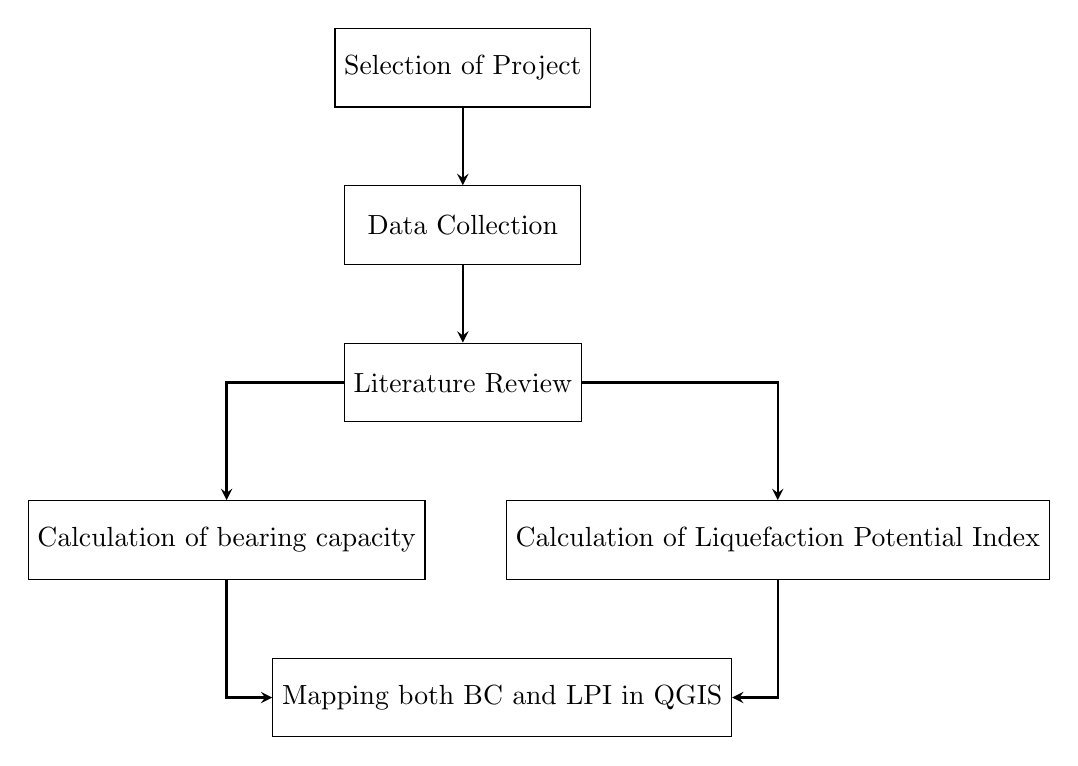
\begin{tikzpicture}[node distance=2cm]
  \node (step1) [process, xshift=2.5cm] {Selection of Project};
  \node (step2) [process, below of = step1] {Data Collection};
  \node (step3) [process, below of = step2] {Literature Review};
  \node (step4) [process, below of = step3, xshift=-3cm] {Calculation of bearing capacity};
  \node (step5) [process, right of= step4, xshift=5cm] {Calculation of Liquefaction Potential Index};
  \node (step6) [process, below of = step4, xshift=3.5cm] {Mapping both BC and LPI in QGIS};
  %now connect
  \draw [arrow] (step1) -- (step2);
  \draw [arrow] (step2) -- (step3);
  \draw [arrow] (step3) -| (step4);
  \draw [arrow] (step3) -| (step5);
  \draw [arrow] (step4) |- (step6);
  \draw [arrow] (step5) |- (step6);
  \end{tikzpicture}
  \caption{Project Flowchart}
\end{figure}

\subsection{Selection of Project}
As a matter of interest, we choose geotechnical field for our final year project. We discussed with our supervisor and attempted to try the Bearing Capacity Zonation and Liquefaction Potential Index Mapping. This project enables any future uses to find tentative bearing capacity and LPI of Kathmandu valley.

\subsection{Data Collection}
Data required for our project was SPT value and summary sheet for different locations as SPT was commonly used for bearing capacity calculation as well as LPI analysis of any place. Our data was provided by our supervisor as well as from Multilab. We collected about 104 boreholes from about 31 locations.

\subsection{Literature Review}
Detailed information about the project was needed, for that we studied various books as well as journals related to shallow foundation bearing capacity. As well as bearing capacity calculations from shear as well as deflection methods. For liquefaction we read various papers by Seed, Idris and research on Nepal earthquake 2015, etc.

\begin{wrapfigure}{r}{0.25\textwidth}
\centering
\includegraphics[width=\linewidth,keepaspectratio]{images/main/footing.png}
\caption{Footing Dimension}
\label{fsec}
\end{wrapfigure}
\subsection{Foundation Selection}
In this project work, square footing has been used. Buildings in Kathmandu valley have a depth of nearly 2m. Thus bearing capacity has been calculated for depths 1.5m, 3m and 4.5m for a footing dimension 2m * 2m as in Figure ~\ref{fsec}. Ground water table has been used as given in the bore logs. Also, the permissible settlement of 25mm is taken for settlement criteria approach.

\subsection{Calculation of bearing capacity from theoretical approaches}
The various parameters of soil like cohesion, internal angle of friction, young’s modulus of elasticity, unit weight, poisons ratio, etc were interpreted from SPT N value through various literatures available. Methods like Terzaghi, Meyerhof, Hansen, Vesic and Teng are used for the calculation of bearing capacity under shear criteria. And, Bowels, Teng, Peck and Meyerhof methods were used for settlement criteria.

\subsection{Use PLAXIS 2D for Numerical Modeling}
In this project a numerical model is developed using PLAXIS. Finite element analysis is carried out using Mohr coulomb failure criteria to represent two-dimensional soil models. Foundation is modelled as square footing and load increment is applied till the soil model fails. Ultimate bearing capacity is identified as that minimum pressure on footing at which the foundation soil experiences shear failure. And for deflection criteria, reaction at 25mm deflection is noted which is ultimate bearing capacity. In plaxis effective stress is considered as an ultimate bearing capacity.

\subsection{Calculation of liquefaction potential index}
For calculating liquefaction index, stress based approach was used and factor of safety was calculated using ratio of cyclic resistance ratio to cyclic stress ratio and from that LPI was calculated using data for up to 20m or for up to given data.

\subsection{Mapping of BC and LPI using QGIS}
We used QGIS for mapping. Map of Nepal was taken and we put our location on map. After using map of only two districts i.e. Kathmandu and Lalitpur (as our data lies on those districts). The value of all points are interpolated and clipped by our district maps. Suitable colour and map elements are selected accordingly.

IDW interpolation method was used in this software. The least value of the location was plotted. Consequently, the study area was categorized into following zones:

For Bearing Capacity:
\begin{enumerate}
\item{Weak soil region having BC $\le$ 100 kPa}
\item{Soft soil region having BC \textgreater 100 and $\le$ 150 kPa}
\item{Moderate soil region having BC \textgreater 150 and $\le$ 200 kPa}
\item{Moderately hard soil region having BC \textgreater 200 and $\le$ 250 kPa}
\item{Hard soil region having BC \textgreater 250 kPa}
\end{enumerate}

For LPI:
\begin{enumerate}
\item{Very low from 0 – 2}
\item{Low from 2 – 5}
\item{High from 5 – 15}
\item{Very high from \textgreater 15}
\end{enumerate}

\section{Determination soil properties for calculation}
\subsection{Determination of E}
The value of E can be estimated for different types of soil as given in \cite{kulhawy_manual_1990}.
\par
For cohesive soil:
\begin{equation}
\frac{E}{P_a}(kN/m^3)= \begin{cases}
    15-40 * N_{60}, & \text{for very soft soil}\\
    40-80 * N_{60}, & \text{for soft soil}\\
    80-200 * N_{60}, & \text{for compact and dense}
    \end{cases}\\
\end{equation}
\par
And for cohesionless soil:
\begin{equation}
\frac{E}{P_a}(kN/m^3)= \begin{cases}
    5 * N_{60}, & \text{with fines}\\
    10 * N_{60}, & \text{without fines}
    \end{cases}\\
\end{equation}

\subsection{Determination of C}
The values of C is determined by using Equation ~\ref{cu-form}. For cohesionless soil this value is taken as 0.

\subsection{Determination of $\phi$}
The value of $\phi$ is determined by using Equation ~\ref{phi-form}. For cohesive soil this value is taken as 0.

\subsection{Determination of $\nu$}
The value of $\nu$ is taken as:-
\begin{equation}
\nu= \begin{cases}
    0.3, & \text{for cohesionless soil}\\
    0.45, & \text{for cohesive soil}
    \end{cases}\\
\end{equation}

\subsection{Determination of other parameters}
Other parameters are calculated from Emperical Formulas in subsection ~\ref{emp-form}.

\section{Removing Outliers}
The outliers were removed by calculating $Q_1$ and $Q_3$ and calculating $IQD$. Then only values that were between $Q_1 - 1.5$ ILD and $Q_3 + 1.5$ ILD were selected for further calculation like mean and standard deviation.

\section{Selection Median}
In summary Terzaghi was excluded from shear since it has no depth corrections. Meyerhof ,Hansen, and Vesic give similar results so their average was used as a value. Finally median for summary was selected from every such values in that locations.

\section{Correlation and Regression}
Pearson’s Correlation was used for correlation. The regression was obtained by fitting 1st degree polynomial. The value of Pearson’s Correlation lies between -1 to +1. where
\begin{itemize}
\item \textbf{Positive Correlation}: both variables change in the same direction.
\item \textbf{Neutral Correlation}: No relationship in the change of the variables.
\item \textbf{Negative Correlation}: variables change in opposite directions.
\end{itemize}
	%now Results
	\chapter{Result}
104 Borehole Log Data of 31 locations inside Kathmandu and Lalitpur district areas were taken into consideration. The results were obtained after calculating Bearing Capacity at 1.5m, 3m, and 4.5m depth by shear criteria using Terzaghi, Meyerhof, Hansen, Vesic and Teng methods and Plaxis2D software and by deflection criteria using Bowels, Teng, Peck, Meyerhof  methods and Plaxis2D software. The median value of those methods are taken and mapped for those depths. Liquifaction Potential Index of the area is also mapped.
\pagebreak

\section{Location Table}
\begin{table}[!h]
\caption{Location Table}
\begin{tabularx}{\textwidth}{ | l | p{0.6\textwidth} | X | X | }
\hline
 \textbf{S.N.} & \textbf{Location} & \textbf{Latitude} & \textbf{Longitude} \\
\hline
 1 & Rastriya Banijya Bank: Thapathali, Kathmandu & 27.65586 & 85.30645 \\
 2 & Building Complex: Anamnagar, Kathmandu & 27.69728 & 85.32746 \\
 3 & Building Complex: Bakhundol Lalitpur & 27.68302 & 85.31033 \\
 4 & Hindu vidhypeth: Balkumari, Lalitpur & 27.67114 & 85.33793 \\
 5 & DI Skin Health and Referral Center (P). Ltd.: Bansbari, Kathmandu & 27.73704 & 85.33354 \\
 6 & Building: Bhaisipati, Lalitpur & 27.64805 & 85.29596 \\
 7 & Brihaspati Vidyasadan School: Gahanapokhari, Kathmandu & 27.71425 & 85.32957 \\
 8 & Green Hill City (P). Ltd. : Mulpani, Kathamndu  & 27.71577 & 85.38647 \\
 9 & Building Site: Itachhe tol, Bhaktapur & 27.67284 & 85.42261 \\
 10 & Buddha Air (P). Ltd. : Jawalakhel, Lalitpur  & 27.67357 & 85.31187 \\
 11 & Tamrakar Samaj: Jawalakhel & 27.67475 & 85.31220 \\
 12 & Tangal, Kathmandu & 27.72009 & 85.32626 \\
 13 & Harihar Bhavan, Lalitpur & 27.68047 & 85.31111 \\
 14 & Janamaitri Campus: Kuleswore, Kathmandu & 27.69173 & 85.29005 \\
 15 & Amrit Science Campus: Lainchour, Kathmandu & 27.71776 & 85.31061 \\
 16 & Mahendra Ratna Campus: Tahachal, Kathmandu & 27.70346 & 85.29821 \\
 17 & Bhatbhateni Supermarket \& Departmental Store: Satdobato, Lalitpur & 27.65712 & 85.32002 \\
 18 & Nepal Mountaineering Association :  Naxal, Nagpokhari Kathmandu  & 27.71303 & 85.32167 \\
 19 & Patanjali Yogpeeth Nepal : Mandikatar, Kathmandu  & 27.74115 & 85.34555 \\
 20 & Mandikhatar, Kathmandu  & 27.73878 & 85.34535 \\
 21 & CIWEC Clinic: Lainchaur, Kathmandu  & 27.72040 & 85.31555 \\
 22 & Vastukala Pharamarsha Nepal : Kupondole, Lalitpur & 27.68376 & 85.31634 \\
 23 & Building: Kupondole, Lalitpur & 27.68628 & 85.31470 \\
 24 & NAST Technology : Khumaltar, Lalitpur & 27.65610 & 85.32768 \\
 25 & Building: Khumaltar, Lalitpur  & 27.64870 & 85.32034 \\
 26 & Building: Kalopul, Pumori, Kathmandu & 27.71183 & 85.33536 \\
 27 & Building Site : Gwarkho, Lalitpur & 27.66601 & 85.32847 \\
 28 & Building: Kumaripati, Lalitpur & 27.67025 & 85.31863 \\
 29 & Building: Kupandole, Lalitpur & 27.68703 & 85.30930 \\
 30 & Nepal Rastra Bank: Thapathali & 27.69023 & 85.31993 \\
 31 & Exam Mega Hall Construction Project : Kirtipur, Kathmandu & 27.68426 & 85.29536 \\
\hline
\end{tabularx}

\end{table}
\pagebreak

\section{Locations map\index{map}}
\begin{figure}[!hbt]
\centering
\includegraphics[width=\linewidth, height=\textheight,keepaspectratio]{in/map/Borehole2.png}
\caption{Borehole locations\index{map}}
\end{figure}
\pagebreak

\section{Shear Strength Table(KPa)}
\begin{table}[!h]
\caption{Shear Strength Table}
\begin{tabularx}{\textwidth}{ | l | p{0.5\textwidth} | X | X | X | }
\hline
 \textbf{S.N.} & \textbf{Location} & \textbf{1.5m} & \textbf{3.0m} & \textbf{4.5m}\\
\hline
 1 & Thapathali, Kathmandu & 556.783 & 881.966 & 1219.911 \\
 2 & Anamnagar, Kathmandu & 226.203 & 253.102 & 210.010 \\
 3 & Bakhundol Lalitpur & 78.274 & 109.557 & 126.082 \\
 4 & Balkumari, Lalitpur & 347.149 & 705.395 & 497.897 \\
 5 & Bansbari, Kathmandu & 226.203 & 411.124 & 573.964 \\
 6 & Bhaisipati, Lalitpur & 318.034 & 654.486 & 375.495 \\
 7 & Gahanapokhari, Kathmandu & 160.596 & 211.665 & 408.875 \\
 8 & Mulpani, Kathamndu  & 85.764 & 155.830 & 738.492 \\
 9 & Itachhe tol, Bhaktapur & 103.915 & 141.288 & 161.811 \\
 10 & Jawalakhel, Lalitpur  & 295.379 & 525.479 & 351.012 \\
 11 & Jawalakhel & 154.538 & 188.042 & 218.952 \\
 12 & Tangal, Kathmandu & 818.280 & 1500.181 & 1701.000 \\
 13 & Harihar Bhavan, Lalitpur & 678.380 & 862.325 & 1080.162 \\
 14 & Kuleswore, Kathmandu & 258.687 & 440.825 & 510.316 \\
 15 & Lainchour, Kathmandu & 427.627 & 1031.251 & 1534.093 \\
 16 & Tahachal, Kathmandu & 213.742 & 278.658 & 324.310 \\
 17 & Satdobato, Lalitpur & 664.956 & 750.835 & 216.900 \\
 18 & Naxal, Nagpokhari Kathmandu  & 661.987 & 1034.337 & 1088.942 \\
 19 & Mandikatar, Kathmandu  & 216.255 & 558.979 & 750.723 \\
 20 & Mandikhatar, Kathmandu  & 166.394 & 374.942 & 819.365 \\
 21 & Lainchaur, Kathmandu  & 961.112 & 1349.100 & 1269.905 \\
 22 & Kupondole, Lalitpur & 197.198 & 707.709 & 1129.132 \\
 23 & Kupondole, Lalitpur & 177.101 & 213.827 & 248.214 \\
 24 & Khumaltar, Lalitpur & 130.857 & 158.837 & 179.932 \\
 25 & Khumaltar, Lalitpur  & 113.986 & 140.911 & 169.485 \\
 26 & Kalopul, Pumori, Kathmandu & 702.484 & 1078.437 & 1160.662 \\
 27 & Gwarkho, Lalitpur & 101.891 & 139.931 & 175.822 \\
 28 & Kumaripati, Lalitpur & 976.011 & 1705.445 & 1978.329 \\
 29 & Kupandole, Lalitpur & 107.883 & 127.698 & 152.281 \\
 30 & Thapathali & 381.822 & 577.350 & 761.849 \\
 31 & Kirtipur, Kathmandu & 363.008 & 713.392 & 1008.880 \\
\hline
\multicolumn{2}{|X|}{\mbox{Mean($\overline{x}$)}} & 350.726 & 580.094 & 682.026 \\
\multicolumn{2}{|X|}{\mbox{Standard deviation($\sigma$)}} & 262.236 & 428.627 & 505.678 \\
\multicolumn{2}{|X|}{\mbox{Minimum($x_{min}$)}} & 78.274 & 109.557 & 126.082 \\
\multicolumn{2}{|X|}{\mbox{Maximum($x_{max}$)}} & 976.011 & 1705.445 & 1978.329 \\
\hline
\end{tabularx}

\end{table}
\pagebreak

\section{1.5m Bearing Capacity(shear)\index{map}}
\begin{figure}[!hbt]
\centering
\includegraphics[width=\linewidth, height=\textheight,keepaspectratio]{in/map/Shear_1_5.png}
\caption{BC at 1.5m depth}
\end{figure}
\pagebreak

\section{3.0m Bearing Capacity(shear)\index{map}}
\begin{figure}[!hbt]
\centering
\includegraphics[width=\linewidth, height=\textheight,keepaspectratio]{in/map/Shear_3_0.png}
\caption{BC at 3.0m depth}
\end{figure}
\pagebreak

\section{4.5m Bearing Capacity(shear)\index{map}}
\begin{figure}[!hbt]
\centering
\includegraphics[width=\linewidth, height=\textheight,keepaspectratio]{in/map/Shear_4_5.png}
\caption{BC at 4.5m depth}
\end{figure}
\pagebreak

\section{Settlement Strength Table(KPa, for 25mm)}
\begin{table}[!h]
\caption{Settlement Strength Table}
\input{../proj/soilbearing/secrets/settlement_table}
\end{table}
\pagebreak

\section{1.5m Bearing Capacity(settlement)\index{map}}
\begin{figure}[!hbt]
\centering
\includegraphics[width=\linewidth, height=\textheight,keepaspectratio]{in/map/Deflection_1_5.png}
\caption{BC at 1.5m depth}
\end{figure}
\pagebreak

\section{3.0m Bearing Capacity(settlement)\index{map}}
\begin{figure}[!hbt]
\centering
\includegraphics[width=\linewidth, height=\textheight,keepaspectratio]{in/map/Deflection_3_0.png}
\caption{BC at 3.0m depth}
\end{figure}
\pagebreak

\section{4.5m Bearing Capacity(settlement)\index{map}}
\begin{figure}[!hbt]
\centering
\includegraphics[width=\linewidth, height=\textheight,keepaspectratio]{in/map/Deflection_4_5.png}
\caption{BC at 4.5m depth}
\end{figure}
\pagebreak

\section{Liquefaction(LPI) Table}
\begin{table}[!h]
\caption{Liquefaction(LPI) Table}
\begin{tabularx}{\textwidth}{ | l | p{0.5\textwidth} | X | }
\hline
 \textbf{S.N.} & \textbf{Location} & \textbf{LPI}\\
\hline
 1 & Thapathali, Kathmandu & 26.184 \\
 2 & Anamnagar, Kathmandu & 18.597 \\
 3 & Bakhundol Lalitpur & 6.858 \\
 4 & Balkumari, Lalitpur & 16.423 \\
 5 & Bansbari, Kathmandu & 1.518 \\
 6 & Bhaisipati, Lalitpur & 0.045 \\
 7 & Gahanapokhari, Kathmandu & 0.670 \\
 8 & Mulpani, Kathamndu  & 1.325 \\
 9 & Itachhe tol, Bhaktapur & 0.479 \\
 10 & Jawalakhel, Lalitpur  & 0.743 \\
 11 & Jawalakhel & 12.442 \\
 12 & Tangal, Kathmandu & 4.132 \\
 13 & Harihar Bhavan, Lalitpur & 31.190 \\
 14 & Kuleswore, Kathmandu & 17.653 \\
 15 & Lainchour, Kathmandu & 1.319 \\
 16 & Tahachal, Kathmandu & 50.302 \\
 17 & Satdobato, Lalitpur & 0.383 \\
 18 & Naxal, Nagpokhari Kathmandu  & 1.661 \\
 19 & Mandikatar, Kathmandu  & 1.028 \\
 20 & Mandikhatar, Kathmandu  & 2.204 \\
 21 & Lainchaur, Kathmandu  & 4.616 \\
 22 & Kupondole, Lalitpur & 2.649 \\
 23 & Kupondole, Lalitpur & 10.705 \\
 24 & Khumaltar, Lalitpur & 16.796 \\
 25 & Khumaltar, Lalitpur  & 11.200 \\
 26 & Kalopul, Pumori, Kathmandu & 6.137 \\
 27 & Gwarkho, Lalitpur & 19.032 \\
 28 & Kumaripati, Lalitpur & 0.000 \\
 29 & Kupandole, Lalitpur & 20.590 \\
 30 & Thapathali & 4.920 \\
 31 & Kirtipur, Kathmandu & 8.512 \\
\hline
\multicolumn{2}{|X|}{\mbox{Mean($\overline{x}$)}} & 8.334  \\
\multicolumn{2}{|X|}{\mbox{Standard deviation($\sigma$)}} & 8.579 \\
\multicolumn{2}{|X|}{\mbox{Minimum($x_{min}$)}} & 0.000 \\
\multicolumn{2}{|X|}{\mbox{Maximum($x_{max}$)}} & 31.190 \\
\hline
\end{tabularx}

\end{table}
\pagebreak

\section{LPI\index{map}}
\begin{figure}[!hbt]
\centering
\includegraphics[width=\linewidth, height=\textheight,keepaspectratio]{in/map/lqi2.png}
\caption{LPI}
\end{figure}
\pagebreak
	\chapter{Discussion}
Calculation of bearing capacity of soil has significant importance especially in urban areas like Kathmandu Valley where maximum land area is being used on building construction and the inadequacy of remaining land means high rise buildings are being constructed more and more. We can interpret the maps shown above to figure out the soil’s bearing capacity and liquefaction potential which determines the feasibility of construction in that area. 

The value of bearing capacity and LPI can be interpreted as shown below

\begin{itemize}
\item Region having bearing capacity $\le$ 100Kpa 			: Weak soil
\item Region having bearing capacity \textgreater 100Kpa and $\le$150Kpa	: Soft soil
\item Region having bearing capacity \textgreater 150Kpa and $\le$200Kpa	: Medium soil
\item Region having bearing capacity \textgreater 200Kpa and $\le$250Kpa	: Moderately hard soil
\item Region having bearing capacity \textgreater 250Kpa			: Hard soil
\end{itemize}

For LPI value of soil:
\begin{itemize}
\item LPI 0-2: Very low potential
\item LPI 2-5: Low potential
\item LPI 5-15: High potential
\item LPI >15: Very High potential
\end{itemize}

\section{Summary of bearing capacity at diffrent depths}
\subsection{Bearing Capacity at 1.5m depth}
At 1.5m depth, by shear failure criteria, the highest bearing capacity was found as 1135.052KPa at Kumaripati and the lowest bearing capacity was found at Bakhundol which was 75.880KPa. By deflection criteria, the highest value was at Satdobato as 216.65KPa and lowest value was 24.68 at Bakhundol.
For shear criteria, the soil at Bakhundol, Mulpani, Itachhe Tol, Jawalakhel, Khumaltar, Gwarko and Kupondole were found to be weak soils as their Bearing capacity value was less than 100KPa. The soil at Thapathali, Tangal, Harihar Bhavan, Lainchaur, Pumori and Kumaripati were found to be hard soil with bearing capacity greater than 250KPa.

\subsection{Bearing Capacity at 3m depth}
At 1.5m depth, by shear failure criteria, the highest bearing capacity was found as 1115.63KPa at Kumaripati and the lowest bearing capacity was found at Bakhundol which was 52.49KPa. By deflection criteria, the highest value was at Bhaisipati as 197.93KPa and lowest value was 31.88KPa at Bakhundol.
By shear failure criteria, Bakhundol, Mulpani, Itachhe Tol, Jawalakhel, Khumaltar, Gwarko and Kupondole were found to be weak soils as their Bearing capacity value was less than 100KPa. The soil at Thapathali, Balkumari, Bansbari, Tangal, Harihar Bhavan, Lainchour, Satdobato, Nagpokhari, Lainchaur, Kupondole, Pumori, Kumaripati, Thapathali were found to be hard soils with bearing capacity greater than 250KPa.

\subsection{Bearing Capacity at 4.5m depth}
At 4.5m depth, by shear failure criteria, the highest bearing capacity was found as 1700.13KPa at Kumaripati and the lowest bearing capacity was found at Bakhundol which was 54.51KPa. By deflection criteria, the highest value was at Bhaisipati as 181.51KPa and lowest value was 37.26KPa at Bakhundol.
By shear failure criteria, Anamnagar, Bakhundol, Itachhe Tol, Jawalakhel, Khumaltar, Gwarko and Kupondole were found to have weak soils as their Bearing capacity value was less than 100KPa. The soil at Thapathali, Balkumari, Mulpani, Tangal, Harihar Bhavan, Kuleswore, Lainchour, Nagpokhari, Mandikatar, Lainchaur, Kupondole, Pumori, Kumaripati, Thapathali and Kirtipur were found to be hard soils with bearing capacity greater than 250KPa.

\subsection{Liquefaction Potential}
The LPI value was found to be the highest at Tahachal with a calue of 50.30 and was the lowest at Kumaripati with a value of 0.00.
Bansbari, Bhaisepati, Gahanapokhari, Mulpani, Itachhe Tol, Jawalakhel, Satdobato, Nagpokhari, Mandikar and Kumaripati had very low liquefaction potential as their LPI value was found to be less than 2. Places like Thapathali, Anamnagar, Balkumari, Harihar Bhavan, Kuleswore,Tahachal, Khumaltar, Gwarko and kupandole had very high potential for liquefaction as their LPI value was greater than 15.
	\chapter{Conclusion}
Using the 104 Borehole logs from 31 different locations throughout Kathmandu valley, mapping and zonation of bearing capacity and Liquefaction Potential Index were carried out. By analysis of those maps, following conclusions can be reached:

\begin{itemize}
\item The maps produced are powerful tools for the visualization of soil properties which can save time and cost to figure out the preliminary information of the soil required and the bearing capacity and LPI value to be expected.
\item The maps can serve as a guidance tools for engineers to figure out the suitability of any type of construction in the area, the need of treatments, type of foundation etc.
\item The bearing capacity of the soil depends upon the method used.
\item The LPI index map can be used as a hazard map on where liquefaction can be expected and where treatments need to be done.
\item Liquefaction potential was found to be strongly influenced by SPT value and the depth of water table.
\item The soil deposit of Kathmandu valley was found to be highly heterogeneous with extensively varying soil content and water table depth which means the bearing capacity and LPI value of the soil can change even in small distances.
\end{itemize}

	%Followed by annex
	\appendix
		\chapter{Table and Calculations}
\blfootnote{* Means the datas are shown only but not used for further calculation}
{\large \textbf{Rastriya Banijya Bank: Thapathali, Kathmandu}}\newline
\begin{tabularx}{\textwidth}{ | p{0.15cm} | X | X | X | p{1.3cm} | p{1.3cm} | X | p{1.3cm} |}
\hline
\multicolumn{4}{|X|}{\textbf{Borehole:}1} & \multicolumn{4}{X|}{\textbf{LPI}:21.18} \\
\hline
\multirow{4}{*}{\rotatebox[origin=c]{90}{\textbf{Shear}}} & \textbf{Depth} & \textbf{Terzaghi}* & \textbf{Meyerhof} & \textbf{Hansen} & \textbf{Vesic} & \textbf{Plaxis} & \textbf{Teng} \\
\cline{2-8}
  & \textbf{1.5} & 400.72 & 513.58 & 558.16 & 575.03 & 797.05 & 61.02 \\
  & \textbf{3.0} & 541.92 & 783.32 & 900.40 & 917.27 & 1135.85 & 104.28 \\
  & \textbf{4.5} & 657.36 & 1057.54 & 1268.90 & 1285.77 & 1455.67 & 167.25 \\
\hline
\multirow{4}{*}{\rotatebox[origin=c]{90}{\textbf{Settlement}}} & \textbf{Depth} & \textbf{Bowels} & \textbf{Plaxis} & \textbf{Peck} & \textbf{Teng} & \textbf{Meyerhof} & \textbf{WL} \\
\cline{2-8}
 & \textbf{1.5} & 43.73 & 40.06 & 31.95 & 13.80 & 29.15 & \multirow{3}{*}{1.50 m} \\
  & \textbf{3.0} & 63.42 & 51.64 & 39.54 & 33.96 & 42.28 & \\
  & \textbf{4.5} & 84.17 & 61.72 & 49.69 & 56.44 & 56.11 & \\
 \hline
\end{tabularx}
\newline\break
\begin{tabularx}{\textwidth}{ | p{0.15cm} | X | X | X | p{1.3cm} | p{1.3cm} | X | p{1.3cm} |}
\hline
\multicolumn{4}{|X|}{\textbf{Borehole:}2} & \multicolumn{4}{X|}{\textbf{LPI}:28.43} \\
\hline
\multirow{4}{*}{\rotatebox[origin=c]{90}{\textbf{Shear}}} & \textbf{Depth} & \textbf{Terzaghi}* & \textbf{Meyerhof} & \textbf{Hansen} & \textbf{Vesic} & \textbf{Plaxis} & \textbf{Teng} \\
\cline{2-8}
  & \textbf{1.5} & 361.88 & 458.67 & 504.16 & 518.97 & 713.32 & 61.02 \\
  & \textbf{3.0} & 486.48 & 696.16 & 807.08 & 821.89 & 1023.04 & 94.75 \\
  & \textbf{4.5} & 586.90 & 935.09 & 1131.52 & 1146.34 & 1366.96 & 133.58 \\
\hline
\multirow{4}{*}{\rotatebox[origin=c]{90}{\textbf{Settlement}}} & \textbf{Depth} & \textbf{Bowels} & \textbf{Plaxis} & \textbf{Peck} & \textbf{Teng} & \textbf{Meyerhof} & \textbf{WL} \\
\cline{2-8}
 & \textbf{1.5} & 43.73 & 36.16 & 31.95 & 13.80 & 29.15 & \multirow{3}{*}{1.50 m} \\
  & \textbf{3.0} & 52.40 & 44.30 & 32.67 & 22.03 & 34.93 & \\
  & \textbf{4.5} & 59.92 & 52.20 & 35.37 & 30.17 & 39.94 & \\
 \hline
\end{tabularx}
\newline\break
\begin{tabularx}{\textwidth}{ | p{0.15cm} | X | X | X | p{1.3cm} | p{1.3cm} | X | p{1.3cm} |}
\hline
\multicolumn{4}{|X|}{\textbf{Borehole:}3} & \multicolumn{4}{X|}{\textbf{LPI}:28.18} \\
\hline
\multirow{4}{*}{\rotatebox[origin=c]{90}{\textbf{Shear}}} & \textbf{Depth} & \textbf{Terzaghi}* & \textbf{Meyerhof} & \textbf{Hansen} & \textbf{Vesic} & \textbf{Plaxis} & \textbf{Teng} \\
\cline{2-8}
  & \textbf{1.5} & 413.17 & 530.26 & 572.99 & 590.67 & 815.45 & 61.12 \\
  & \textbf{3.0} & 563.74 & 815.20 & 937.30 & 954.14 & 1148.95 & 99.64 \\
  & \textbf{4.5} & 678.57 & 1092.96 & 1307.95 & 1324.79 & 1530.37 & 138.60 \\
\hline
\multirow{4}{*}{\rotatebox[origin=c]{90}{\textbf{Settlement}}} & \textbf{Depth} & \textbf{Bowels} & \textbf{Plaxis} & \textbf{Peck} & \textbf{Teng} & \textbf{Meyerhof} & \textbf{WL} \\
\cline{2-8}
 & \textbf{1.5} & 45.92 & 37.97 & 32.58 & 14.49 & 30.61 & \multirow{3}{*}{1.60 m} \\
  & \textbf{3.0} & 55.85 & 47.59 & 35.36 & 25.77 & 37.23 & \\
  & \textbf{4.5} & 62.30 & 53.22 & 37.24 & 32.75 & 41.53 & \\
 \hline
\end{tabularx}
\newline\break
\begin{tabularx}{\textwidth}{ | p{0.15cm} | X | X | X | p{1.3cm} | p{1.3cm} | X | p{1.3cm} |}
\hline
\multicolumn{4}{|X|}{\textbf{Borehole:}4} & \multicolumn{4}{X|}{\textbf{LPI}:26.95} \\
\hline
\multirow{4}{*}{\rotatebox[origin=c]{90}{\textbf{Shear}}} & \textbf{Depth} & \textbf{Terzaghi}* & \textbf{Meyerhof} & \textbf{Hansen} & \textbf{Vesic} & \textbf{Plaxis} & \textbf{Teng} \\
\cline{2-8}
  & \textbf{1.5} & 417.12 & 535.87 & 575.57 & 594.13 & 801.37 & 61.23 \\
  & \textbf{3.0} & 560.92 & 811.16 & 931.39 & 948.26 & 1106.70 & 102.41 \\
  & \textbf{4.5} & 675.75 & 1088.39 & 1301.00 & 1317.87 & 1395.57 & 149.28 \\
\hline
\multirow{4}{*}{\rotatebox[origin=c]{90}{\textbf{Settlement}}} & \textbf{Depth} & \textbf{Bowels} & \textbf{Plaxis} & \textbf{Peck} & \textbf{Teng} & \textbf{Meyerhof} & \textbf{WL} \\
\cline{2-8}
 & \textbf{1.5} & 48.11 & 38.56 & 33.22 & 15.18 & 32.07 & \multirow{3}{*}{1.70 m} \\
  & \textbf{3.0} & 56.61 & 48.77 & 36.39 & 26.60 & 37.74 & \\
  & \textbf{4.5} & 68.80 & 56.21 & 41.63 & 39.80 & 45.87 & \\
 \hline
\end{tabularx}
\newline\break
\textbf{Summary:}\newline
\begin{tabularx}{\textwidth}{ | X | X | X | X | X | X | }
\hline
 \textbf{Depth} & \textbf{Shear} & \textbf{Deflection} & \textbf{LPI} & \textbf{Latitude} & \textbf{Longitude}\\
\hline
 \textbf{1.5} & 556.78 & 32.33 & \multirow{3}{*}{26.18} & \multirow{3}{*}{27.655862} & \multirow{3}{*}{85.306446} \\
 \textbf{3.0} & 881.97 & 38.64 & & & \\
 \textbf{4.5} & 1219.91 & 50.94 & & & \\
\hline
\end{tabularx}
\hfill\break
\newline
{\large \textbf{Building Complex: Anamnagar, Kathmandu}}\newline
\begin{tabularx}{\textwidth}{ | p{0.15cm} | X | X | X | p{1.3cm} | p{1.3cm} | X | p{1.3cm} |}
\hline
\multicolumn{4}{|X|}{\textbf{Borehole:}1} & \multicolumn{4}{X|}{\textbf{LPI}:17.96} \\
\hline
\multirow{4}{*}{\rotatebox[origin=c]{90}{\textbf{Shear}}} & \textbf{Depth} & \textbf{Terzaghi}* & \textbf{Meyerhof} & \textbf{Hansen} & \textbf{Vesic} & \textbf{Plaxis} & \textbf{Teng} \\
\cline{2-8}
  & \textbf{1.5} & 90.35 & 86.33 & 104.61 & 104.61 & 215.36 & 209.84 \\
  & \textbf{3.0} & 438.05 & 608.77 & 763.50 & 776.78 & 111.02 & 241.35 \\
  & \textbf{4.5} & 85.99 & 104.49 & 100.26 & 100.26 & 148.95 & 215.91 \\
\hline
\multirow{4}{*}{\rotatebox[origin=c]{90}{\textbf{Settlement}}} & \textbf{Depth} & \textbf{Bowels} & \textbf{Plaxis} & \textbf{Peck} & \textbf{Teng} & \textbf{Meyerhof} & \textbf{WL} \\
\cline{2-8}
 & \textbf{1.5} & 267.86 & 42.48 & 145.35 & 217.45 & 178.57 & \multirow{3}{*}{3.00 m} \\
  & \textbf{3.0} & 121.56 & 50.47 & 93.28 & 96.92 & 81.04 & \\
  & \textbf{4.5} & 88.37 & 57.19 & 61.94 & 60.98 & 58.91 & \\
 \hline
\end{tabularx}
\newline\break
\begin{tabularx}{\textwidth}{ | p{0.15cm} | X | X | X | p{1.3cm} | p{1.3cm} | X | p{1.3cm} |}
\hline
\multicolumn{4}{|X|}{\textbf{Borehole:}2} & \multicolumn{4}{X|}{\textbf{LPI}:18.83} \\
\hline
\multirow{4}{*}{\rotatebox[origin=c]{90}{\textbf{Shear}}} & \textbf{Depth} & \textbf{Terzaghi}* & \textbf{Meyerhof} & \textbf{Hansen} & \textbf{Vesic} & \textbf{Plaxis} & \textbf{Teng} \\
\cline{2-8}
  & \textbf{1.5} & 341.14 & 441.45 & 427.08 & 455.73 & 105.38 & 212.41 \\
  & \textbf{3.0} & 110.15 & 118.98 & 127.54 & 127.54 & 150.25 & 226.62 \\
  & \textbf{4.5} & 106.34 & 128.89 & 123.73 & 123.73 & 176.62 & 209.63 \\
\hline
\multirow{4}{*}{\rotatebox[origin=c]{90}{\textbf{Settlement}}} & \textbf{Depth} & \textbf{Bowels} & \textbf{Plaxis} & \textbf{Peck} & \textbf{Teng} & \textbf{Meyerhof} & \textbf{WL} \\
\cline{2-8}
 & \textbf{1.5} & 283.17 & 59.81 & 149.83 & 229.87 & 188.78 & \multirow{3}{*}{3.20 m} \\
  & \textbf{3.0} & 125.98 & 61.37 & 90.08 & 98.24 & 83.99 & \\
  & \textbf{4.5} & 82.64 & 64.32 & 59.15 & 54.78 & 55.09 & \\
 \hline
\end{tabularx}
\newline\break
\begin{tabularx}{\textwidth}{ | p{0.15cm} | X | X | X | p{1.3cm} | p{1.3cm} | X | p{1.3cm} |}
\hline
\multicolumn{4}{|X|}{\textbf{Borehole:}3} & \multicolumn{4}{X|}{\textbf{LPI}:19.06} \\
\hline
\multirow{4}{*}{\rotatebox[origin=c]{90}{\textbf{Shear}}} & \textbf{Depth} & \textbf{Terzaghi}* & \textbf{Meyerhof} & \textbf{Hansen} & \textbf{Vesic} & \textbf{Plaxis} & \textbf{Teng} \\
\cline{2-8}
  & \textbf{1.5} & 320.32 & 411.62 & 416.47 & 439.77 & 110.51 & 203.43 \\
  & \textbf{3.0} & 114.87 & 124.19 & 133.23 & 133.23 & 156.63 & 253.10 \\
  & \textbf{4.5} & 110.42 & 134.24 & 128.78 & 128.78 & 184.16 & 243.34 \\
\hline
\multirow{4}{*}{\rotatebox[origin=c]{90}{\textbf{Settlement}}} & \textbf{Depth} & \textbf{Bowels} & \textbf{Plaxis} & \textbf{Peck} & \textbf{Teng} & \textbf{Meyerhof} & \textbf{WL} \\
\cline{2-8}
 & \textbf{1.5} & 229.59 & 58.46 & 134.17 & 186.38 & 153.06 & \multirow{3}{*}{2.50 m} \\
  & \textbf{3.0} & 134.98 & 70.76 & 97.11 & 111.46 & 89.98 & \\
  & \textbf{4.5} & 107.42 & 68.43 & 71.34 & 81.61 & 71.61 & \\
 \hline
\end{tabularx}
\newline\break
\begin{tabularx}{\textwidth}{ | p{0.15cm} | X | X | X | p{1.3cm} | p{1.3cm} | X | p{1.3cm} |}
\hline
\multicolumn{4}{|X|}{\textbf{Borehole:}4} & \multicolumn{4}{X|}{\textbf{LPI}:17.17} \\
\hline
\multirow{4}{*}{\rotatebox[origin=c]{90}{\textbf{Shear}}} & \textbf{Depth} & \textbf{Terzaghi}* & \textbf{Meyerhof} & \textbf{Hansen} & \textbf{Vesic} & \textbf{Plaxis} & \textbf{Teng} \\
\cline{2-8}
  & \textbf{1.5} & 333.22 & 429.85 & 432.88 & 457.05 & 544.20 & 226.20 \\
  & \textbf{3.0} & 499.56 & 699.67 & 868.35 & 883.39 & 488.90 & 326.95 \\
  & \textbf{4.5} & 642.22 & 996.81 & 1309.97 & 1325.25 & 244.34 & 285.55 \\
\hline
\multirow{4}{*}{\rotatebox[origin=c]{90}{\textbf{Settlement}}} & \textbf{Depth} & \textbf{Bowels} & \textbf{Plaxis} & \textbf{Peck} & \textbf{Teng} & \textbf{Meyerhof} & \textbf{WL} \\
\cline{2-8}
 & \textbf{1.5} & 245.99 & 35.11 & 143.76 & 202.95 & 164.00 & \multirow{3}{*}{2.50 m} \\
  & \textbf{3.0} & 162.80 & 40.92 & 117.13 & 141.59 & 108.54 & \\
  & \textbf{4.5} & 123.89 & 48.16 & 82.28 & 99.45 & 82.59 & \\
 \hline
\end{tabularx}
\newline\break
\begin{tabularx}{\textwidth}{ | p{0.15cm} | X | X | X | p{1.3cm} | p{1.3cm} | X | p{1.3cm} |}
\hline
\multicolumn{4}{|X|}{\textbf{Borehole:}5} & \multicolumn{4}{X|}{\textbf{LPI}:19.98} \\
\hline
\multirow{4}{*}{\rotatebox[origin=c]{90}{\textbf{Shear}}} & \textbf{Depth} & \textbf{Terzaghi}* & \textbf{Meyerhof} & \textbf{Hansen} & \textbf{Vesic} & \textbf{Plaxis} & \textbf{Teng} \\
\cline{2-8}
  & \textbf{1.5} & 359.37 & 468.32 & 467.10 & 493.09 & 447.98 & 276.46 \\
  & \textbf{3.0} & 528.90 & 741.57 & 922.27 & 937.55 & 441.02 & 356.06 \\
  & \textbf{4.5} & 670.65 & 1039.91 & 1373.56 & 1388.69 & 210.01 & 321.70 \\
\hline
\multirow{4}{*}{\rotatebox[origin=c]{90}{\textbf{Settlement}}} & \textbf{Depth} & \textbf{Bowels} & \textbf{Plaxis} & \textbf{Peck} & \textbf{Teng} & \textbf{Meyerhof} & \textbf{WL} \\
\cline{2-8}
 & \textbf{1.5} & 278.79 & 53.13 & 162.92 & 236.09 & 185.86 & \multirow{3}{*}{2.50 m} \\
  & \textbf{3.0} & 172.54 & 61.22 & 124.13 & 152.14 & 115.03 & \\
  & \textbf{4.5} & 136.43 & 64.94 & 90.60 & 113.03 & 90.95 & \\
 \hline
\end{tabularx}
\newline\break
\textbf{Summary:}\newline
\begin{tabularx}{\textwidth}{ | X | X | X | X | X | X | }
\hline
 \textbf{Depth} & \textbf{Shear} & \textbf{Deflection} & \textbf{LPI} & \textbf{Latitude} & \textbf{Longitude}\\
\hline
 \textbf{1.5} & 226.20 & 178.57 & \multirow{3}{*}{18.60} & \multirow{3}{*}{27.697282} & \multirow{3}{*}{85.327457} \\
 \textbf{3.0} & 253.10 & 98.24 & & & \\
 \textbf{4.5} & 210.01 & 71.61 & & & \\
\hline
\end{tabularx}
\hfill\break
\newline
{\large \textbf{Building Complex: Bakhundol Lalitpur}}\newline
\begin{tabularx}{\textwidth}{ | p{0.15cm} | X | X | X | p{1.3cm} | p{1.3cm} | X | p{1.3cm} |}
\hline
\multicolumn{4}{|X|}{\textbf{Borehole:}1} & \multicolumn{4}{X|}{\textbf{LPI}:7.41} \\
\hline
\multirow{4}{*}{\rotatebox[origin=c]{90}{\textbf{Shear}}} & \textbf{Depth} & \textbf{Terzaghi}* & \textbf{Meyerhof} & \textbf{Hansen} & \textbf{Vesic} & \textbf{Plaxis} & \textbf{Teng} \\
\cline{2-8}
  & \textbf{1.5} & 70.55 & 67.41 & 81.68 & 81.68 & 87.66 & 57.16 \\
  & \textbf{3.0} & 70.55 & 76.20 & 81.68 & 81.68 & 108.04 & 111.07 \\
  & \textbf{4.5} & 70.55 & 84.99 & 81.68 & 81.68 & 124.10 & 169.87 \\
\hline
\multirow{4}{*}{\rotatebox[origin=c]{90}{\textbf{Settlement}}} & \textbf{Depth} & \textbf{Bowels} & \textbf{Plaxis} & \textbf{Peck} & \textbf{Teng} & \textbf{Meyerhof} & \textbf{WL} \\
\cline{2-8}
 & \textbf{1.5} & 65.60 & 39.24 & 45.52 & 5.52 & 43.73 & \multirow{3}{*}{6.00 m} \\
  & \textbf{3.0} & 67.50 & 44.17 & 35.61 & 3.67 & 45.00 & \\
  & \textbf{4.5} & 66.75 & 48.14 & 35.18 & 11.53 & 44.50 & \\
 \hline
\end{tabularx}
\newline\break
\begin{tabularx}{\textwidth}{ | p{0.15cm} | X | X | X | p{1.3cm} | p{1.3cm} | X | p{1.3cm} |}
\hline
\multicolumn{4}{|X|}{\textbf{Borehole:}2} & \multicolumn{4}{X|}{\textbf{LPI}:6.30} \\
\hline
\multirow{4}{*}{\rotatebox[origin=c]{90}{\textbf{Shear}}} & \textbf{Depth} & \textbf{Terzaghi}* & \textbf{Meyerhof} & \textbf{Hansen} & \textbf{Vesic} & \textbf{Plaxis} & \textbf{Teng} \\
\cline{2-8}
  & \textbf{1.5} & 73.02 & 69.77 & 84.55 & 84.55 & 90.42 & 63.11 \\
  & \textbf{3.0} & 73.02 & 78.87 & 84.55 & 84.55 & 111.45 & 116.52 \\
  & \textbf{4.5} & 73.02 & 87.97 & 84.55 & 84.55 & 128.06 & 172.32 \\
\hline
\multirow{4}{*}{\rotatebox[origin=c]{90}{\textbf{Settlement}}} & \textbf{Depth} & \textbf{Bowels} & \textbf{Plaxis} & \textbf{Peck} & \textbf{Teng} & \textbf{Meyerhof} & \textbf{WL} \\
\cline{2-8}
 & \textbf{1.5} & 87.46 & 40.44 & 60.70 & 27.61 & 58.31 & \multirow{3}{*}{6.00 m} \\
  & \textbf{3.0} & 81.32 & 46.29 & 42.90 & 18.63 & 54.21 & \\
  & \textbf{4.5} & 70.47 & 47.32 & 37.14 & 15.56 & 46.98 & \\
 \hline
\end{tabularx}
\newline\break
\textbf{Summary:}\newline
\begin{tabularx}{\textwidth}{ | X | X | X | X | X | X | }
\hline
 \textbf{Depth} & \textbf{Shear} & \textbf{Deflection} & \textbf{LPI} & \textbf{Latitude} & \textbf{Longitude}\\
\hline
 \textbf{1.5} & 78.27 & 44.63 & \multirow{3}{*}{6.86} & \multirow{3}{*}{27.683018} & \multirow{3}{*}{85.310335} \\
 \textbf{3.0} & 109.56 & 44.58 & & & \\
 \textbf{4.5} & 126.08 & 45.74 & & & \\
\hline
\end{tabularx}
\hfill\break
\newline
{\large \textbf{Hindu vidhypeth: Balkumari, Lalitpur}}\newline
\begin{tabularx}{\textwidth}{ | p{0.15cm} | X | X | X | p{1.3cm} | p{1.3cm} | X | p{1.3cm} |}
\hline
\multicolumn{4}{|X|}{\textbf{Borehole:}1} & \multicolumn{4}{X|}{\textbf{LPI}:17.90} \\
\hline
\multirow{4}{*}{\rotatebox[origin=c]{90}{\textbf{Shear}}} & \textbf{Depth} & \textbf{Terzaghi}* & \textbf{Meyerhof} & \textbf{Hansen} & \textbf{Vesic} & \textbf{Plaxis} & \textbf{Teng} \\
\cline{2-8}
  & \textbf{1.5} & 123.77 & 118.26 & 143.30 & 143.30 & 274.19 & 420.10 \\
  & \textbf{3.0} & 673.59 & 981.96 & 1164.22 & 1186.29 & 282.11 & 580.96 \\
  & \textbf{4.5} & 777.64 & 1235.39 & 1571.88 & 1591.65 & 147.95 & 368.20 \\
\hline
\multirow{4}{*}{\rotatebox[origin=c]{90}{\textbf{Settlement}}} & \textbf{Depth} & \textbf{Bowels} & \textbf{Plaxis} & \textbf{Peck} & \textbf{Teng} & \textbf{Meyerhof} & \textbf{WL} \\
\cline{2-8}
 & \textbf{1.5} & 324.71 & 57.85 & 200.30 & 287.03 & 216.47 & \multirow{3}{*}{2.20 m} \\
  & \textbf{3.0} & 241.67 & 69.12 & 166.91 & 227.00 & 161.11 & \\
  & \textbf{4.5} & 155.57 & 63.22 & 99.87 & 133.76 & 103.71 & \\
 \hline
\end{tabularx}
\newline\break
\begin{tabularx}{\textwidth}{ | p{0.15cm} | X | X | X | p{1.3cm} | p{1.3cm} | X | p{1.3cm} |}
\hline
\multicolumn{4}{|X|}{\textbf{Borehole:}2} & \multicolumn{4}{X|}{\textbf{LPI}:14.94} \\
\hline
\multirow{4}{*}{\rotatebox[origin=c]{90}{\textbf{Shear}}} & \textbf{Depth} & \textbf{Terzaghi}* & \textbf{Meyerhof} & \textbf{Hansen} & \textbf{Vesic} & \textbf{Plaxis} & \textbf{Teng} \\
\cline{2-8}
  & \textbf{1.5} & 116.34 & 111.16 & 134.71 & 134.71 & 461.97 & 665.21 \\
  & \textbf{3.0} & 746.22 & 1095.26 & 1297.72 & 1321.06 & 233.21 & 829.83 \\
  & \textbf{4.5} & 963.01 & 1565.81 & 1951.79 & 1975.40 & 275.95 & 627.60 \\
\hline
\multirow{4}{*}{\rotatebox[origin=c]{90}{\textbf{Settlement}}} & \textbf{Depth} & \textbf{Bowels} & \textbf{Plaxis} & \textbf{Peck} & \textbf{Teng} & \textbf{Meyerhof} & \textbf{WL} \\
\cline{2-8}
 & \textbf{1.5} & 459.19 & 69.00 & 268.35 & 418.33 & 306.13 & \multirow{3}{*}{2.50 m} \\
  & \textbf{3.0} & 287.99 & 83.49 & 207.19 & 277.16 & 191.99 & \\
  & \textbf{4.5} & 214.99 & 78.75 & 142.78 & 198.11 & 143.33 & \\
 \hline
\end{tabularx}
\newline\break
\textbf{Summary:}\newline
\begin{tabularx}{\textwidth}{ | X | X | X | X | X | X | }
\hline
 \textbf{Depth} & \textbf{Shear} & \textbf{Deflection} & \textbf{LPI} & \textbf{Latitude} & \textbf{Longitude}\\
\hline
 \textbf{1.5} & 347.15 & 277.69 & \multirow{3}{*}{16.42} & \multirow{3}{*}{27.671139} & \multirow{3}{*}{85.337935} \\
 \textbf{3.0} & 705.39 & 199.59 & & & \\
 \textbf{4.5} & 497.90 & 138.27 & & & \\
\hline
\end{tabularx}
\hfill\break
\newline
{\large \textbf{DI Skin Health and Referral Center (P). Ltd.: Bansbari, Kathmandu}}\newline
\begin{tabularx}{\textwidth}{ | p{0.15cm} | X | X | X | p{1.3cm} | p{1.3cm} | X | p{1.3cm} |}
\hline
\multicolumn{4}{|X|}{\textbf{Borehole:}1} & \multicolumn{4}{X|}{\textbf{LPI}:1.26} \\
\hline
\multirow{4}{*}{\rotatebox[origin=c]{90}{\textbf{Shear}}} & \textbf{Depth} & \textbf{Terzaghi}* & \textbf{Meyerhof} & \textbf{Hansen} & \textbf{Vesic} & \textbf{Plaxis} & \textbf{Teng} \\
\cline{2-8}
  & \textbf{1.5} & 143.57 & 137.18 & 166.23 & 166.23 & 309.83 & 610.09 \\
  & \textbf{3.0} & 621.03 & 893.26 & 1071.55 & 1091.69 & 170.80 & 674.82 \\
  & \textbf{4.5} & 136.41 & 165.81 & 159.08 & 159.08 & 459.19 & 681.34 \\
\hline
\multirow{4}{*}{\rotatebox[origin=c]{90}{\textbf{Settlement}}} & \textbf{Depth} & \textbf{Bowels} & \textbf{Plaxis} & \textbf{Peck} & \textbf{Teng} & \textbf{Meyerhof} & \textbf{WL} \\
\cline{2-8}
 & \textbf{1.5} & 405.89 & 54.78 & 247.98 & 368.28 & 270.59 & \multirow{3}{*}{2.25 m} \\
  & \textbf{3.0} & 262.29 & 70.24 & 182.41 & 249.33 & 174.86 & \\
  & \textbf{4.5} & 230.61 & 101.99 & 148.89 & 215.02 & 153.74 & \\
 \hline
\end{tabularx}
\newline\break
\begin{tabularx}{\textwidth}{ | p{0.15cm} | X | X | X | p{1.3cm} | p{1.3cm} | X | p{1.3cm} |}
\hline
\multicolumn{4}{|X|}{\textbf{Borehole:}2} & \multicolumn{4}{X|}{\textbf{LPI}:3.17} \\
\hline
\multirow{4}{*}{\rotatebox[origin=c]{90}{\textbf{Shear}}} & \textbf{Depth} & \textbf{Terzaghi}* & \textbf{Meyerhof} & \textbf{Hansen} & \textbf{Vesic} & \textbf{Plaxis} & \textbf{Teng} \\
\cline{2-8}
  & \textbf{1.5} & 131.19 & 125.35 & 151.90 & 151.90 & 282.52 & 160.23 \\
  & \textbf{3.0} & 718.18 & 1054.90 & 1244.81 & 1268.13 & 155.29 & 411.12 \\
  & \textbf{4.5} & 124.05 & 150.91 & 144.76 & 144.76 & 203.93 & 573.96 \\
\hline
\multirow{4}{*}{\rotatebox[origin=c]{90}{\textbf{Settlement}}} & \textbf{Depth} & \textbf{Bowels} & \textbf{Plaxis} & \textbf{Peck} & \textbf{Teng} & \textbf{Meyerhof} & \textbf{WL} \\
\cline{2-8}
 & \textbf{1.5} & 180.40 & 77.59 & 110.21 & 140.48 & 120.26 & \multirow{3}{*}{2.25 m} \\
  & \textbf{3.0} & 194.81 & 73.47 & 135.48 & 176.26 & 129.88 & \\
  & \textbf{4.5} & 207.75 & 80.32 & 134.13 & 190.27 & 138.50 & \\
 \hline
\end{tabularx}
\newline\break
\begin{tabularx}{\textwidth}{ | p{0.15cm} | X | X | X | p{1.3cm} | p{1.3cm} | X | p{1.3cm} |}
\hline
\multicolumn{4}{|X|}{\textbf{Borehole:}3} & \multicolumn{4}{X|}{\textbf{LPI}:0.28} \\
\hline
\multirow{4}{*}{\rotatebox[origin=c]{90}{\textbf{Shear}}} & \textbf{Depth} & \textbf{Terzaghi}* & \textbf{Meyerhof} & \textbf{Hansen} & \textbf{Vesic} & \textbf{Plaxis} & \textbf{Teng} \\
\cline{2-8}
  & \textbf{1.5} & 352.76 & 455.07 & 458.27 & 483.86 & 697.65 & 226.20 \\
  & \textbf{3.0} & 549.08 & 773.75 & 950.59 & 967.58 & 480.50 & 344.43 \\
  & \textbf{4.5} & 649.97 & 1008.95 & 1321.92 & 1338.01 & 598.22 & 678.82 \\
\hline
\multirow{4}{*}{\rotatebox[origin=c]{90}{\textbf{Settlement}}} & \textbf{Depth} & \textbf{Bowels} & \textbf{Plaxis} & \textbf{Peck} & \textbf{Teng} & \textbf{Meyerhof} & \textbf{WL} \\
\cline{2-8}
 & \textbf{1.5} & 245.99 & 38.48 & 143.76 & 202.95 & 164.00 & \multirow{3}{*}{2.50 m} \\
  & \textbf{3.0} & 168.72 & 57.87 & 121.38 & 148.00 & 112.48 & \\
  & \textbf{4.5} & 225.49 & 96.60 & 149.75 & 209.48 & 150.33 & \\
 \hline
\end{tabularx}
\newline\break
\begin{tabularx}{\textwidth}{ | p{0.15cm} | X | X | X | p{1.3cm} | p{1.3cm} | X | p{1.3cm} |}
\hline
\multicolumn{4}{|X|}{\textbf{Borehole:}4} & \multicolumn{4}{X|}{\textbf{LPI}:0.05} \\
\hline
\multirow{4}{*}{\rotatebox[origin=c]{90}{\textbf{Shear}}} & \textbf{Depth} & \textbf{Terzaghi}* & \textbf{Meyerhof} & \textbf{Hansen} & \textbf{Vesic} & \textbf{Plaxis} & \textbf{Teng} \\
\cline{2-8}
  & \textbf{1.5} & 387.34 & 504.66 & 476.99 & 511.11 & 1075.27 & 240.93 \\
  & \textbf{3.0} & 934.31 & 1429.58 & 1514.73 & 1565.57 & 913.52 & 895.87 \\
  & \textbf{4.5} & 1666.39 & 2832.48 & 3140.74 & 3205.48 & 579.36 & 1188.97 \\
\hline
\multirow{4}{*}{\rotatebox[origin=c]{90}{\textbf{Settlement}}} & \textbf{Depth} & \textbf{Bowels} & \textbf{Plaxis} & \textbf{Peck} & \textbf{Teng} & \textbf{Meyerhof} & \textbf{WL} \\
\cline{2-8}
 & \textbf{1.5} & 327.99 & 88.96 & 251.57 & 270.60 & 218.66 & \multirow{3}{*}{7.00 m} \\
  & \textbf{3.0} & 548.43 & 135.30 & 315.65 & 524.50 & 365.62 & \\
  & \textbf{4.5} & 527.93 & 182.36 & 262.95 & 502.29 & 351.95 & \\
 \hline
\end{tabularx}
\newline\break
\begin{tabularx}{\textwidth}{ | p{0.15cm} | X | X | X | p{1.3cm} | p{1.3cm} | X | p{1.3cm} |}
\hline
\multicolumn{4}{|X|}{\textbf{Borehole:}5} & \multicolumn{4}{X|}{\textbf{LPI}:3.09} \\
\hline
\multirow{4}{*}{\rotatebox[origin=c]{90}{\textbf{Shear}}} & \textbf{Depth} & \textbf{Terzaghi}* & \textbf{Meyerhof} & \textbf{Hansen} & \textbf{Vesic} & \textbf{Plaxis} & \textbf{Teng} \\
\cline{2-8}
  & \textbf{1.5} & 117.58 & 112.34 & 136.14 & 136.14 & 138.49 & 103.95 \\
  & \textbf{3.0} & 117.58 & 127.00 & 136.14 & 136.14 & 170.38 & 229.01 \\
  & \textbf{4.5} & 116.05 & 140.12 & 134.61 & 134.61 & 1915.91 & 486.60 \\
\hline
\multirow{4}{*}{\rotatebox[origin=c]{90}{\textbf{Settlement}}} & \textbf{Depth} & \textbf{Bowels} & \textbf{Plaxis} & \textbf{Peck} & \textbf{Teng} & \textbf{Meyerhof} & \textbf{WL} \\
\cline{2-8}
 & \textbf{1.5} & 174.93 & 62.22 & 95.84 & 115.97 & 116.62 & \multirow{3}{*}{4.00 m} \\
  & \textbf{3.0} & 170.05 & 63.03 & 97.87 & 132.09 & 113.37 & \\
  & \textbf{4.5} & 161.70 & 92.57 & 125.28 & 140.40 & 107.80 & \\
 \hline
\end{tabularx}
\newline\break
\begin{tabularx}{\textwidth}{ | p{0.15cm} | X | X | X | p{1.3cm} | p{1.3cm} | X | p{1.3cm} |}
\hline
\multicolumn{4}{|X|}{\textbf{Borehole:}6} & \multicolumn{4}{X|}{\textbf{LPI}:1.12} \\
\hline
\multirow{4}{*}{\rotatebox[origin=c]{90}{\textbf{Shear}}} & \textbf{Depth} & \textbf{Terzaghi}* & \textbf{Meyerhof} & \textbf{Hansen} & \textbf{Vesic} & \textbf{Plaxis} & \textbf{Teng} \\
\cline{2-8}
  & \textbf{1.5} & 100.25 & 95.79 & 116.08 & 116.08 & 120.15 & 118.41 \\
  & \textbf{3.0} & 100.25 & 108.28 & 116.08 & 116.08 & 147.43 & 228.87 \\
  & \textbf{4.5} & 97.27 & 117.79 & 113.09 & 113.09 & 171.94 & 442.72 \\
\hline
\multirow{4}{*}{\rotatebox[origin=c]{90}{\textbf{Settlement}}} & \textbf{Depth} & \textbf{Bowels} & \textbf{Plaxis} & \textbf{Peck} & \textbf{Teng} & \textbf{Meyerhof} & \textbf{WL} \\
\cline{2-8}
 & \textbf{1.5} & 196.79 & 57.39 & 100.63 & 138.06 & 131.20 & \multirow{3}{*}{3.50 m} \\
  & \textbf{3.0} & 143.35 & 66.62 & 93.51 & 111.85 & 95.57 & \\
  & \textbf{4.5} & 157.51 & 72.49 & 116.22 & 135.86 & 105.01 & \\
 \hline
\end{tabularx}
\newline\break
\begin{tabularx}{\textwidth}{ | p{0.15cm} | X | X | X | p{1.3cm} | p{1.3cm} | X | p{1.3cm} |}
\hline
\multicolumn{4}{|X|}{\textbf{Borehole:}7} & \multicolumn{4}{X|}{\textbf{LPI}:1.26} \\
\hline
\multirow{4}{*}{\rotatebox[origin=c]{90}{\textbf{Shear}}} & \textbf{Depth} & \textbf{Terzaghi}* & \textbf{Meyerhof} & \textbf{Hansen} & \textbf{Vesic} & \textbf{Plaxis} & \textbf{Teng} \\
\cline{2-8}
  & \textbf{1.5} & 143.57 & 137.18 & 166.23 & 166.23 & 309.83 & 610.09 \\
  & \textbf{3.0} & 621.03 & 893.26 & 1071.55 & 1091.69 & 170.80 & 674.82 \\
  & \textbf{4.5} & 136.41 & 165.81 & 159.08 & 159.08 & 459.19 & 681.34 \\
\hline
\multirow{4}{*}{\rotatebox[origin=c]{90}{\textbf{Settlement}}} & \textbf{Depth} & \textbf{Bowels} & \textbf{Plaxis} & \textbf{Peck} & \textbf{Teng} & \textbf{Meyerhof} & \textbf{WL} \\
\cline{2-8}
 & \textbf{1.5} & 405.89 & 54.78 & 247.98 & 368.28 & 270.59 & \multirow{3}{*}{2.25 m} \\
  & \textbf{3.0} & 262.29 & 70.25 & 182.41 & 249.33 & 174.86 & \\
  & \textbf{4.5} & 230.61 & 101.99 & 148.89 & 215.02 & 153.74 & \\
 \hline
\end{tabularx}
\newline\break
\begin{tabularx}{\textwidth}{ | p{0.15cm} | X | X | X | p{1.3cm} | p{1.3cm} | X | p{1.3cm} |}
\hline
\multicolumn{4}{|X|}{\textbf{Borehole:}8} & \multicolumn{4}{X|}{\textbf{LPI}:3.17} \\
\hline
\multirow{4}{*}{\rotatebox[origin=c]{90}{\textbf{Shear}}} & \textbf{Depth} & \textbf{Terzaghi}* & \textbf{Meyerhof} & \textbf{Hansen} & \textbf{Vesic} & \textbf{Plaxis} & \textbf{Teng} \\
\cline{2-8}
  & \textbf{1.5} & 131.19 & 125.35 & 151.90 & 151.90 & 282.52 & 160.23 \\
  & \textbf{3.0} & 718.18 & 1054.90 & 1244.81 & 1268.13 & 155.37 & 411.12 \\
  & \textbf{4.5} & 124.05 & 150.91 & 144.76 & 144.76 & 203.93 & 573.97 \\
\hline
\multirow{4}{*}{\rotatebox[origin=c]{90}{\textbf{Settlement}}} & \textbf{Depth} & \textbf{Bowels} & \textbf{Plaxis} & \textbf{Peck} & \textbf{Teng} & \textbf{Meyerhof} & \textbf{WL} \\
\cline{2-8}
 & \textbf{1.5} & 180.40 & 77.59 & 110.21 & 140.48 & 120.26 & \multirow{3}{*}{2.25 m} \\
  & \textbf{3.0} & 194.81 & 73.47 & 135.48 & 176.26 & 129.88 & \\
  & \textbf{4.5} & 207.75 & 80.32 & 134.14 & 190.27 & 138.50 & \\
 \hline
\end{tabularx}
\newline\break
\begin{tabularx}{\textwidth}{ | p{0.15cm} | X | X | X | p{1.3cm} | p{1.3cm} | X | p{1.3cm} |}
\hline
\multicolumn{4}{|X|}{\textbf{Borehole:}9} & \multicolumn{4}{X|}{\textbf{LPI}:0.28} \\
\hline
\multirow{4}{*}{\rotatebox[origin=c]{90}{\textbf{Shear}}} & \textbf{Depth} & \textbf{Terzaghi}* & \textbf{Meyerhof} & \textbf{Hansen} & \textbf{Vesic} & \textbf{Plaxis} & \textbf{Teng} \\
\cline{2-8}
  & \textbf{1.5} & 352.95 & 455.31 & 458.52 & 484.12 & 698.02 & 226.20 \\
  & \textbf{3.0} & 549.19 & 773.89 & 950.75 & 967.75 & 474.92 & 344.38 \\
  & \textbf{4.5} & 650.05 & 1009.08 & 1322.06 & 1338.17 & 594.11 & 678.70 \\
\hline
\multirow{4}{*}{\rotatebox[origin=c]{90}{\textbf{Settlement}}} & \textbf{Depth} & \textbf{Bowels} & \textbf{Plaxis} & \textbf{Peck} & \textbf{Teng} & \textbf{Meyerhof} & \textbf{WL} \\
\cline{2-8}
 & \textbf{1.5} & 245.99 & 38.49 & 143.76 & 202.95 & 164.00 & \multirow{3}{*}{2.50 m} \\
  & \textbf{3.0} & 168.70 & 57.88 & 121.37 & 147.98 & 112.47 & \\
  & \textbf{4.5} & 225.46 & 96.60 & 149.73 & 209.45 & 150.31 & \\
 \hline
\end{tabularx}
\newline\break
\textbf{Summary:}\newline
\begin{tabularx}{\textwidth}{ | X | X | X | X | X | X | }
\hline
 \textbf{Depth} & \textbf{Shear} & \textbf{Deflection} & \textbf{LPI} & \textbf{Latitude} & \textbf{Longitude}\\
\hline
 \textbf{1.5} & 226.20 & 143.76 & \multirow{3}{*}{1.52} & \multirow{3}{*}{27.737038} & \multirow{3}{*}{85.333544} \\
 \textbf{3.0} & 411.12 & 135.48 & & & \\
 \textbf{4.5} & 573.96 & 150.31 & & & \\
\hline
\end{tabularx}
\hfill\break
\newline
{\large \textbf{Building: Bhaisipati, Lalitpur}}\newline
\begin{tabularx}{\textwidth}{ | p{0.15cm} | X | X | X | p{1.3cm} | p{1.3cm} | X | p{1.3cm} |}
\hline
\multicolumn{4}{|X|}{\textbf{Borehole:}1} & \multicolumn{4}{X|}{\textbf{LPI}:0.20} \\
\hline
\multirow{4}{*}{\rotatebox[origin=c]{90}{\textbf{Shear}}} & \textbf{Depth} & \textbf{Terzaghi}* & \textbf{Meyerhof} & \textbf{Hansen} & \textbf{Vesic} & \textbf{Plaxis} & \textbf{Teng} \\
\cline{2-8}
  & \textbf{1.5} & 387.96 & 505.47 & 477.76 & 511.93 & 274.14 & 240.93 \\
  & \textbf{3.0} & 1216.59 & 1875.03 & 1999.59 & 2051.66 & 471.22 & 1000.54 \\
  & \textbf{4.5} & 1439.72 & 2387.86 & 2907.99 & 2938.85 & 474.22 & 952.59 \\
\hline
\multirow{4}{*}{\rotatebox[origin=c]{90}{\textbf{Settlement}}} & \textbf{Depth} & \textbf{Bowels} & \textbf{Plaxis} & \textbf{Peck} & \textbf{Teng} & \textbf{Meyerhof} & \textbf{WL} \\
\cline{2-8}
 & \textbf{1.5} & 327.99 & 67.99 & 179.70 & 270.60 & 218.66 & \multirow{3}{*}{4.00 m} \\
  & \textbf{3.0} & 447.80 & 65.79 & 257.73 & 432.88 & 298.54 & \\
  & \textbf{4.5} & 247.64 & 69.07 & 191.86 & 233.46 & 165.09 & \\
 \hline
\end{tabularx}
\newline\break
\begin{tabularx}{\textwidth}{ | p{0.15cm} | X | X | X | p{1.3cm} | p{1.3cm} | X | p{1.3cm} |}
\hline
\multicolumn{4}{|X|}{\textbf{Borehole:}2} & \multicolumn{4}{X|}{\textbf{LPI}:0.02} \\
\hline
\multirow{4}{*}{\rotatebox[origin=c]{90}{\textbf{Shear}}} & \textbf{Depth} & \textbf{Terzaghi}* & \textbf{Meyerhof} & \textbf{Hansen} & \textbf{Vesic} & \textbf{Plaxis} & \textbf{Teng} \\
\cline{2-8}
  & \textbf{1.5} & 405.30 & 530.76 & 498.93 & 534.54 & 287.42 & 267.30 \\
  & \textbf{3.0} & 524.24 & 736.11 & 877.35 & 899.80 & 199.82 & 357.41 \\
  & \textbf{4.5} & 182.88 & 220.63 & 211.99 & 211.99 & 270.55 & 502.94 \\
\hline
\multirow{4}{*}{\rotatebox[origin=c]{90}{\textbf{Settlement}}} & \textbf{Depth} & \textbf{Bowels} & \textbf{Plaxis} & \textbf{Peck} & \textbf{Teng} & \textbf{Meyerhof} & \textbf{WL} \\
\cline{2-8}
 & \textbf{1.5} & 349.86 & 55.23 & 191.68 & 292.69 & 233.24 & \multirow{3}{*}{4.00 m} \\
  & \textbf{3.0} & 239.74 & 97.84 & 137.98 & 207.56 & 159.83 & \\
  & \textbf{4.5} & 165.47 & 106.22 & 128.20 & 144.48 & 110.31 & \\
 \hline
\end{tabularx}
\newline\break
\begin{tabularx}{\textwidth}{ | p{0.15cm} | X | X | X | p{1.3cm} | p{1.3cm} | X | p{1.3cm} |}
\hline
\multicolumn{4}{|X|}{\textbf{Borehole:}3} & \multicolumn{4}{X|}{\textbf{LPI}:0.01} \\
\hline
\multirow{4}{*}{\rotatebox[origin=c]{90}{\textbf{Shear}}} & \textbf{Depth} & \textbf{Terzaghi}* & \textbf{Meyerhof} & \textbf{Hansen} & \textbf{Vesic} & \textbf{Plaxis} & \textbf{Teng} \\
\cline{2-8}
  & \textbf{1.5} & 190.60 & 182.12 & 220.69 & 220.69 & 215.93 & 240.93 \\
  & \textbf{3.0} & 190.60 & 205.87 & 220.69 & 220.69 & 261.80 & 350.46 \\
  & \textbf{4.5} & 190.60 & 229.62 & 220.69 & 220.69 & 304.78 & 446.21 \\
\hline
\multirow{4}{*}{\rotatebox[origin=c]{90}{\textbf{Settlement}}} & \textbf{Depth} & \textbf{Bowels} & \textbf{Plaxis} & \textbf{Peck} & \textbf{Teng} & \textbf{Meyerhof} & \textbf{WL} \\
\cline{2-8}
 & \textbf{1.5} & 327.99 & 108.97 & 227.61 & 270.60 & 218.66 & \multirow{3}{*}{6.00 m} \\
  & \textbf{3.0} & 308.08 & 113.08 & 162.54 & 264.21 & 205.39 & \\
  & \textbf{4.5} & 249.11 & 117.13 & 131.30 & 209.02 & 166.07 & \\
 \hline
\end{tabularx}
\newline\break
\begin{tabularx}{\textwidth}{ | p{0.15cm} | X | X | X | p{1.3cm} | p{1.3cm} | X | p{1.3cm} |}
\hline
\multicolumn{4}{|X|}{\textbf{Borehole:}4} & \multicolumn{4}{X|}{\textbf{LPI}:0.01} \\
\hline
\multirow{4}{*}{\rotatebox[origin=c]{90}{\textbf{Shear}}} & \textbf{Depth} & \textbf{Terzaghi}* & \textbf{Meyerhof} & \textbf{Hansen} & \textbf{Vesic} & \textbf{Plaxis} & \textbf{Teng} \\
\cline{2-8}
  & \textbf{1.5} & 1236.55 & 1972.52 & 1550.35 & 1660.70 & 360.28 & 1622.61 \\
  & \textbf{3.0} & 1586.82 & 2562.11 & 2498.22 & 2584.09 & 210.57 & 1801.70 \\
  & \textbf{4.5} & 190.60 & 229.62 & 220.69 & 220.69 & 283.54 & 1231.45 \\
\hline
\multirow{4}{*}{\rotatebox[origin=c]{90}{\textbf{Settlement}}} & \textbf{Depth} & \textbf{Bowels} & \textbf{Plaxis} & \textbf{Peck} & \textbf{Teng} & \textbf{Meyerhof} & \textbf{WL} \\
\cline{2-8}
 & \textbf{1.5} & 940.24 & 108.55 & 618.15 & 889.13 & 626.83 & \multirow{3}{*}{5.50 m} \\
  & \textbf{3.0} & 801.68 & 98.44 & 403.73 & 798.75 & 534.45 & \\
  & \textbf{4.5} & 410.63 & 103.21 & 242.40 & 392.62 & 273.75 & \\
 \hline
\end{tabularx}
\newline\break
\begin{tabularx}{\textwidth}{ | p{0.15cm} | X | X | X | p{1.3cm} | p{1.3cm} | X | p{1.3cm} |}
\hline
\multicolumn{4}{|X|}{\textbf{Borehole:}5} & \multicolumn{4}{X|}{\textbf{LPI}:0.03} \\
\hline
\multirow{4}{*}{\rotatebox[origin=c]{90}{\textbf{Shear}}} & \textbf{Depth} & \textbf{Terzaghi}* & \textbf{Meyerhof} & \textbf{Hansen} & \textbf{Vesic} & \textbf{Plaxis} & \textbf{Teng} \\
\cline{2-8}
  & \textbf{1.5} & 190.60 & 182.12 & 220.69 & 220.69 & 263.84 & 1152.13 \\
  & \textbf{3.0} & 1390.75 & 2190.63 & 2186.87 & 2261.43 & 455.60 & 1892.01 \\
  & \textbf{4.5} & 1978.58 & 3431.08 & 3827.67 & 3888.72 & 229.61 & 1465.19 \\
\hline
\multirow{4}{*}{\rotatebox[origin=c]{90}{\textbf{Settlement}}} & \textbf{Depth} & \textbf{Bowels} & \textbf{Plaxis} & \textbf{Peck} & \textbf{Teng} & \textbf{Meyerhof} & \textbf{WL} \\
\cline{2-8}
 & \textbf{1.5} & 787.18 & 91.41 & 517.52 & 734.50 & 524.79 & \multirow{3}{*}{5.50 m} \\
  & \textbf{3.0} & 822.66 & 103.35 & 414.30 & 821.47 & 548.44 & \\
  & \textbf{4.5} & 452.78 & 96.12 & 267.28 & 438.26 & 301.85 & \\
 \hline
\end{tabularx}
\newline\break
\begin{tabularx}{\textwidth}{ | p{0.15cm} | X | X | X | p{1.3cm} | p{1.3cm} | X | p{1.3cm} |}
\hline
\multicolumn{4}{|X|}{\textbf{Borehole:}6} & \multicolumn{4}{X|}{\textbf{LPI}:0.00} \\
\hline
\multirow{4}{*}{\rotatebox[origin=c]{90}{\textbf{Shear}}} & \textbf{Depth} & \textbf{Terzaghi}* & \textbf{Meyerhof} & \textbf{Hansen} & \textbf{Vesic} & \textbf{Plaxis} & \textbf{Teng} \\
\cline{2-8}
  & \textbf{1.5} & 1188.69 & 1870.22 & 1481.39 & 1586.70 & 348.65 & 1550.30 \\
  & \textbf{3.0} & 1253.44 & 1947.86 & 1977.29 & 2044.36 & 208.69 & 1253.99 \\
  & \textbf{4.5} & 188.13 & 226.64 & 217.82 & 217.82 & 279.64 & 745.82 \\
\hline
\multirow{4}{*}{\rotatebox[origin=c]{90}{\textbf{Settlement}}} & \textbf{Depth} & \textbf{Bowels} & \textbf{Plaxis} & \textbf{Peck} & \textbf{Teng} & \textbf{Meyerhof} & \textbf{WL} \\
\cline{2-8}
 & \textbf{1.5} & 918.38 & 108.77 & 637.32 & 867.04 & 612.25 & \multirow{3}{*}{6.00 m} \\
  & \textbf{3.0} & 660.27 & 104.10 & 348.35 & 645.61 & 440.18 & \\
  & \textbf{4.5} & 352.86 & 111.76 & 185.98 & 321.38 & 235.24 & \\
 \hline
\end{tabularx}
\newline\break
\textbf{Summary:}\newline
\begin{tabularx}{\textwidth}{ | X | X | X | X | X | X | }
\hline
 \textbf{Depth} & \textbf{Shear} & \textbf{Deflection} & \textbf{LPI} & \textbf{Latitude} & \textbf{Longitude}\\
\hline
 \textbf{1.5} & 318.03 & 310.34 & \multirow{3}{*}{0.04} & \multirow{3}{*}{27.648046} & \multirow{3}{*}{85.295963} \\
 \textbf{3.0} & 654.49 & 303.31 & & & \\
 \textbf{4.5} & 375.49 & 200.44 & & & \\
\hline
\end{tabularx}
\hfill\break
\newline
{\large \textbf{Brihaspati Vidyasadan School: Gahanapokhari, Kathmandu}}\newline
\begin{tabularx}{\textwidth}{ | p{0.15cm} | X | X | X | p{1.3cm} | p{1.3cm} | X | p{1.3cm} |}
\hline
\multicolumn{4}{|X|}{\textbf{Borehole:}1} & \multicolumn{4}{X|}{\textbf{LPI}:0.11} \\
\hline
\multirow{4}{*}{\rotatebox[origin=c]{90}{\textbf{Shear}}} & \textbf{Depth} & \textbf{Terzaghi}* & \textbf{Meyerhof} & \textbf{Hansen} & \textbf{Vesic} & \textbf{Plaxis} & \textbf{Teng} \\
\cline{2-8}
  & \textbf{1.5} & 146.05 & 139.54 & 169.10 & 169.10 & 168.83 & 152.45 \\
  & \textbf{3.0} & 146.05 & 157.74 & 169.10 & 169.10 & 933.96 & 360.63 \\
  & \textbf{4.5} & 1046.36 & 1685.00 & 2069.88 & 2101.52 & 753.80 & 611.38 \\
\hline
\multirow{4}{*}{\rotatebox[origin=c]{90}{\textbf{Settlement}}} & \textbf{Depth} & \textbf{Bowels} & \textbf{Plaxis} & \textbf{Peck} & \textbf{Teng} & \textbf{Meyerhof} & \textbf{WL} \\
\cline{2-8}
 & \textbf{1.5} & 240.53 & 74.30 & 158.13 & 182.24 & 160.35 & \multirow{3}{*}{5.50 m} \\
  & \textbf{3.0} & 314.25 & 70.58 & 158.26 & 270.89 & 209.50 & \\
  & \textbf{4.5} & 268.46 & 74.38 & 158.47 & 238.66 & 178.97 & \\
 \hline
\end{tabularx}
\newline\break
\begin{tabularx}{\textwidth}{ | p{0.15cm} | X | X | X | p{1.3cm} | p{1.3cm} | X | p{1.3cm} |}
\hline
\multicolumn{4}{|X|}{\textbf{Borehole:}2} & \multicolumn{4}{X|}{\textbf{LPI}:0.64} \\
\hline
\multirow{4}{*}{\rotatebox[origin=c]{90}{\textbf{Shear}}} & \textbf{Depth} & \textbf{Terzaghi}* & \textbf{Meyerhof} & \textbf{Hansen} & \textbf{Vesic} & \textbf{Plaxis} & \textbf{Teng} \\
\cline{2-8}
  & \textbf{1.5} & 153.47 & 146.64 & 177.70 & 177.70 & 176.66 & 134.58 \\
  & \textbf{3.0} & 153.47 & 165.76 & 177.70 & 177.70 & 214.87 & 410.14 \\
  & \textbf{4.5} & 153.47 & 184.89 & 177.70 & 177.70 & 254.06 & 619.54 \\
\hline
\multirow{4}{*}{\rotatebox[origin=c]{90}{\textbf{Settlement}}} & \textbf{Depth} & \textbf{Bowels} & \textbf{Plaxis} & \textbf{Peck} & \textbf{Teng} & \textbf{Meyerhof} & \textbf{WL} \\
\cline{2-8}
 & \textbf{1.5} & 218.66 & 86.87 & 135.77 & 160.15 & 145.77 & \multirow{3}{*}{5.00 m} \\
  & \textbf{3.0} & 342.69 & 107.15 & 164.36 & 301.69 & 228.46 & \\
  & \textbf{4.5} & 227.58 & 91.24 & 154.50 & 203.07 & 151.72 & \\
 \hline
\end{tabularx}
\newline\break
\begin{tabularx}{\textwidth}{ | p{0.15cm} | X | X | X | p{1.3cm} | p{1.3cm} | X | p{1.3cm} |}
\hline
\multicolumn{4}{|X|}{\textbf{Borehole:}3} & \multicolumn{4}{X|}{\textbf{LPI}:1.93} \\
\hline
\multirow{4}{*}{\rotatebox[origin=c]{90}{\textbf{Shear}}} & \textbf{Depth} & \textbf{Terzaghi}* & \textbf{Meyerhof} & \textbf{Hansen} & \textbf{Vesic} & \textbf{Plaxis} & \textbf{Teng} \\
\cline{2-8}
  & \textbf{1.5} & 148.52 & 141.91 & 171.96 & 171.96 & 171.26 & 134.58 \\
  & \textbf{3.0} & 148.52 & 160.42 & 171.96 & 171.96 & 208.46 & 248.30 \\
  & \textbf{4.5} & 145.50 & 175.90 & 168.94 & 168.94 & 241.29 & 376.05 \\
\hline
\multirow{4}{*}{\rotatebox[origin=c]{90}{\textbf{Settlement}}} & \textbf{Depth} & \textbf{Bowels} & \textbf{Plaxis} & \textbf{Peck} & \textbf{Teng} & \textbf{Meyerhof} & \textbf{WL} \\
\cline{2-8}
 & \textbf{1.5} & 218.66 & 68.06 & 111.81 & 160.15 & 145.77 & \multirow{3}{*}{3.50 m} \\
  & \textbf{3.0} & 153.70 & 73.62 & 100.26 & 123.06 & 102.47 & \\
  & \textbf{4.5} & 139.59 & 90.04 & 103.00 & 116.46 & 93.06 & \\
 \hline
\end{tabularx}
\newline\break
\begin{tabularx}{\textwidth}{ | p{0.15cm} | X | X | X | p{1.3cm} | p{1.3cm} | X | p{1.3cm} |}
\hline
\multicolumn{4}{|X|}{\textbf{Borehole:}4} & \multicolumn{4}{X|}{\textbf{LPI}:0.00} \\
\hline
\multirow{4}{*}{\rotatebox[origin=c]{90}{\textbf{Shear}}} & \textbf{Depth} & \textbf{Terzaghi}* & \textbf{Meyerhof} & \textbf{Hansen} & \textbf{Vesic} & \textbf{Plaxis} & \textbf{Teng} \\
\cline{2-8}
  & \textbf{1.5} & 141.10 & 134.81 & 163.37 & 163.37 & 163.53 & 118.41 \\
  & \textbf{3.0} & 141.10 & 152.40 & 163.37 & 163.37 & 200.54 & 228.04 \\
  & \textbf{4.5} & 141.10 & 169.98 & 163.37 & 163.37 & 2007.17 & 441.70 \\
\hline
\multirow{4}{*}{\rotatebox[origin=c]{90}{\textbf{Settlement}}} & \textbf{Depth} & \textbf{Bowels} & \textbf{Plaxis} & \textbf{Peck} & \textbf{Teng} & \textbf{Meyerhof} & \textbf{WL} \\
\cline{2-8}
 & \textbf{1.5} & 196.79 & 79.96 & 122.19 & 138.06 & 131.20 & \multirow{3}{*}{5.00 m} \\
  & \textbf{3.0} & 220.70 & 79.00 & 105.85 & 169.57 & 147.13 & \\
  & \textbf{4.5} & 179.55 & 75.71 & 121.89 & 151.05 & 119.70 & \\
 \hline
\end{tabularx}
\newline\break
\textbf{Summary:}\newline
\begin{tabularx}{\textwidth}{ | X | X | X | X | X | X | }
\hline
 \textbf{Depth} & \textbf{Shear} & \textbf{Deflection} & \textbf{LPI} & \textbf{Latitude} & \textbf{Longitude}\\
\hline
 \textbf{1.5} & 160.60 & 145.77 & \multirow{3}{*}{0.67} & \multirow{3}{*}{27.714253} & \multirow{3}{*}{85.329571} \\
 \textbf{3.0} & 211.67 & 155.98 & & & \\
 \textbf{4.5} & 408.87 & 145.32 & & & \\
\hline
\end{tabularx}
\hfill\break
\newline
{\large \textbf{Green Hill City (P). Ltd. : Mulpani, Kathamndu }}\newline
\begin{tabularx}{\textwidth}{ | p{0.15cm} | X | X | X | p{1.3cm} | p{1.3cm} | X | p{1.3cm} |}
\hline
\multicolumn{4}{|X|}{\textbf{Borehole:}1} & \multicolumn{4}{X|}{\textbf{LPI}:0.28} \\
\hline
\multirow{4}{*}{\rotatebox[origin=c]{90}{\textbf{Shear}}} & \textbf{Depth} & \textbf{Terzaghi}* & \textbf{Meyerhof} & \textbf{Hansen} & \textbf{Vesic} & \textbf{Plaxis} & \textbf{Teng} \\
\cline{2-8}
  & \textbf{1.5} & 272.60 & 345.89 & 340.57 & 365.52 & 406.79 & 91.19 \\
  & \textbf{3.0} & 571.05 & 808.95 & 920.04 & 950.85 & 303.81 & 284.40 \\
  & \textbf{4.5} & 869.57 & 1362.16 & 1676.25 & 1709.77 & 165.89 & 346.95 \\
\hline
\multirow{4}{*}{\rotatebox[origin=c]{90}{\textbf{Settlement}}} & \textbf{Depth} & \textbf{Bowels} & \textbf{Plaxis} & \textbf{Peck} & \textbf{Teng} & \textbf{Meyerhof} & \textbf{WL} \\
\cline{2-8}
 & \textbf{1.5} & 153.06 & 63.29 & 206.85 & 93.88 & 102.04 & \multirow{3}{*}{15.00 m} \\
  & \textbf{3.0} & 264.54 & 72.07 & 253.75 & 217.05 & 176.36 & \\
  & \textbf{4.5} & 230.56 & 65.07 & 182.89 & 180.25 & 153.71 & \\
 \hline
\end{tabularx}
\newline\break
\begin{tabularx}{\textwidth}{ | p{0.15cm} | X | X | X | p{1.3cm} | p{1.3cm} | X | p{1.3cm} |}
\hline
\multicolumn{4}{|X|}{\textbf{Borehole:}2} & \multicolumn{4}{X|}{\textbf{LPI}:4.09} \\
\hline
\multirow{4}{*}{\rotatebox[origin=c]{90}{\textbf{Shear}}} & \textbf{Depth} & \textbf{Terzaghi}* & \textbf{Meyerhof} & \textbf{Hansen} & \textbf{Vesic} & \textbf{Plaxis} & \textbf{Teng} \\
\cline{2-8}
  & \textbf{1.5} & 106.44 & 101.70 & 123.24 & 123.24 & 126.46 & 52.90 \\
  & \textbf{3.0} & 106.44 & 114.97 & 123.24 & 123.24 & 155.83 & 112.42 \\
  & \textbf{4.5} & 106.44 & 128.23 & 123.24 & 123.24 & 1505.78 & 208.93 \\
\hline
\multirow{4}{*}{\rotatebox[origin=c]{90}{\textbf{Settlement}}} & \textbf{Depth} & \textbf{Bowels} & \textbf{Plaxis} & \textbf{Peck} & \textbf{Teng} & \textbf{Meyerhof} & \textbf{WL} \\
\cline{2-8}
 & \textbf{1.5} & 43.73 & 59.67 & 59.10 & -16.57 & 29.15 & \multirow{3}{*}{15.00 m} \\
  & \textbf{3.0} & 71.18 & 60.52 & 68.28 & 7.65 & 47.45 & \\
  & \textbf{4.5} & 127.22 & 62.58 & 100.92 & 68.35 & 84.82 & \\
 \hline
\end{tabularx}
\newline\break
\begin{tabularx}{\textwidth}{ | p{0.15cm} | X | X | X | p{1.3cm} | p{1.3cm} | X | p{1.3cm} |}
\hline
\multicolumn{4}{|X|}{\textbf{Borehole:}3} & \multicolumn{4}{X|}{\textbf{LPI}:1.17} \\
\hline
\multirow{4}{*}{\rotatebox[origin=c]{90}{\textbf{Shear}}} & \textbf{Depth} & \textbf{Terzaghi}* & \textbf{Meyerhof} & \textbf{Hansen} & \textbf{Vesic} & \textbf{Plaxis} & \textbf{Teng} \\
\cline{2-8}
  & \textbf{1.5} & 68.07 & 65.04 & 78.82 & 78.82 & 85.82 & 57.16 \\
  & \textbf{3.0} & 68.07 & 73.52 & 78.82 & 78.82 & 1504.81 & 219.16 \\
  & \textbf{4.5} & 951.70 & 1507.29 & 1829.72 & 1866.37 & 1959.21 & 738.49 \\
\hline
\multirow{4}{*}{\rotatebox[origin=c]{90}{\textbf{Settlement}}} & \textbf{Depth} & \textbf{Bowels} & \textbf{Plaxis} & \textbf{Peck} & \textbf{Teng} & \textbf{Meyerhof} & \textbf{WL} \\
\cline{2-8}
 & \textbf{1.5} & 65.60 & 48.49 & 88.65 & 5.52 & 43.73 & \multirow{3}{*}{15.00 m} \\
  & \textbf{3.0} & 212.96 & 79.63 & 204.28 & 161.20 & 141.98 & \\
  & \textbf{4.5} & 397.54 & 96.39 & 315.34 & 361.09 & 265.03 & \\
 \hline
\end{tabularx}
\newline\break
\begin{tabularx}{\textwidth}{ | p{0.15cm} | X | X | X | p{1.3cm} | p{1.3cm} | X | p{1.3cm} |}
\hline
\multicolumn{4}{|X|}{\textbf{Borehole:}4} & \multicolumn{4}{X|}{\textbf{LPI}:0.00} \\
\hline
\multirow{4}{*}{\rotatebox[origin=c]{90}{\textbf{Shear}}} & \textbf{Depth} & \textbf{Terzaghi}* & \textbf{Meyerhof} & \textbf{Hansen} & \textbf{Vesic} & \textbf{Plaxis} & \textbf{Teng} \\
\cline{2-8}
  & \textbf{1.5} & 509.58 & 700.08 & 635.76 & 680.73 & 873.23 & 461.28 \\
  & \textbf{3.0} & 771.36 & 1134.34 & 1238.09 & 1279.48 & 1108.27 & 728.36 \\
  & \textbf{4.5} & 1105.87 & 1792.28 & 2124.92 & 2167.70 & 1113.87 & 762.73 \\
\hline
\multirow{4}{*}{\rotatebox[origin=c]{90}{\textbf{Settlement}}} & \textbf{Depth} & \textbf{Bowels} & \textbf{Plaxis} & \textbf{Peck} & \textbf{Teng} & \textbf{Meyerhof} & \textbf{WL} \\
\cline{2-8}
 & \textbf{1.5} & 481.05 & 74.53 & 650.10 & 425.23 & 320.70 & \multirow{3}{*}{15.00 m} \\
  & \textbf{3.0} & 487.40 & 79.26 & 467.53 & 458.40 & 324.93 & \\
  & \textbf{4.5} & 405.63 & 84.06 & 321.75 & 369.85 & 270.42 & \\
 \hline
\end{tabularx}
\newline\break
\begin{tabularx}{\textwidth}{ | p{0.15cm} | X | X | X | p{1.3cm} | p{1.3cm} | X | p{1.3cm} |}
\hline
\multicolumn{4}{|X|}{\textbf{Borehole:}5} & \multicolumn{4}{X|}{\textbf{LPI}:0.05} \\
\hline
\multirow{4}{*}{\rotatebox[origin=c]{90}{\textbf{Shear}}} & \textbf{Depth} & \textbf{Terzaghi}* & \textbf{Meyerhof} & \textbf{Hansen} & \textbf{Vesic} & \textbf{Plaxis} & \textbf{Teng} \\
\cline{2-8}
  & \textbf{1.5} & 68.07 & 65.04 & 78.82 & 78.82 & 85.47 & 80.13 \\
  & \textbf{3.0} & 68.07 & 73.52 & 78.82 & 78.82 & 105.48 & 176.04 \\
  & \textbf{4.5} & 68.07 & 82.01 & 78.82 & 78.82 & 120.81 & 273.37 \\
\hline
\multirow{4}{*}{\rotatebox[origin=c]{90}{\textbf{Settlement}}} & \textbf{Depth} & \textbf{Bowels} & \textbf{Plaxis} & \textbf{Peck} & \textbf{Teng} & \textbf{Meyerhof} & \textbf{WL} \\
\cline{2-8}
 & \textbf{1.5} & 131.20 & 48.28 & 177.30 & 71.79 & 87.46 & \multirow{3}{*}{15.00 m} \\
  & \textbf{3.0} & 170.52 & 52.33 & 163.57 & 115.23 & 113.68 & \\
  & \textbf{4.5} & 182.89 & 56.49 & 145.07 & 128.63 & 121.93 & \\
 \hline
\end{tabularx}
\newline\break
\begin{tabularx}{\textwidth}{ | p{0.15cm} | X | X | X | p{1.3cm} | p{1.3cm} | X | p{1.3cm} |}
\hline
\multicolumn{4}{|X|}{\textbf{Borehole:}6} & \multicolumn{4}{X|}{\textbf{LPI}:0.59} \\
\hline
\multirow{4}{*}{\rotatebox[origin=c]{90}{\textbf{Shear}}} & \textbf{Depth} & \textbf{Terzaghi}* & \textbf{Meyerhof} & \textbf{Hansen} & \textbf{Vesic} & \textbf{Plaxis} & \textbf{Teng} \\
\cline{2-8}
  & \textbf{1.5} & 68.07 & 65.04 & 78.82 & 78.82 & 85.76 & 80.13 \\
  & \textbf{3.0} & 68.07 & 73.52 & 78.82 & 78.82 & 1032.40 & 137.64 \\
  & \textbf{4.5} & 596.85 & 901.37 & 1164.53 & 1187.90 & 1390.95 & 222.97 \\
\hline
\multirow{4}{*}{\rotatebox[origin=c]{90}{\textbf{Settlement}}} & \textbf{Depth} & \textbf{Bowels} & \textbf{Plaxis} & \textbf{Peck} & \textbf{Teng} & \textbf{Meyerhof} & \textbf{WL} \\
\cline{2-8}
 & \textbf{1.5} & 131.20 & 42.37 & 177.30 & 71.79 & 87.46 & \multirow{3}{*}{15.00 m} \\
  & \textbf{3.0} & 120.77 & 48.31 & 115.85 & 61.36 & 80.51 & \\
  & \textbf{4.5} & 141.24 & 59.87 & 112.03 & 83.53 & 94.16 & \\
 \hline
\end{tabularx}
\newline\break
\begin{tabularx}{\textwidth}{ | p{0.15cm} | X | X | X | p{1.3cm} | p{1.3cm} | X | p{1.3cm} |}
\hline
\multicolumn{4}{|X|}{\textbf{Borehole:}7} & \multicolumn{4}{X|}{\textbf{LPI}:2.38} \\
\hline
\multirow{4}{*}{\rotatebox[origin=c]{90}{\textbf{Shear}}} & \textbf{Depth} & \textbf{Terzaghi}* & \textbf{Meyerhof} & \textbf{Hansen} & \textbf{Vesic} & \textbf{Plaxis} & \textbf{Teng} \\
\cline{2-8}
  & \textbf{1.5} & 73.02 & 69.77 & 84.55 & 84.55 & 90.95 & 57.16 \\
  & \textbf{3.0} & 73.02 & 78.87 & 84.55 & 84.55 & 113.59 & 174.27 \\
  & \textbf{4.5} & 73.02 & 87.97 & 84.55 & 84.55 & 2076.54 & 500.20 \\
\hline
\multirow{4}{*}{\rotatebox[origin=c]{90}{\textbf{Settlement}}} & \textbf{Depth} & \textbf{Bowels} & \textbf{Plaxis} & \textbf{Peck} & \textbf{Teng} & \textbf{Meyerhof} & \textbf{WL} \\
\cline{2-8}
 & \textbf{1.5} & 65.60 & 45.63 & 88.65 & 5.52 & 43.73 & \multirow{3}{*}{15.00 m} \\
  & \textbf{3.0} & 168.55 & 61.50 & 161.68 & 113.10 & 112.37 & \\
  & \textbf{4.5} & 306.94 & 81.98 & 243.47 & 262.97 & 204.62 & \\
 \hline
\end{tabularx}
\newline\break
\begin{tabularx}{\textwidth}{ | p{0.15cm} | X | X | X | p{1.3cm} | p{1.3cm} | X | p{1.3cm} |}
\hline
\multicolumn{4}{|X|}{\textbf{Borehole:}8} & \multicolumn{4}{X|}{\textbf{LPI}:0.37} \\
\hline
\multirow{4}{*}{\rotatebox[origin=c]{90}{\textbf{Shear}}} & \textbf{Depth} & \textbf{Terzaghi}* & \textbf{Meyerhof} & \textbf{Hansen} & \textbf{Vesic} & \textbf{Plaxis} & \textbf{Teng} \\
\cline{2-8}
  & \textbf{1.5} & 74.26 & 70.95 & 85.98 & 85.98 & 92.63 & 63.11 \\
  & \textbf{3.0} & 74.26 & 80.21 & 85.98 & 85.98 & 1391.31 & 236.15 \\
  & \textbf{4.5} & 898.96 & 1412.76 & 1731.06 & 1765.69 & 1674.22 & 549.19 \\
\hline
\multirow{4}{*}{\rotatebox[origin=c]{90}{\textbf{Settlement}}} & \textbf{Depth} & \textbf{Bowels} & \textbf{Plaxis} & \textbf{Peck} & \textbf{Teng} & \textbf{Meyerhof} & \textbf{WL} \\
\cline{2-8}
 & \textbf{1.5} & 87.46 & 54.54 & 118.20 & 27.61 & 58.31 & \multirow{3}{*}{15.00 m} \\
  & \textbf{3.0} & 227.53 & 74.19 & 218.26 & 176.97 & 151.69 & \\
  & \textbf{4.5} & 327.62 & 84.16 & 259.87 & 285.36 & 218.41 & \\
 \hline
\end{tabularx}
\newline\break
\begin{tabularx}{\textwidth}{ | p{0.15cm} | X | X | X | p{1.3cm} | p{1.3cm} | X | p{1.3cm} |}
\hline
\multicolumn{4}{|X|}{\textbf{Borehole:}9} & \multicolumn{4}{X|}{\textbf{LPI}:3.01} \\
\hline
\multirow{4}{*}{\rotatebox[origin=c]{90}{\textbf{Shear}}} & \textbf{Depth} & \textbf{Terzaghi}* & \textbf{Meyerhof} & \textbf{Hansen} & \textbf{Vesic} & \textbf{Plaxis} & \textbf{Teng} \\
\cline{2-8}
  & \textbf{1.5} & 80.45 & 76.87 & 93.15 & 93.15 & 99.01 & 57.16 \\
  & \textbf{3.0} & 80.45 & 86.89 & 93.15 & 93.15 & 123.39 & 149.41 \\
  & \textbf{4.5} & 80.45 & 96.92 & 93.15 & 93.15 & 2141.01 & 469.13 \\
\hline
\multirow{4}{*}{\rotatebox[origin=c]{90}{\textbf{Settlement}}} & \textbf{Depth} & \textbf{Bowels} & \textbf{Plaxis} & \textbf{Peck} & \textbf{Teng} & \textbf{Meyerhof} & \textbf{WL} \\
\cline{2-8}
 & \textbf{1.5} & 65.60 & 44.78 & 88.65 & 5.52 & 43.73 & \multirow{3}{*}{15.00 m} \\
  & \textbf{3.0} & 137.94 & 65.50 & 132.32 & 79.95 & 91.96 & \\
  & \textbf{4.5} & 293.06 & 91.51 & 232.46 & 247.94 & 195.38 & \\
 \hline
\end{tabularx}
\newline\break
\textbf{Summary:}\newline
\begin{tabularx}{\textwidth}{ | X | X | X | X | X | X | }
\hline
 \textbf{Depth} & \textbf{Shear} & \textbf{Deflection} & \textbf{LPI} & \textbf{Latitude} & \textbf{Longitude}\\
\hline
 \textbf{1.5} & 85.76 & 65.60 & \multirow{3}{*}{1.33} & \multirow{3}{*}{27.715765} & \multirow{3}{*}{85.386468} \\
 \textbf{3.0} & 155.83 & 120.77 & & & \\
 \textbf{4.5} & 738.49 & 182.89 & & & \\
\hline
\end{tabularx}
\hfill\break
\newline
{\large \textbf{Building Site: Itachhe tol, Bhaktapur}}\newline
\begin{tabularx}{\textwidth}{ | p{0.15cm} | X | X | X | p{1.3cm} | p{1.3cm} | X | p{1.3cm} |}
\hline
\multicolumn{4}{|X|}{\textbf{Borehole:}1} & \multicolumn{4}{X|}{\textbf{LPI}:0.48} \\
\hline
\multirow{4}{*}{\rotatebox[origin=c]{90}{\textbf{Shear}}} & \textbf{Depth} & \textbf{Terzaghi}* & \textbf{Meyerhof} & \textbf{Hansen} & \textbf{Vesic} & \textbf{Plaxis} & \textbf{Teng} \\
\cline{2-8}
  & \textbf{1.5} & 95.30 & 91.06 & 110.34 & 110.34 & 114.91 & 80.13 \\
  & \textbf{3.0} & 95.30 & 102.93 & 110.34 & 110.34 & 141.29 & 172.89 \\
  & \textbf{4.5} & 92.62 & 112.13 & 107.66 & 107.66 & 161.81 & 292.47 \\
\hline
\multirow{4}{*}{\rotatebox[origin=c]{90}{\textbf{Settlement}}} & \textbf{Depth} & \textbf{Bowels} & \textbf{Plaxis} & \textbf{Peck} & \textbf{Teng} & \textbf{Meyerhof} & \textbf{WL} \\
\cline{2-8}
 & \textbf{1.5} & 131.20 & 52.08 & 68.04 & 71.79 & 87.46 & \multirow{3}{*}{3.60 m} \\
  & \textbf{3.0} & 112.18 & 64.05 & 71.19 & 76.35 & 74.79 & \\
  & \textbf{4.5} & 111.96 & 68.78 & 83.44 & 86.54 & 74.64 & \\
 \hline
\end{tabularx}
\newline\break
\textbf{Summary:}\newline
\begin{tabularx}{\textwidth}{ | X | X | X | X | X | X | }
\hline
 \textbf{Depth} & \textbf{Shear} & \textbf{Deflection} & \textbf{LPI} & \textbf{Latitude} & \textbf{Longitude}\\
\hline
 \textbf{1.5} & 103.92 & 71.79 & \multirow{3}{*}{0.48} & \multirow{3}{*}{27.672843} & \multirow{3}{*}{85.422608} \\
 \textbf{3.0} & 141.29 & 74.79 & & & \\
 \textbf{4.5} & 161.81 & 83.44 & & & \\
\hline
\end{tabularx}
\hfill\break
\newline
{\large \textbf{Buddha Air (P). Ltd. : Jawalakhel, Lalitpur }}\newline
\begin{tabularx}{\textwidth}{ | p{0.15cm} | X | X | X | p{1.3cm} | p{1.3cm} | X | p{1.3cm} |}
\hline
\multicolumn{4}{|X|}{\textbf{Borehole:}1} & \multicolumn{4}{X|}{\textbf{LPI}:1.48} \\
\hline
\multirow{4}{*}{\rotatebox[origin=c]{90}{\textbf{Shear}}} & \textbf{Depth} & \textbf{Terzaghi}* & \textbf{Meyerhof} & \textbf{Hansen} & \textbf{Vesic} & \textbf{Plaxis} & \textbf{Teng} \\
\cline{2-8}
  & \textbf{1.5} & 810.75 & 1163.98 & 984.66 & 1054.10 & 227.32 & 976.01 \\
  & \textbf{3.0} & 483.62 & 682.40 & 788.68 & 815.19 & 141.89 & 524.64 \\
  & \textbf{4.5} & 120.06 & 144.63 & 139.00 & 139.00 & 189.84 & 351.01 \\
\hline
\multirow{4}{*}{\rotatebox[origin=c]{90}{\textbf{Settlement}}} & \textbf{Depth} & \textbf{Bowels} & \textbf{Plaxis} & \textbf{Peck} & \textbf{Teng} & \textbf{Meyerhof} & \textbf{WL} \\
\cline{2-8}
 & \textbf{1.5} & 721.58 & 42.05 & 490.21 & 668.23 & 481.05 & \multirow{3}{*}{5.80 m} \\
  & \textbf{3.0} & 400.82 & 57.73 & 207.62 & 364.64 & 267.21 & \\
  & \textbf{4.5} & 194.36 & 80.34 & 106.91 & 153.20 & 129.57 & \\
 \hline
\end{tabularx}
\newline\break
\begin{tabularx}{\textwidth}{ | p{0.15cm} | X | X | X | p{1.3cm} | p{1.3cm} | X | p{1.3cm} |}
\hline
\multicolumn{4}{|X|}{\textbf{Borehole:}2} & \multicolumn{4}{X|}{\textbf{LPI}:0.66} \\
\hline
\multirow{4}{*}{\rotatebox[origin=c]{90}{\textbf{Shear}}} & \textbf{Depth} & \textbf{Terzaghi}* & \textbf{Meyerhof} & \textbf{Hansen} & \textbf{Vesic} & \textbf{Plaxis} & \textbf{Teng} \\
\cline{2-8}
  & \textbf{1.5} & 120.06 & 114.71 & 139.00 & 139.00 & 282.95 & 295.38 \\
  & \textbf{3.0} & 888.55 & 1354.71 & 1438.99 & 1487.26 & 144.42 & 525.48 \\
  & \textbf{4.5} & 120.06 & 144.63 & 139.00 & 139.00 & 194.71 & 479.13 \\
\hline
\multirow{4}{*}{\rotatebox[origin=c]{90}{\textbf{Settlement}}} & \textbf{Depth} & \textbf{Bowels} & \textbf{Plaxis} & \textbf{Peck} & \textbf{Teng} & \textbf{Meyerhof} & \textbf{WL} \\
\cline{2-8}
 & \textbf{1.5} & 371.72 & 75.85 & 257.96 & 314.78 & 247.82 & \multirow{3}{*}{6.00 m} \\
  & \textbf{3.0} & 401.22 & 71.61 & 211.68 & 365.07 & 267.48 & \\
  & \textbf{4.5} & 262.53 & 78.54 & 138.37 & 223.55 & 175.02 & \\
 \hline
\end{tabularx}
\newline\break
\begin{tabularx}{\textwidth}{ | p{0.15cm} | X | X | X | p{1.3cm} | p{1.3cm} | X | p{1.3cm} |}
\hline
\multicolumn{4}{|X|}{\textbf{Borehole:}3} & \multicolumn{4}{X|}{\textbf{LPI}:0.32} \\
\hline
\multirow{4}{*}{\rotatebox[origin=c]{90}{\textbf{Shear}}} & \textbf{Depth} & \textbf{Terzaghi}* & \textbf{Meyerhof} & \textbf{Hansen} & \textbf{Vesic} & \textbf{Plaxis} & \textbf{Teng} \\
\cline{2-8}
  & \textbf{1.5} & 116.34 & 111.16 & 134.71 & 134.71 & 137.55 & 295.38 \\
  & \textbf{3.0} & 116.34 & 125.66 & 134.71 & 134.71 & 313.22 & 580.31 \\
  & \textbf{4.5} & 738.46 & 1141.61 & 1474.11 & 1495.72 & 173.99 & 609.88 \\
\hline
\multirow{4}{*}{\rotatebox[origin=c]{90}{\textbf{Settlement}}} & \textbf{Depth} & \textbf{Bowels} & \textbf{Plaxis} & \textbf{Peck} & \textbf{Teng} & \textbf{Meyerhof} & \textbf{WL} \\
\cline{2-8}
 & \textbf{1.5} & 371.72 & 71.40 & 241.67 & 314.78 & 247.82 & \multirow{3}{*}{5.40 m} \\
  & \textbf{3.0} & 426.23 & 65.81 & 212.61 & 392.15 & 284.15 & \\
  & \textbf{4.5} & 259.52 & 74.74 & 157.16 & 230.71 & 173.01 & \\
 \hline
\end{tabularx}
\newline\break
\begin{tabularx}{\textwidth}{ | p{0.15cm} | X | X | X | p{1.3cm} | p{1.3cm} | X | p{1.3cm} |}
\hline
\multicolumn{4}{|X|}{\textbf{Borehole:}4} & \multicolumn{4}{X|}{\textbf{LPI}:0.89} \\
\hline
\multirow{4}{*}{\rotatebox[origin=c]{90}{\textbf{Shear}}} & \textbf{Depth} & \textbf{Terzaghi}* & \textbf{Meyerhof} & \textbf{Hansen} & \textbf{Vesic} & \textbf{Plaxis} & \textbf{Teng} \\
\cline{2-8}
  & \textbf{1.5} & 121.29 & 115.89 & 140.44 & 140.44 & 344.92 & 765.02 \\
  & \textbf{3.0} & 867.26 & 1310.86 & 1401.00 & 1447.95 & 317.97 & 1055.15 \\
  & \textbf{4.5} & 1193.39 & 1959.00 & 2400.82 & 2431.84 & 161.27 & 755.86 \\
\hline
\multirow{4}{*}{\rotatebox[origin=c]{90}{\textbf{Settlement}}} & \textbf{Depth} & \textbf{Bowels} & \textbf{Plaxis} & \textbf{Peck} & \textbf{Teng} & \textbf{Meyerhof} & \textbf{WL} \\
\cline{2-8}
 & \textbf{1.5} & 634.12 & 65.06 & 393.73 & 579.86 & 422.74 & \multirow{3}{*}{5.00 m} \\
  & \textbf{3.0} & 600.75 & 79.32 & 288.13 & 581.15 & 400.50 & \\
  & \textbf{4.5} & 258.42 & 76.65 & 175.43 & 236.47 & 172.28 & \\
 \hline
\end{tabularx}
\newline\break
\begin{tabularx}{\textwidth}{ | p{0.15cm} | X | X | X | p{1.3cm} | p{1.3cm} | X | p{1.3cm} |}
\hline
\multicolumn{4}{|X|}{\textbf{Borehole:}5} & \multicolumn{4}{X|}{\textbf{LPI}:0.36} \\
\hline
\multirow{4}{*}{\rotatebox[origin=c]{90}{\textbf{Shear}}} & \textbf{Depth} & \textbf{Terzaghi}* & \textbf{Meyerhof} & \textbf{Hansen} & \textbf{Vesic} & \textbf{Plaxis} & \textbf{Teng} \\
\cline{2-8}
  & \textbf{1.5} & 116.34 & 111.16 & 134.71 & 134.71 & 305.06 & 624.63 \\
  & \textbf{3.0} & 1074.31 & 1653.18 & 1711.13 & 1768.85 & 295.16 & 1030.47 \\
  & \textbf{4.5} & 1103.30 & 1792.67 & 2151.42 & 2189.61 & 149.91 & 786.88 \\
\hline
\multirow{4}{*}{\rotatebox[origin=c]{90}{\textbf{Settlement}}} & \textbf{Depth} & \textbf{Bowels} & \textbf{Plaxis} & \textbf{Peck} & \textbf{Teng} & \textbf{Meyerhof} & \textbf{WL} \\
\cline{2-8}
 & \textbf{1.5} & 568.52 & 72.21 & 394.53 & 513.59 & 379.01 & \multirow{3}{*}{6.00 m} \\
  & \textbf{3.0} & 592.95 & 78.56 & 312.83 & 572.70 & 395.30 & \\
  & \textbf{4.5} & 364.79 & 75.81 & 192.26 & 334.30 & 243.19 & \\
 \hline
\end{tabularx}
\newline\break
\textbf{Summary:}\newline
\begin{tabularx}{\textwidth}{ | X | X | X | X | X | X | }
\hline
 \textbf{Depth} & \textbf{Shear} & \textbf{Deflection} & \textbf{LPI} & \textbf{Latitude} & \textbf{Longitude}\\
\hline
 \textbf{1.5} & 295.38 & 371.72 & \multirow{3}{*}{0.74} & \multirow{3}{*}{27.673572} & \multirow{3}{*}{85.311874} \\
 \textbf{3.0} & 525.48 & 312.83 & & & \\
 \textbf{4.5} & 351.01 & 175.02 & & & \\
\hline
\end{tabularx}
\hfill\break
\newline
{\large \textbf{Tamrakar Samaj: Jawalakhel}}\newline
\begin{tabularx}{\textwidth}{ | p{0.15cm} | X | X | X | p{1.3cm} | p{1.3cm} | X | p{1.3cm} |}
\hline
\multicolumn{4}{|X|}{\textbf{Borehole:}1} & \multicolumn{4}{X|}{\textbf{LPI}:14.76} \\
\hline
\multirow{4}{*}{\rotatebox[origin=c]{90}{\textbf{Shear}}} & \textbf{Depth} & \textbf{Terzaghi}* & \textbf{Meyerhof} & \textbf{Hansen} & \textbf{Vesic} & \textbf{Plaxis} & \textbf{Teng} \\
\cline{2-8}
  & \textbf{1.5} & 118.82 & 113.53 & 137.57 & 137.57 & 140.22 & 424.70 \\
  & \textbf{3.0} & 118.82 & 128.33 & 137.57 & 137.57 & 170.63 & 1714.71 \\
  & \textbf{4.5} & 118.82 & 143.14 & 137.57 & 137.57 & 190.03 & 1108.90 \\
\hline
\multirow{4}{*}{\rotatebox[origin=c]{90}{\textbf{Settlement}}} & \textbf{Depth} & \textbf{Bowels} & \textbf{Plaxis} & \textbf{Peck} & \textbf{Teng} & \textbf{Meyerhof} & \textbf{WL} \\
\cline{2-8}
 & \textbf{1.5} & 459.19 & 90.45 & 268.35 & 403.14 & 306.13 & \multirow{3}{*}{4.50 m} \\
  & \textbf{3.0} & 691.21 & 84.02 & 359.94 & 687.80 & 460.81 & \\
  & \textbf{4.5} & 262.20 & 66.81 & 212.82 & 249.24 & 174.80 & \\
 \hline
\end{tabularx}
\newline\break
\begin{tabularx}{\textwidth}{ | p{0.15cm} | X | X | X | p{1.3cm} | p{1.3cm} | X | p{1.3cm} |}
\hline
\multicolumn{4}{|X|}{\textbf{Borehole:}2} & \multicolumn{4}{X|}{\textbf{LPI}:12.51} \\
\hline
\multirow{4}{*}{\rotatebox[origin=c]{90}{\textbf{Shear}}} & \textbf{Depth} & \textbf{Terzaghi}* & \textbf{Meyerhof} & \textbf{Hansen} & \textbf{Vesic} & \textbf{Plaxis} & \textbf{Teng} \\
\cline{2-8}
  & \textbf{1.5} & 132.43 & 126.53 & 153.34 & 153.34 & 154.54 & 193.28 \\
  & \textbf{3.0} & 132.43 & 143.04 & 153.34 & 153.34 & 188.04 & 734.70 \\
  & \textbf{4.5} & 132.43 & 159.54 & 153.34 & 153.34 & 218.95 & 584.85 \\
\hline
\multirow{4}{*}{\rotatebox[origin=c]{90}{\textbf{Settlement}}} & \textbf{Depth} & \textbf{Bowels} & \textbf{Plaxis} & \textbf{Peck} & \textbf{Teng} & \textbf{Meyerhof} & \textbf{WL} \\
\cline{2-8}
 & \textbf{1.5} & 284.26 & 81.82 & 172.35 & 226.42 & 189.51 & \multirow{3}{*}{4.80 m} \\
  & \textbf{3.0} & 467.48 & 66.21 & 231.29 & 440.30 & 311.65 & \\
  & \textbf{4.5} & 202.21 & 70.93 & 146.61 & 179.06 & 134.80 & \\
 \hline
\end{tabularx}
\newline\break
\begin{tabularx}{\textwidth}{ | p{0.15cm} | X | X | X | p{1.3cm} | p{1.3cm} | X | p{1.3cm} |}
\hline
\multicolumn{4}{|X|}{\textbf{Borehole:}3} & \multicolumn{4}{X|}{\textbf{LPI}:10.05} \\
\hline
\multirow{4}{*}{\rotatebox[origin=c]{90}{\textbf{Shear}}} & \textbf{Depth} & \textbf{Terzaghi}* & \textbf{Meyerhof} & \textbf{Hansen} & \textbf{Vesic} & \textbf{Plaxis} & \textbf{Teng} \\
\cline{2-8}
  & \textbf{1.5} & 136.15 & 130.08 & 157.63 & 157.63 & 158.56 & 240.93 \\
  & \textbf{3.0} & 136.15 & 147.05 & 157.63 & 157.63 & 192.89 & 767.60 \\
  & \textbf{4.5} & 136.15 & 164.02 & 157.63 & 157.63 & 224.51 & 640.35 \\
\hline
\multirow{4}{*}{\rotatebox[origin=c]{90}{\textbf{Settlement}}} & \textbf{Depth} & \textbf{Bowels} & \textbf{Plaxis} & \textbf{Peck} & \textbf{Teng} & \textbf{Meyerhof} & \textbf{WL} \\
\cline{2-8}
 & \textbf{1.5} & 327.99 & 83.19 & 194.07 & 270.60 & 218.66 & \multirow{3}{*}{4.60 m} \\
  & \textbf{3.0} & 456.29 & 66.14 & 233.44 & 431.65 & 304.19 & \\
  & \textbf{4.5} & 196.68 & 67.92 & 153.42 & 176.55 & 131.12 & \\
 \hline
\end{tabularx}
\newline\break
\textbf{Summary:}\newline
\begin{tabularx}{\textwidth}{ | X | X | X | X | X | X | }
\hline
 \textbf{Depth} & \textbf{Shear} & \textbf{Deflection} & \textbf{LPI} & \textbf{Latitude} & \textbf{Longitude}\\
\hline
 \textbf{1.5} & 154.54 & 226.42 & \multirow{3}{*}{12.44} & \multirow{3}{*}{27.674749} & \multirow{3}{*}{85.312196} \\
 \textbf{3.0} & 188.04 & 359.94 & & & \\
 \textbf{4.5} & 218.95 & 174.80 & & & \\
\hline
\end{tabularx}
\hfill\break
\newline
{\large \textbf{Tangal, Kathmandu}}\newline
\begin{tabularx}{\textwidth}{ | p{0.15cm} | X | X | X | p{1.3cm} | p{1.3cm} | X | p{1.3cm} |}
\hline
\multicolumn{4}{|X|}{\textbf{Borehole:}1} & \multicolumn{4}{X|}{\textbf{LPI}:4.67} \\
\hline
\multirow{4}{*}{\rotatebox[origin=c]{90}{\textbf{Shear}}} & \textbf{Depth} & \textbf{Terzaghi}* & \textbf{Meyerhof} & \textbf{Hansen} & \textbf{Vesic} & \textbf{Plaxis} & \textbf{Teng} \\
\cline{2-8}
  & \textbf{1.5} & 719.30 & 1017.59 & 889.15 & 950.36 & 1394.48 & 193.28 \\
  & \textbf{3.0} & 1052.10 & 1591.56 & 1777.56 & 1815.82 & 1700.15 & 326.05 \\
  & \textbf{4.5} & 1369.44 & 2274.89 & 2753.78 & 2784.39 & 1427.81 & 515.94 \\
\hline
\multirow{4}{*}{\rotatebox[origin=c]{90}{\textbf{Settlement}}} & \textbf{Depth} & \textbf{Bowels} & \textbf{Plaxis} & \textbf{Peck} & \textbf{Teng} & \textbf{Meyerhof} & \textbf{WL} \\
\cline{2-8}
 & \textbf{1.5} & 284.26 & 65.28 & 145.35 & 226.42 & 189.51 & \multirow{3}{*}{3.50 m} \\
  & \textbf{3.0} & 189.54 & 84.93 & 123.64 & 161.87 & 126.36 & \\
  & \textbf{4.5} & 175.09 & 101.51 & 129.19 & 154.90 & 116.73 & \\
 \hline
\end{tabularx}
\newline\break
\begin{tabularx}{\textwidth}{ | p{0.15cm} | X | X | X | p{1.3cm} | p{1.3cm} | X | p{1.3cm} |}
\hline
\multicolumn{4}{|X|}{\textbf{Borehole:}2} & \multicolumn{4}{X|}{\textbf{LPI}:4.04} \\
\hline
\multirow{4}{*}{\rotatebox[origin=c]{90}{\textbf{Shear}}} & \textbf{Depth} & \textbf{Terzaghi}* & \textbf{Meyerhof} & \textbf{Hansen} & \textbf{Vesic} & \textbf{Plaxis} & \textbf{Teng} \\
\cline{2-8}
  & \textbf{1.5} & 604.78 & 862.06 & 769.89 & 822.89 & 1173.34 & 172.01 \\
  & \textbf{3.0} & 931.53 & 1413.06 & 1565.04 & 1604.80 & 1921.14 & 341.72 \\
  & \textbf{4.5} & 1231.39 & 2022.70 & 2506.68 & 2533.18 & 2136.28 & 558.94 \\
\hline
\multirow{4}{*}{\rotatebox[origin=c]{90}{\textbf{Settlement}}} & \textbf{Depth} & \textbf{Bowels} & \textbf{Plaxis} & \textbf{Peck} & \textbf{Teng} & \textbf{Meyerhof} & \textbf{WL} \\
\cline{2-8}
 & \textbf{1.5} & 262.39 & 56.00 & 143.76 & 204.33 & 174.93 & \multirow{3}{*}{4.00 m} \\
  & \textbf{3.0} & 232.35 & 64.05 & 133.73 & 199.56 & 154.90 & \\
  & \textbf{4.5} & 177.78 & 82.30 & 137.74 & 157.82 & 118.52 & \\
 \hline
\end{tabularx}
\newline\break
\begin{tabularx}{\textwidth}{ | p{0.15cm} | X | X | X | p{1.3cm} | p{1.3cm} | X | p{1.3cm} |}
\hline
\multicolumn{4}{|X|}{\textbf{Borehole:}3} & \multicolumn{4}{X|}{\textbf{LPI}:3.69} \\
\hline
\multirow{4}{*}{\rotatebox[origin=c]{90}{\textbf{Shear}}} & \textbf{Depth} & \textbf{Terzaghi}* & \textbf{Meyerhof} & \textbf{Hansen} & \textbf{Vesic} & \textbf{Plaxis} & \textbf{Teng} \\
\cline{2-8}
  & \textbf{1.5} & 602.84 & 857.75 & 771.00 & 822.98 & 1191.88 & 151.65 \\
  & \textbf{3.0} & 904.76 & 1359.16 & 1554.70 & 1586.69 & 1483.83 & 309.85 \\
  & \textbf{4.5} & 1180.94 & 1944.06 & 2398.30 & 2424.95 & 1701.00 & 512.29 \\
\hline
\multirow{4}{*}{\rotatebox[origin=c]{90}{\textbf{Settlement}}} & \textbf{Depth} & \textbf{Bowels} & \textbf{Plaxis} & \textbf{Peck} & \textbf{Teng} & \textbf{Meyerhof} & \textbf{WL} \\
\cline{2-8}
 & \textbf{1.5} & 234.51 & 57.39 & 121.23 & 177.68 & 156.34 & \multirow{3}{*}{3.40 m} \\
  & \textbf{3.0} & 175.78 & 86.77 & 118.03 & 148.70 & 117.18 & \\
  & \textbf{4.5} & 175.65 & 97.57 & 128.31 & 155.50 & 117.10 & \\
 \hline
\end{tabularx}
\newline\break
\textbf{Summary:}\newline
\begin{tabularx}{\textwidth}{ | X | X | X | X | X | X | }
\hline
 \textbf{Depth} & \textbf{Shear} & \textbf{Deflection} & \textbf{LPI} & \textbf{Latitude} & \textbf{Longitude}\\
\hline
 \textbf{1.5} & 818.28 & 174.93 & \multirow{3}{*}{4.13} & \multirow{3}{*}{27.720093} & \multirow{3}{*}{85.326259} \\
 \textbf{3.0} & 1500.18 & 133.73 & & & \\
 \textbf{4.5} & 1701.00 & 129.19 & & & \\
\hline
\end{tabularx}
\hfill\break
\newline
{\large \textbf{Harihar Bhavan, Lalitpur}}\newline
\begin{tabularx}{\textwidth}{ | p{0.15cm} | X | X | X | p{1.3cm} | p{1.3cm} | X | p{1.3cm} |}
\hline
\multicolumn{4}{|X|}{\textbf{Borehole:}1} & \multicolumn{4}{X|}{\textbf{LPI}:31.76} \\
\hline
\multirow{4}{*}{\rotatebox[origin=c]{90}{\textbf{Shear}}} & \textbf{Depth} & \textbf{Terzaghi}* & \textbf{Meyerhof} & \textbf{Hansen} & \textbf{Vesic} & \textbf{Plaxis} & \textbf{Teng} \\
\cline{2-8}
  & \textbf{1.5} & 504.99 & 606.41 & 690.43 & 700.17 & 909.05 & 67.50 \\
  & \textbf{3.0} & 581.97 & 812.23 & 882.50 & 892.24 & 1229.70 & 97.02 \\
  & \textbf{4.5} & 642.21 & 1015.89 & 1084.53 & 1094.77 & 1400.08 & 129.27 \\
\hline
\multirow{4}{*}{\rotatebox[origin=c]{90}{\textbf{Settlement}}} & \textbf{Depth} & \textbf{Bowels} & \textbf{Plaxis} & \textbf{Peck} & \textbf{Teng} & \textbf{Meyerhof} & \textbf{WL} \\
\cline{2-8}
 & \textbf{1.5} & 54.67 & 48.31 & 39.93 & 24.85 & 36.44 & \multirow{3}{*}{1.50 m} \\
  & \textbf{3.0} & 55.22 & 55.08 & 34.43 & 25.09 & 36.82 & \\
  & \textbf{4.5} & 56.06 & 59.56 & 33.09 & 25.99 & 37.37 & \\
 \hline
\end{tabularx}
\newline\break
\begin{tabularx}{\textwidth}{ | p{0.15cm} | X | X | X | p{1.3cm} | p{1.3cm} | X | p{1.3cm} |}
\hline
\multicolumn{4}{|X|}{\textbf{Borehole:}2} & \multicolumn{4}{X|}{\textbf{LPI}:34.15} \\
\hline
\multirow{4}{*}{\rotatebox[origin=c]{90}{\textbf{Shear}}} & \textbf{Depth} & \textbf{Terzaghi}* & \textbf{Meyerhof} & \textbf{Hansen} & \textbf{Vesic} & \textbf{Plaxis} & \textbf{Teng} \\
\cline{2-8}
  & \textbf{1.5} & 504.31 & 623.88 & 700.75 & 710.50 & 890.19 & 67.50 \\
  & \textbf{3.0} & 572.59 & 824.88 & 875.34 & 885.09 & 1100.32 & 103.07 \\
  & \textbf{4.5} & 640.67 & 1046.07 & 1092.33 & 1102.09 & 1271.53 & 141.83 \\
\hline
\multirow{4}{*}{\rotatebox[origin=c]{90}{\textbf{Settlement}}} & \textbf{Depth} & \textbf{Bowels} & \textbf{Plaxis} & \textbf{Peck} & \textbf{Teng} & \textbf{Meyerhof} & \textbf{WL} \\
\cline{2-8}
 & \textbf{1.5} & 54.67 & 51.75 & 39.93 & 24.85 & 36.44 & \multirow{3}{*}{1.50 m} \\
  & \textbf{3.0} & 62.13 & 56.29 & 38.74 & 32.56 & 41.42 & \\
  & \textbf{4.5} & 66.68 & 58.65 & 39.36 & 37.50 & 44.45 & \\
 \hline
\end{tabularx}
\newline\break
\begin{tabularx}{\textwidth}{ | p{0.15cm} | X | X | X | p{1.3cm} | p{1.3cm} | X | p{1.3cm} |}
\hline
\multicolumn{4}{|X|}{\textbf{Borehole:}3} & \multicolumn{4}{X|}{\textbf{LPI}:27.66} \\
\hline
\multirow{4}{*}{\rotatebox[origin=c]{90}{\textbf{Shear}}} & \textbf{Depth} & \textbf{Terzaghi}* & \textbf{Meyerhof} & \textbf{Hansen} & \textbf{Vesic} & \textbf{Plaxis} & \textbf{Teng} \\
\cline{2-8}
  & \textbf{1.5} & 639.78 & 813.72 & 898.36 & 913.99 & 1166.51 & 75.42 \\
  & \textbf{3.0} & 747.79 & 1101.13 & 1173.22 & 1188.86 & 1565.30 & 104.51 \\
  & \textbf{4.5} & 861.40 & 1430.64 & 1523.86 & 1539.74 & 1865.40 & 132.07 \\
\hline
\multirow{4}{*}{\rotatebox[origin=c]{90}{\textbf{Settlement}}} & \textbf{Depth} & \textbf{Bowels} & \textbf{Plaxis} & \textbf{Peck} & \textbf{Teng} & \textbf{Meyerhof} & \textbf{WL} \\
\cline{2-8}
 & \textbf{1.5} & 65.60 & 45.80 & 47.92 & 35.89 & 43.73 & \multirow{3}{*}{1.50 m} \\
  & \textbf{3.0} & 63.66 & 58.65 & 39.69 & 34.23 & 42.44 & \\
  & \textbf{4.5} & 58.59 & 54.35 & 34.58 & 28.73 & 39.06 & \\
 \hline
\end{tabularx}
\newline\break
\textbf{Summary:}\newline
\begin{tabularx}{\textwidth}{ | X | X | X | X | X | X | }
\hline
 \textbf{Depth} & \textbf{Shear} & \textbf{Deflection} & \textbf{LPI} & \textbf{Latitude} & \textbf{Longitude}\\
\hline
 \textbf{1.5} & 678.38 & 43.73 & \multirow{3}{*}{31.19} & \multirow{3}{*}{27.680471} & \multirow{3}{*}{85.311110} \\
 \textbf{3.0} & 862.33 & 41.42 & & & \\
 \textbf{4.5} & 1080.16 & 39.36 & & & \\
\hline
\end{tabularx}
\hfill\break
\newline
{\large \textbf{Janamaitri Campus: Kuleswore, Kathmandu}}\newline
\begin{tabularx}{\textwidth}{ | p{0.15cm} | X | X | X | p{1.3cm} | p{1.3cm} | X | p{1.3cm} |}
\hline
\multicolumn{4}{|X|}{\textbf{Borehole:}1} & \multicolumn{4}{X|}{\textbf{LPI}:12.98} \\
\hline
\multirow{4}{*}{\rotatebox[origin=c]{90}{\textbf{Shear}}} & \textbf{Depth} & \textbf{Terzaghi}* & \textbf{Meyerhof} & \textbf{Hansen} & \textbf{Vesic} & \textbf{Plaxis} & \textbf{Teng} \\
\cline{2-8}
  & \textbf{1.5} & 339.40 & 398.28 & 442.58 & 454.76 & 599.48 & 80.13 \\
  & \textbf{3.0} & 456.63 & 616.30 & 675.89 & 691.07 & 978.72 & 139.17 \\
  & \textbf{4.5} & 567.00 & 855.49 & 983.11 & 997.15 & 1091.47 & 191.79 \\
\hline
\multirow{4}{*}{\rotatebox[origin=c]{90}{\textbf{Settlement}}} & \textbf{Depth} & \textbf{Bowels} & \textbf{Plaxis} & \textbf{Peck} & \textbf{Teng} & \textbf{Meyerhof} & \textbf{WL} \\
\cline{2-8}
 & \textbf{1.5} & 131.20 & 78.18 & 91.05 & 71.79 & 87.46 & \multirow{3}{*}{6.00 m} \\
  & \textbf{3.0} & 123.14 & 80.96 & 64.97 & 63.92 & 82.09 & \\
  & \textbf{4.5} & 95.00 & 81.78 & 50.07 & 42.13 & 63.33 & \\
 \hline
\end{tabularx}
\newline\break
\begin{tabularx}{\textwidth}{ | p{0.15cm} | X | X | X | p{1.3cm} | p{1.3cm} | X | p{1.3cm} |}
\hline
\multicolumn{4}{|X|}{\textbf{Borehole:}2} & \multicolumn{4}{X|}{\textbf{LPI}:14.80} \\
\hline
\multirow{4}{*}{\rotatebox[origin=c]{90}{\textbf{Shear}}} & \textbf{Depth} & \textbf{Terzaghi}* & \textbf{Meyerhof} & \textbf{Hansen} & \textbf{Vesic} & \textbf{Plaxis} & \textbf{Teng} \\
\cline{2-8}
  & \textbf{1.5} & 211.98 & 234.15 & 266.17 & 275.74 & 357.44 & 91.19 \\
  & \textbf{3.0} & 268.44 & 342.29 & 393.12 & 401.97 & 564.82 & 147.39 \\
  & \textbf{4.5} & 309.84 & 446.05 & 539.98 & 544.92 & 711.19 & 196.29 \\
\hline
\multirow{4}{*}{\rotatebox[origin=c]{90}{\textbf{Settlement}}} & \textbf{Depth} & \textbf{Bowels} & \textbf{Plaxis} & \textbf{Peck} & \textbf{Teng} & \textbf{Meyerhof} & \textbf{WL} \\
\cline{2-8}
 & \textbf{1.5} & 153.06 & 61.12 & 95.04 & 93.88 & 102.04 & \multirow{3}{*}{5.00 m} \\
  & \textbf{3.0} & 135.14 & 63.55 & 64.82 & 76.92 & 90.10 & \\
  & \textbf{4.5} & 72.49 & 65.42 & 49.21 & 35.11 & 48.33 & \\
 \hline
\end{tabularx}
\newline\break
\begin{tabularx}{\textwidth}{ | p{0.15cm} | X | X | X | p{1.3cm} | p{1.3cm} | X | p{1.3cm} |}
\hline
\multicolumn{4}{|X|}{\textbf{Borehole:}3} & \multicolumn{4}{X|}{\textbf{LPI}:25.17} \\
\hline
\multirow{4}{*}{\rotatebox[origin=c]{90}{\textbf{Shear}}} & \textbf{Depth} & \textbf{Terzaghi}* & \textbf{Meyerhof} & \textbf{Hansen} & \textbf{Vesic} & \textbf{Plaxis} & \textbf{Teng} \\
\cline{2-8}
  & \textbf{1.5} & 302.48 & 358.25 & 387.62 & 404.84 & 177.57 & 70.77 \\
  & \textbf{3.0} & 372.72 & 501.92 & 595.38 & 603.98 & 440.83 & 127.00 \\
  & \textbf{4.5} & 411.64 & 620.71 & 767.00 & 772.87 & 399.30 & 169.43 \\
\hline
\multirow{4}{*}{\rotatebox[origin=c]{90}{\textbf{Settlement}}} & \textbf{Depth} & \textbf{Bowels} & \textbf{Plaxis} & \textbf{Peck} & \textbf{Teng} & \textbf{Meyerhof} & \textbf{WL} \\
\cline{2-8}
 & \textbf{1.5} & 109.33 & 107.17 & 55.91 & 49.70 & 72.89 & \multirow{3}{*}{3.50 m} \\
  & \textbf{3.0} & 66.57 & 80.28 & 43.42 & 28.69 & 44.38 & \\
  & \textbf{4.5} & 54.67 & 61.51 & 40.34 & 24.49 & 36.45 & \\
 \hline
\end{tabularx}
\newline\break
\textbf{Summary:}\newline
\begin{tabularx}{\textwidth}{ | X | X | X | X | X | X | }
\hline
 \textbf{Depth} & \textbf{Shear} & \textbf{Deflection} & \textbf{LPI} & \textbf{Latitude} & \textbf{Longitude}\\
\hline
 \textbf{1.5} & 258.69 & 91.05 & \multirow{3}{*}{17.65} & \multirow{3}{*}{27.691730} & \multirow{3}{*}{85.290048} \\
 \textbf{3.0} & 440.83 & 66.57 & & & \\
 \textbf{4.5} & 510.32 & 50.07 & & & \\
\hline
\end{tabularx}
\hfill\break
\newline
{\large \textbf{Amrit Science Campus: Lainchour, Kathmandu}}\newline
\begin{tabularx}{\textwidth}{ | p{0.15cm} | X | X | X | p{1.3cm} | p{1.3cm} | X | p{1.3cm} |}
\hline
\multicolumn{4}{|X|}{\textbf{Borehole:}1} & \multicolumn{4}{X|}{\textbf{LPI}:1.02} \\
\hline
\multirow{4}{*}{\rotatebox[origin=c]{90}{\textbf{Shear}}} & \textbf{Depth} & \textbf{Terzaghi}* & \textbf{Meyerhof} & \textbf{Hansen} & \textbf{Vesic} & \textbf{Plaxis} & \textbf{Teng} \\
\cline{2-8}
  & \textbf{1.5} & 319.25 & 411.98 & 397.69 & 426.43 & 677.61 & 152.45 \\
  & \textbf{3.0} & 643.54 & 919.76 & 1028.41 & 1063.63 & 1058.57 & 329.10 \\
  & \textbf{4.5} & 815.26 & 1266.86 & 1573.49 & 1606.07 & 1821.61 & 481.59 \\
\hline
\multirow{4}{*}{\rotatebox[origin=c]{90}{\textbf{Settlement}}} & \textbf{Depth} & \textbf{Bowels} & \textbf{Plaxis} & \textbf{Peck} & \textbf{Teng} & \textbf{Meyerhof} & \textbf{WL} \\
\cline{2-8}
 & \textbf{1.5} & 240.53 & 53.80 & 368.97 & 182.24 & 160.35 & \multirow{3}{*}{17.50 m} \\
  & \textbf{3.0} & 294.71 & 62.04 & 318.03 & 249.72 & 196.47 & \\
  & \textbf{4.5} & 298.70 & 71.84 & 264.49 & 254.05 & 199.14 & \\
 \hline
\end{tabularx}
\newline\break
\begin{tabularx}{\textwidth}{ | p{0.15cm} | X | X | X | p{1.3cm} | p{1.3cm} | X | p{1.3cm} |}
\hline
\multicolumn{4}{|X|}{\textbf{Borehole:}2} & \multicolumn{4}{X|}{\textbf{LPI}:1.62} \\
\hline
\multirow{4}{*}{\rotatebox[origin=c]{90}{\textbf{Shear}}} & \textbf{Depth} & \textbf{Terzaghi}* & \textbf{Meyerhof} & \textbf{Hansen} & \textbf{Vesic} & \textbf{Plaxis} & \textbf{Teng} \\
\cline{2-8}
  & \textbf{1.5} & 343.40 & 443.16 & 427.79 & 458.70 & 719.36 & 152.45 \\
  & \textbf{3.0} & 680.58 & 970.57 & 1087.59 & 1125.03 & 1107.77 & 316.10 \\
  & \textbf{4.5} & 872.79 & 1354.85 & 1683.93 & 1719.35 & 1860.82 & 449.30 \\
\hline
\multirow{4}{*}{\rotatebox[origin=c]{90}{\textbf{Settlement}}} & \textbf{Depth} & \textbf{Bowels} & \textbf{Plaxis} & \textbf{Peck} & \textbf{Teng} & \textbf{Meyerhof} & \textbf{WL} \\
\cline{2-8}
 & \textbf{1.5} & 240.53 & 63.60 & 342.62 & 182.24 & 160.35 & \multirow{3}{*}{16.00 m} \\
  & \textbf{3.0} & 286.26 & 72.13 & 288.33 & 240.58 & 190.84 & \\
  & \textbf{4.5} & 283.86 & 82.09 & 235.64 & 237.97 & 189.24 & \\
 \hline
\end{tabularx}
\newline\break
\textbf{Summary:}\newline
\begin{tabularx}{\textwidth}{ | X | X | X | X | X | X | }
\hline
 \textbf{Depth} & \textbf{Shear} & \textbf{Deflection} & \textbf{LPI} & \textbf{Latitude} & \textbf{Longitude}\\
\hline
 \textbf{1.5} & 427.63 & 182.24 & \multirow{3}{*}{1.32} & \multirow{3}{*}{27.717759} & \multirow{3}{*}{85.310613} \\
 \textbf{3.0} & 1031.25 & 245.15 & & & \\
 \textbf{4.5} & 1534.09 & 236.81 & & & \\
\hline
\end{tabularx}
\hfill\break
\newline
{\large \textbf{Mahendra Ratna Campus: Tahachal, Kathmandu}}\newline
\begin{tabularx}{\textwidth}{ | p{0.15cm} | X | X | X | p{1.3cm} | p{1.3cm} | X | p{1.3cm} |}
\hline
\multicolumn{4}{|X|}{\textbf{Borehole:}1} & \multicolumn{4}{X|}{\textbf{LPI}:49.49} \\
\hline
\multirow{4}{*}{\rotatebox[origin=c]{90}{\textbf{Shear}}} & \textbf{Depth} & \textbf{Terzaghi}* & \textbf{Meyerhof} & \textbf{Hansen} & \textbf{Vesic} & \textbf{Plaxis} & \textbf{Teng} \\
\cline{2-8}
  & \textbf{1.5} & 158.40 & 171.97 & 202.26 & 204.82 & 234.47 & 54.21 \\
  & \textbf{3.0} & 172.78 & 219.25 & 239.47 & 242.04 & 323.73 & 109.56 \\
  & \textbf{4.5} & 187.16 & 271.12 & 288.19 & 290.76 & 365.27 & 184.04 \\
\hline
\multirow{4}{*}{\rotatebox[origin=c]{90}{\textbf{Settlement}}} & \textbf{Depth} & \textbf{Bowels} & \textbf{Plaxis} & \textbf{Peck} & \textbf{Teng} & \textbf{Meyerhof} & \textbf{WL} \\
\cline{2-8}
 & \textbf{1.5} & 65.60 & 42.60 & 39.29 & 35.89 & 43.73 & \multirow{3}{*}{0.60 m} \\
  & \textbf{3.0} & 90.20 & 50.10 & 48.45 & 62.96 & 60.13 & \\
  & \textbf{4.5} & 109.48 & 54.14 & 57.36 & 83.85 & 72.99 & \\
 \hline
\end{tabularx}
\newline\break
\begin{tabularx}{\textwidth}{ | p{0.15cm} | X | X | X | p{1.3cm} | p{1.3cm} | X | p{1.3cm} |}
\hline
\multicolumn{4}{|X|}{\textbf{Borehole:}2} & \multicolumn{4}{X|}{\textbf{LPI}:51.12} \\
\hline
\multirow{4}{*}{\rotatebox[origin=c]{90}{\textbf{Shear}}} & \textbf{Depth} & \textbf{Terzaghi}* & \textbf{Meyerhof} & \textbf{Hansen} & \textbf{Vesic} & \textbf{Plaxis} & \textbf{Teng} \\
\cline{2-8}
  & \textbf{1.5} & 512.20 & 655.08 & 711.27 & 722.83 & 835.84 & 55.38 \\
  & \textbf{3.0} & 591.72 & 884.15 & 899.34 & 910.91 & 775.91 & 110.97 \\
  & \textbf{4.5} & 671.24 & 1137.73 & 1135.25 & 1146.81 & 645.54 & 185.73 \\
\hline
\multirow{4}{*}{\rotatebox[origin=c]{90}{\textbf{Settlement}}} & \textbf{Depth} & \textbf{Bowels} & \textbf{Plaxis} & \textbf{Peck} & \textbf{Teng} & \textbf{Meyerhof} & \textbf{WL} \\
\cline{2-8}
 & \textbf{1.5} & 65.60 & 49.90 & 39.77 & 35.89 & 43.73 & \multirow{3}{*}{0.65 m} \\
  & \textbf{3.0} & 90.20 & 60.71 & 48.88 & 62.96 & 60.13 & \\
  & \textbf{4.5} & 109.48 & 65.35 & 57.76 & 83.85 & 72.99 & \\
 \hline
\end{tabularx}
\newline\break
\textbf{Summary:}\newline
\begin{tabularx}{\textwidth}{ | X | X | X | X | X | X | }
\hline
 \textbf{Depth} & \textbf{Shear} & \textbf{Deflection} & \textbf{LPI} & \textbf{Latitude} & \textbf{Longitude}\\
\hline
 \textbf{1.5} & 213.74 & 43.16 & \multirow{3}{*}{50.30} & \multirow{3}{*}{27.703457} & \multirow{3}{*}{85.298208} \\
 \textbf{3.0} & 278.66 & 60.42 & & & \\
 \textbf{4.5} & 324.31 & 72.99 & & & \\
\hline
\end{tabularx}
\hfill\break
\newline
{\large \textbf{Bhatbhateni Supermarket \& Departmental Store: Satdobato, Lalitpur}}\newline
\begin{tabularx}{\textwidth}{ | p{0.15cm} | X | X | X | p{1.3cm} | p{1.3cm} | X | p{1.3cm} |}
\hline
\multicolumn{4}{|X|}{\textbf{Borehole:}1} & \multicolumn{4}{X|}{\textbf{LPI}:0.75} \\
\hline
\multirow{4}{*}{\rotatebox[origin=c]{90}{\textbf{Shear}}} & \textbf{Depth} & \textbf{Terzaghi}* & \textbf{Meyerhof} & \textbf{Hansen} & \textbf{Vesic} & \textbf{Plaxis} & \textbf{Teng} \\
\cline{2-8}
  & \textbf{1.5} & 136.15 & 130.08 & 157.63 & 157.63 & 286.27 & 1091.72 \\
  & \textbf{3.0} & 471.96 & 658.41 & 807.95 & 825.37 & 164.71 & 592.51 \\
  & \textbf{4.5} & 133.02 & 160.89 & 154.51 & 154.51 & 216.90 & 372.42 \\
\hline
\multirow{4}{*}{\rotatebox[origin=c]{90}{\textbf{Settlement}}} & \textbf{Depth} & \textbf{Bowels} & \textbf{Plaxis} & \textbf{Peck} & \textbf{Teng} & \textbf{Meyerhof} & \textbf{WL} \\
\cline{2-8}
 & \textbf{1.5} & 765.31 & 50.13 & 391.34 & 712.41 & 510.21 & \multirow{3}{*}{3.50 m} \\
  & \textbf{3.0} & 279.44 & 75.86 & 182.28 & 259.23 & 186.30 & \\
  & \textbf{4.5} & 138.55 & 76.16 & 102.23 & 115.33 & 92.37 & \\
 \hline
\end{tabularx}
\newline\break
\begin{tabularx}{\textwidth}{ | p{0.15cm} | X | X | X | p{1.3cm} | p{1.3cm} | X | p{1.3cm} |}
\hline
\multicolumn{4}{|X|}{\textbf{Borehole:}2} & \multicolumn{4}{X|}{\textbf{LPI}:0.16} \\
\hline
\multirow{4}{*}{\rotatebox[origin=c]{90}{\textbf{Shear}}} & \textbf{Depth} & \textbf{Terzaghi}* & \textbf{Meyerhof} & \textbf{Hansen} & \textbf{Vesic} & \textbf{Plaxis} & \textbf{Teng} \\
\cline{2-8}
  & \textbf{1.5} & 622.55 & 880.90 & 780.76 & 834.66 & 286.12 & 664.96 \\
  & \textbf{3.0} & 1016.03 & 1533.06 & 1725.65 & 1761.82 & 164.16 & 750.84 \\
  & \textbf{4.5} & 137.75 & 166.63 & 160.02 & 160.02 & 215.42 & 714.70 \\
\hline
\multirow{4}{*}{\rotatebox[origin=c]{90}{\textbf{Settlement}}} & \textbf{Depth} & \textbf{Bowels} & \textbf{Plaxis} & \textbf{Peck} & \textbf{Teng} & \textbf{Meyerhof} & \textbf{WL} \\
\cline{2-8}
 & \textbf{1.5} & 575.62 & 76.84 & 297.58 & 522.29 & 383.75 & \multirow{3}{*}{3.40 m} \\
  & \textbf{3.0} & 309.06 & 76.42 & 207.53 & 293.04 & 206.04 & \\
  & \textbf{4.5} & 217.26 & 85.76 & 158.71 & 200.57 & 144.84 & \\
 \hline
\end{tabularx}
\newline\break
\begin{tabularx}{\textwidth}{ | p{0.15cm} | X | X | X | p{1.3cm} | p{1.3cm} | X | p{1.3cm} |}
\hline
\multicolumn{4}{|X|}{\textbf{Borehole:}3} & \multicolumn{4}{X|}{\textbf{LPI}:0.23} \\
\hline
\multirow{4}{*}{\rotatebox[origin=c]{90}{\textbf{Shear}}} & \textbf{Depth} & \textbf{Terzaghi}* & \textbf{Meyerhof} & \textbf{Hansen} & \textbf{Vesic} & \textbf{Plaxis} & \textbf{Teng} \\
\cline{2-8}
  & \textbf{1.5} & 1001.16 & 1494.75 & 1238.51 & 1322.54 & 312.96 & 1259.14 \\
  & \textbf{3.0} & 1281.91 & 1982.98 & 2174.06 & 2218.42 & 180.03 & 1157.50 \\
  & \textbf{4.5} & 152.28 & 184.21 & 176.89 & 176.89 & 1484.92 & 764.33 \\
\hline
\multirow{4}{*}{\rotatebox[origin=c]{90}{\textbf{Settlement}}} & \textbf{Depth} & \textbf{Bowels} & \textbf{Plaxis} & \textbf{Peck} & \textbf{Teng} & \textbf{Meyerhof} & \textbf{WL} \\
\cline{2-8}
 & \textbf{1.5} & 789.37 & 83.57 & 412.74 & 739.74 & 526.24 & \multirow{3}{*}{3.30 m} \\
  & \textbf{3.0} & 378.36 & 73.40 & 261.95 & 369.83 & 252.24 & \\
  & \textbf{4.5} & 227.93 & 65.52 & 164.82 & 212.12 & 151.95 & \\
 \hline
\end{tabularx}
\newline\break
\textbf{Summary:}\newline
\begin{tabularx}{\textwidth}{ | X | X | X | X | X | X | }
\hline
 \textbf{Depth} & \textbf{Shear} & \textbf{Deflection} & \textbf{LPI} & \textbf{Latitude} & \textbf{Longitude}\\
\hline
 \textbf{1.5} & 664.96 & 510.21 & \multirow{3}{*}{0.38} & \multirow{3}{*}{27.657122} & \multirow{3}{*}{85.320020} \\
 \textbf{3.0} & 750.84 & 252.24 & & & \\
 \textbf{4.5} & 216.90 & 144.84 & & & \\
\hline
\end{tabularx}
\hfill\break
\newline
{\large \textbf{Nepal Mountaineering Association :  Naxal, Nagpokhari Kathmandu }}\newline
\begin{tabularx}{\textwidth}{ | p{0.15cm} | X | X | X | p{1.3cm} | p{1.3cm} | X | p{1.3cm} |}
\hline
\multicolumn{4}{|X|}{\textbf{Borehole:}1} & \multicolumn{4}{X|}{\textbf{LPI}:2.14} \\
\hline
\multirow{4}{*}{\rotatebox[origin=c]{90}{\textbf{Shear}}} & \textbf{Depth} & \textbf{Terzaghi}* & \textbf{Meyerhof} & \textbf{Hansen} & \textbf{Vesic} & \textbf{Plaxis} & \textbf{Teng} \\
\cline{2-8}
  & \textbf{1.5} & 432.33 & 561.82 & 554.39 & 585.39 & 816.59 & 62.59 \\
  & \textbf{3.0} & 636.72 & 905.87 & 1089.25 & 1106.96 & 1279.45 & 189.52 \\
  & \textbf{4.5} & 779.81 & 1231.50 & 1553.81 & 1571.52 & 1310.33 & 325.68 \\
\hline
\multirow{4}{*}{\rotatebox[origin=c]{90}{\textbf{Settlement}}} & \textbf{Depth} & \textbf{Bowels} & \textbf{Plaxis} & \textbf{Peck} & \textbf{Teng} & \textbf{Meyerhof} & \textbf{WL} \\
\cline{2-8}
 & \textbf{1.5} & 76.53 & 51.20 & 41.53 & 24.16 & 51.02 & \multirow{3}{*}{3.00 m} \\
  & \textbf{3.0} & 96.93 & 55.60 & 74.38 & 70.26 & 64.62 & \\
  & \textbf{4.5} & 130.81 & 62.60 & 91.69 & 106.94 & 87.20 & \\
 \hline
\end{tabularx}
\newline\break
\begin{tabularx}{\textwidth}{ | p{0.15cm} | X | X | X | p{1.3cm} | p{1.3cm} | X | p{1.3cm} |}
\hline
\multicolumn{4}{|X|}{\textbf{Borehole:}2} & \multicolumn{4}{X|}{\textbf{LPI}:1.18} \\
\hline
\multirow{4}{*}{\rotatebox[origin=c]{90}{\textbf{Shear}}} & \textbf{Depth} & \textbf{Terzaghi}* & \textbf{Meyerhof} & \textbf{Hansen} & \textbf{Vesic} & \textbf{Plaxis} & \textbf{Teng} \\
\cline{2-8}
  & \textbf{1.5} & 569.87 & 782.05 & 721.00 & 767.27 & 857.82 & 193.28 \\
  & \textbf{3.0} & 832.79 & 1230.16 & 1408.65 & 1437.57 & 1034.65 & 362.79 \\
  & \textbf{4.5} & 1060.18 & 1721.76 & 2128.70 & 2151.84 & 867.55 & 477.20 \\
\hline
\multirow{4}{*}{\rotatebox[origin=c]{90}{\textbf{Settlement}}} & \textbf{Depth} & \textbf{Bowels} & \textbf{Plaxis} & \textbf{Peck} & \textbf{Teng} & \textbf{Meyerhof} & \textbf{WL} \\
\cline{2-8}
 & \textbf{1.5} & 284.26 & 71.04 & 145.35 & 226.42 & 189.51 & \multirow{3}{*}{3.50 m} \\
  & \textbf{3.0} & 204.30 & 72.81 & 133.26 & 177.86 & 136.20 & \\
  & \textbf{4.5} & 166.02 & 71.13 & 122.50 & 145.08 & 110.68 & \\
 \hline
\end{tabularx}
\newline\break
\textbf{Summary:}\newline
\begin{tabularx}{\textwidth}{ | X | X | X | X | X | X | }
\hline
 \textbf{Depth} & \textbf{Shear} & \textbf{Deflection} & \textbf{LPI} & \textbf{Latitude} & \textbf{Longitude}\\
\hline
 \textbf{1.5} & 661.99 & 73.78 & \multirow{3}{*}{1.66} & \multirow{3}{*}{27.713026} & \multirow{3}{*}{85.321666} \\
 \textbf{3.0} & 1034.34 & 85.66 & & & \\
 \textbf{4.5} & 1088.94 & 108.81 & & & \\
\hline
\end{tabularx}
\hfill\break
\newline
{\large \textbf{Patanjali Yogpeeth Nepal : Mandikatar, Kathmandu }}\newline
\begin{tabularx}{\textwidth}{ | p{0.15cm} | X | X | X | p{1.3cm} | p{1.3cm} | X | p{1.3cm} |}
\hline
\multicolumn{4}{|X|}{\textbf{Borehole:}1} & \multicolumn{4}{X|}{\textbf{LPI}:1.04} \\
\hline
\multirow{4}{*}{\rotatebox[origin=c]{90}{\textbf{Shear}}} & \textbf{Depth} & \textbf{Terzaghi}* & \textbf{Meyerhof} & \textbf{Hansen} & \textbf{Vesic} & \textbf{Plaxis} & \textbf{Teng} \\
\cline{2-8}
  & \textbf{1.5} & 647.80 & 916.64 & 801.83 & 858.35 & 328.15 & 716.52 \\
  & \textbf{3.0} & 904.60 & 1370.03 & 1516.92 & 1555.95 & 635.86 & 959.42 \\
  & \textbf{4.5} & 984.77 & 1573.71 & 2006.78 & 2028.03 & 340.81 & 788.10 \\
\hline
\multirow{4}{*}{\rotatebox[origin=c]{90}{\textbf{Settlement}}} & \textbf{Depth} & \textbf{Bowels} & \textbf{Plaxis} & \textbf{Peck} & \textbf{Teng} & \textbf{Meyerhof} & \textbf{WL} \\
\cline{2-8}
 & \textbf{1.5} & 612.25 & 59.22 & 335.43 & 557.77 & 408.17 & \multirow{3}{*}{4.00 m} \\
  & \textbf{3.0} & 437.47 & 65.15 & 251.79 & 421.69 & 291.65 & \\
  & \textbf{4.5} & 221.15 & 78.91 & 171.34 & 204.78 & 147.43 & \\
 \hline
\end{tabularx}
\newline\break
\begin{tabularx}{\textwidth}{ | p{0.15cm} | X | X | X | p{1.3cm} | p{1.3cm} | X | p{1.3cm} |}
\hline
\multicolumn{4}{|X|}{\textbf{Borehole:}2} & \multicolumn{4}{X|}{\textbf{LPI}:2.04} \\
\hline
\multirow{4}{*}{\rotatebox[origin=c]{90}{\textbf{Shear}}} & \textbf{Depth} & \textbf{Terzaghi}* & \textbf{Meyerhof} & \textbf{Hansen} & \textbf{Vesic} & \textbf{Plaxis} & \textbf{Teng} \\
\cline{2-8}
  & \textbf{1.5} & 137.38 & 131.26 & 159.07 & 159.07 & 159.81 & 267.30 \\
  & \textbf{3.0} & 137.38 & 148.39 & 159.07 & 159.07 & 630.83 & 558.98 \\
  & \textbf{4.5} & 929.48 & 1488.33 & 1888.09 & 1909.33 & 406.14 & 634.60 \\
\hline
\multirow{4}{*}{\rotatebox[origin=c]{90}{\textbf{Settlement}}} & \textbf{Depth} & \textbf{Bowels} & \textbf{Plaxis} & \textbf{Peck} & \textbf{Teng} & \textbf{Meyerhof} & \textbf{WL} \\
\cline{2-8}
 & \textbf{1.5} & 349.86 & 68.49 & 178.90 & 292.69 & 233.24 & \multirow{3}{*}{3.50 m} \\
  & \textbf{3.0} & 269.78 & 66.67 & 175.98 & 248.77 & 179.86 & \\
  & \textbf{4.5} & 200.33 & 76.79 & 147.82 & 182.23 & 133.55 & \\
 \hline
\end{tabularx}
\newline\break
\begin{tabularx}{\textwidth}{ | p{0.15cm} | X | X | X | p{1.3cm} | p{1.3cm} | X | p{1.3cm} |}
\hline
\multicolumn{4}{|X|}{\textbf{Borehole:}3} & \multicolumn{4}{X|}{\textbf{LPI}:0.01} \\
\hline
\multirow{4}{*}{\rotatebox[origin=c]{90}{\textbf{Shear}}} & \textbf{Depth} & \textbf{Terzaghi}* & \textbf{Meyerhof} & \textbf{Hansen} & \textbf{Vesic} & \textbf{Plaxis} & \textbf{Teng} \\
\cline{2-8}
  & \textbf{1.5} & 151.00 & 144.27 & 174.83 & 174.83 & 174.35 & 216.26 \\
  & \textbf{3.0} & 151.00 & 163.09 & 174.83 & 174.83 & 402.88 & 516.33 \\
  & \textbf{4.5} & 677.12 & 1036.69 & 1391.63 & 1405.84 & 233.33 & 750.72 \\
\hline
\multirow{4}{*}{\rotatebox[origin=c]{90}{\textbf{Settlement}}} & \textbf{Depth} & \textbf{Bowels} & \textbf{Plaxis} & \textbf{Peck} & \textbf{Teng} & \textbf{Meyerhof} & \textbf{WL} \\
\cline{2-8}
 & \textbf{1.5} & 306.13 & 84.60 & 178.90 & 248.51 & 204.08 & \multirow{3}{*}{4.50 m} \\
  & \textbf{3.0} & 351.29 & 66.79 & 182.93 & 319.68 & 234.20 & \\
  & \textbf{4.5} & 207.63 & 87.74 & 168.53 & 190.14 & 138.42 & \\
 \hline
\end{tabularx}
\newline\break
\textbf{Summary:}\newline
\begin{tabularx}{\textwidth}{ | X | X | X | X | X | X | }
\hline
 \textbf{Depth} & \textbf{Shear} & \textbf{Deflection} & \textbf{LPI} & \textbf{Latitude} & \textbf{Longitude}\\
\hline
 \textbf{1.5} & 216.26 & 248.51 & \multirow{3}{*}{1.03} & \multirow{3}{*}{27.741145} & \multirow{3}{*}{85.345547} \\
 \textbf{3.0} & 558.98 & 248.77 & & & \\
 \textbf{4.5} & 750.72 & 168.53 & & & \\
\hline
\end{tabularx}
\hfill\break
\newline
{\large \textbf{Mandikhatar, Kathmandu }}\newline
\begin{tabularx}{\textwidth}{ | p{0.15cm} | X | X | X | p{1.3cm} | p{1.3cm} | X | p{1.3cm} |}
\hline
\multicolumn{4}{|X|}{\textbf{Borehole:}1} & \multicolumn{4}{X|}{\textbf{LPI}:0.15} \\
\hline
\multirow{4}{*}{\rotatebox[origin=c]{90}{\textbf{Shear}}} & \textbf{Depth} & \textbf{Terzaghi}* & \textbf{Meyerhof} & \textbf{Hansen} & \textbf{Vesic} & \textbf{Plaxis} & \textbf{Teng} \\
\cline{2-8}
  & \textbf{1.5} & 141.10 & 134.81 & 163.37 & 163.37 & 305.94 & 91.19 \\
  & \textbf{3.0} & 966.58 & 1485.45 & 1565.78 & 1618.38 & 374.94 & 517.18 \\
  & \textbf{4.5} & 1014.27 & 1619.74 & 1948.58 & 1987.68 & 207.68 & 819.37 \\
\hline
\multirow{4}{*}{\rotatebox[origin=c]{90}{\textbf{Settlement}}} & \textbf{Depth} & \textbf{Bowels} & \textbf{Plaxis} & \textbf{Peck} & \textbf{Teng} & \textbf{Meyerhof} & \textbf{WL} \\
\cline{2-8}
 & \textbf{1.5} & 153.06 & 60.93 & 139.76 & 93.88 & 102.04 & \multirow{3}{*}{9.00 m} \\
  & \textbf{3.0} & 397.30 & 64.03 & 266.77 & 360.82 & 264.86 & \\
  & \textbf{4.5} & 423.92 & 65.01 & 242.42 & 389.65 & 282.61 & \\
 \hline
\end{tabularx}
\newline\break
\begin{tabularx}{\textwidth}{ | p{0.15cm} | X | X | X | p{1.3cm} | p{1.3cm} | X | p{1.3cm} |}
\hline
\multicolumn{4}{|X|}{\textbf{Borehole:}2} & \multicolumn{4}{X|}{\textbf{LPI}:3.08} \\
\hline
\multirow{4}{*}{\rotatebox[origin=c]{90}{\textbf{Shear}}} & \textbf{Depth} & \textbf{Terzaghi}* & \textbf{Meyerhof} & \textbf{Hansen} & \textbf{Vesic} & \textbf{Plaxis} & \textbf{Teng} \\
\cline{2-8}
  & \textbf{1.5} & 939.46 & 1380.06 & 1143.05 & 1223.80 & 535.63 & 1152.13 \\
  & \textbf{3.0} & 677.07 & 975.29 & 1084.80 & 1121.04 & 361.43 & 838.62 \\
  & \textbf{4.5} & 878.11 & 1376.57 & 1715.10 & 1745.29 & 284.11 & 627.77 \\
\hline
\multirow{4}{*}{\rotatebox[origin=c]{90}{\textbf{Settlement}}} & \textbf{Depth} & \textbf{Bowels} & \textbf{Plaxis} & \textbf{Peck} & \textbf{Teng} & \textbf{Meyerhof} & \textbf{WL} \\
\cline{2-8}
 & \textbf{1.5} & 787.18 & 69.82 & 546.27 & 734.50 & 524.79 & \multirow{3}{*}{6.00 m} \\
  & \textbf{3.0} & 528.37 & 69.49 & 278.76 & 502.77 & 352.25 & \\
  & \textbf{4.5} & 316.08 & 76.22 & 166.59 & 281.54 & 210.72 & \\
 \hline
\end{tabularx}
\newline\break
\begin{tabularx}{\textwidth}{ | p{0.15cm} | X | X | X | p{1.3cm} | p{1.3cm} | X | p{1.3cm} |}
\hline
\multicolumn{4}{|X|}{\textbf{Borehole:}3} & \multicolumn{4}{X|}{\textbf{LPI}:3.38} \\
\hline
\multirow{4}{*}{\rotatebox[origin=c]{90}{\textbf{Shear}}} & \textbf{Depth} & \textbf{Terzaghi}* & \textbf{Meyerhof} & \textbf{Hansen} & \textbf{Vesic} & \textbf{Plaxis} & \textbf{Teng} \\
\cline{2-8}
  & \textbf{1.5} & 143.57 & 137.18 & 166.23 & 166.23 & 166.39 & 103.95 \\
  & \textbf{3.0} & 143.57 & 155.07 & 166.23 & 166.23 & 204.05 & 348.88 \\
  & \textbf{4.5} & 143.57 & 172.96 & 166.23 & 166.23 & 918.74 & 1055.59 \\
\hline
\multirow{4}{*}{\rotatebox[origin=c]{90}{\textbf{Settlement}}} & \textbf{Depth} & \textbf{Bowels} & \textbf{Plaxis} & \textbf{Peck} & \textbf{Teng} & \textbf{Meyerhof} & \textbf{WL} \\
\cline{2-8}
 & \textbf{1.5} & 174.93 & 88.44 & 127.78 & 115.97 & 116.62 & \multirow{3}{*}{6.50 m} \\
  & \textbf{3.0} & 307.11 & 102.54 & 169.39 & 263.16 & 204.74 & \\
  & \textbf{4.5} & 492.93 & 128.37 & 236.42 & 464.39 & 328.62 & \\
 \hline
\end{tabularx}
\newline\break
\textbf{Summary:}\newline
\begin{tabularx}{\textwidth}{ | X | X | X | X | X | X | }
\hline
 \textbf{Depth} & \textbf{Shear} & \textbf{Deflection} & \textbf{LPI} & \textbf{Latitude} & \textbf{Longitude}\\
\hline
 \textbf{1.5} & 166.39 & 127.78 & \multirow{3}{*}{2.20} & \multirow{3}{*}{27.738776} & \multirow{3}{*}{85.345348} \\
 \textbf{3.0} & 374.94 & 266.77 & & & \\
 \textbf{4.5} & 819.37 & 281.54 & & & \\
\hline
\end{tabularx}
\hfill\break
\newline
{\large \textbf{CIWEC Clinic: Lainchaur, Kathmandu }}\newline
\begin{tabularx}{\textwidth}{ | p{0.15cm} | X | X | X | p{1.3cm} | p{1.3cm} | X | p{1.3cm} |}
\hline
\multicolumn{4}{|X|}{\textbf{Borehole:}1} & \multicolumn{4}{X|}{\textbf{LPI}:4.71} \\
\hline
\multirow{4}{*}{\rotatebox[origin=c]{90}{\textbf{Shear}}} & \textbf{Depth} & \textbf{Terzaghi}* & \textbf{Meyerhof} & \textbf{Hansen} & \textbf{Vesic} & \textbf{Plaxis} & \textbf{Teng} \\
\cline{2-8}
  & \textbf{1.5} & 625.33 & 890.74 & 798.62 & 852.35 & 1173.70 & 267.30 \\
  & \textbf{3.0} & 1010.34 & 1556.98 & 1636.87 & 1690.59 & 1349.10 & 379.56 \\
  & \textbf{4.5} & 1395.35 & 2348.27 & 2680.98 & 2734.71 & 870.53 & 491.58 \\
\hline
\multirow{4}{*}{\rotatebox[origin=c]{90}{\textbf{Settlement}}} & \textbf{Depth} & \textbf{Bowels} & \textbf{Plaxis} & \textbf{Peck} & \textbf{Teng} & \textbf{Meyerhof} & \textbf{WL} \\
\cline{2-8}
 & \textbf{1.5} & 349.86 & 102.47 & 293.90 & 292.69 & 233.24 & \multirow{3}{*}{8.00 m} \\
  & \textbf{3.0} & 325.42 & 114.91 & 202.90 & 282.99 & 216.95 & \\
  & \textbf{4.5} & 303.15 & 126.92 & 162.17 & 258.87 & 202.10 & \\
 \hline
\end{tabularx}
\newline\break
\begin{tabularx}{\textwidth}{ | p{0.15cm} | X | X | X | p{1.3cm} | p{1.3cm} | X | p{1.3cm} |}
\hline
\multicolumn{4}{|X|}{\textbf{Borehole:}2} & \multicolumn{4}{X|}{\textbf{LPI}:7.17} \\
\hline
\multirow{4}{*}{\rotatebox[origin=c]{90}{\textbf{Shear}}} & \textbf{Depth} & \textbf{Terzaghi}* & \textbf{Meyerhof} & \textbf{Hansen} & \textbf{Vesic} & \textbf{Plaxis} & \textbf{Teng} \\
\cline{2-8}
  & \textbf{1.5} & 853.97 & 1221.20 & 1042.54 & 1114.43 & 1356.23 & 152.45 \\
  & \textbf{3.0} & 1358.46 & 2122.85 & 2138.75 & 2210.64 & 453.08 & 271.98 \\
  & \textbf{4.5} & 1862.95 & 3197.51 & 3492.72 & 3564.61 & 1269.90 & 359.85 \\
\hline
\multirow{4}{*}{\rotatebox[origin=c]{90}{\textbf{Settlement}}} & \textbf{Depth} & \textbf{Bowels} & \textbf{Plaxis} & \textbf{Peck} & \textbf{Teng} & \textbf{Meyerhof} & \textbf{WL} \\
\cline{2-8}
 & \textbf{1.5} & 240.53 & 78.17 & 184.49 & 182.24 & 160.35 & \multirow{3}{*}{7.00 m} \\
  & \textbf{3.0} & 255.52 & 88.63 & 147.06 & 207.29 & 170.35 & \\
  & \textbf{4.5} & 237.94 & 94.93 & 118.51 & 188.24 & 158.63 & \\
 \hline
\end{tabularx}
\newline\break
\begin{tabularx}{\textwidth}{ | p{0.15cm} | X | X | X | p{1.3cm} | p{1.3cm} | X | p{1.3cm} |}
\hline
\multicolumn{4}{|X|}{\textbf{Borehole:}3} & \multicolumn{4}{X|}{\textbf{LPI}:1.97} \\
\hline
\multirow{4}{*}{\rotatebox[origin=c]{90}{\textbf{Shear}}} & \textbf{Depth} & \textbf{Terzaghi}* & \textbf{Meyerhof} & \textbf{Hansen} & \textbf{Vesic} & \textbf{Plaxis} & \textbf{Teng} \\
\cline{2-8}
  & \textbf{1.5} & 725.92 & 1026.96 & 897.30 & 959.08 & 1308.51 & 103.95 \\
  & \textbf{3.0} & 1164.45 & 1795.47 & 1851.13 & 1912.91 & 1984.93 & 240.70 \\
  & \textbf{4.5} & 1602.98 & 2710.25 & 3034.32 & 3096.10 & 2244.38 & 450.62 \\
\hline
\multirow{4}{*}{\rotatebox[origin=c]{90}{\textbf{Settlement}}} & \textbf{Depth} & \textbf{Bowels} & \textbf{Plaxis} & \textbf{Peck} & \textbf{Teng} & \textbf{Meyerhof} & \textbf{WL} \\
\cline{2-8}
 & \textbf{1.5} & 174.93 & 50.28 & 159.73 & 115.97 & 116.62 & \multirow{3}{*}{9.00 m} \\
  & \textbf{3.0} & 231.27 & 80.93 & 155.29 & 181.02 & 154.18 & \\
  & \textbf{4.5} & 284.48 & 111.36 & 162.68 & 238.65 & 189.65 & \\
 \hline
\end{tabularx}
\newline\break
\textbf{Summary:}\newline
\begin{tabularx}{\textwidth}{ | X | X | X | X | X | X | }
\hline
 \textbf{Depth} & \textbf{Shear} & \textbf{Deflection} & \textbf{LPI} & \textbf{Latitude} & \textbf{Longitude}\\
\hline
 \textbf{1.5} & 961.11 & 174.93 & \multirow{3}{*}{4.62} & \multirow{3}{*}{27.720400} & \multirow{3}{*}{85.315550} \\
 \textbf{3.0} & 1349.10 & 181.02 & & & \\
 \textbf{4.5} & 1269.90 & 188.24 & & & \\
\hline
\end{tabularx}
\hfill\break
\newline
{\large \textbf{Vastukala Pharamarsha Nepal : Kupondole, Lalitpur}}\newline
\begin{tabularx}{\textwidth}{ | p{0.15cm} | X | X | X | p{1.3cm} | p{1.3cm} | X | p{1.3cm} |}
\hline
\multicolumn{4}{|X|}{\textbf{Borehole:}1} & \multicolumn{4}{X|}{\textbf{LPI}:2.18} \\
\hline
\multirow{4}{*}{\rotatebox[origin=c]{90}{\textbf{Shear}}} & \textbf{Depth} & \textbf{Terzaghi}* & \textbf{Meyerhof} & \textbf{Hansen} & \textbf{Vesic} & \textbf{Plaxis} & \textbf{Teng} \\
\cline{2-8}
  & \textbf{1.5} & 151.00 & 144.27 & 174.83 & 174.83 & 174.35 & 216.26 \\
  & \textbf{3.0} & 151.00 & 163.09 & 174.83 & 174.83 & 526.99 & 675.77 \\
  & \textbf{4.5} & 1127.54 & 1839.40 & 2167.57 & 2211.28 & 846.02 & 1150.34 \\
\hline
\multirow{4}{*}{\rotatebox[origin=c]{90}{\textbf{Settlement}}} & \textbf{Depth} & \textbf{Bowels} & \textbf{Plaxis} & \textbf{Peck} & \textbf{Teng} & \textbf{Meyerhof} & \textbf{WL} \\
\cline{2-8}
 & \textbf{1.5} & 306.13 & 98.98 & 257.16 & 248.51 & 204.08 & \multirow{3}{*}{8.00 m} \\
  & \textbf{3.0} & 466.59 & 112.38 & 290.92 & 435.86 & 311.06 & \\
  & \textbf{4.5} & 518.04 & 114.79 & 277.13 & 491.58 & 345.36 & \\
 \hline
\end{tabularx}
\newline\break
\begin{tabularx}{\textwidth}{ | p{0.15cm} | X | X | X | p{1.3cm} | p{1.3cm} | X | p{1.3cm} |}
\hline
\multicolumn{4}{|X|}{\textbf{Borehole:}2} & \multicolumn{4}{X|}{\textbf{LPI}:3.12} \\
\hline
\multirow{4}{*}{\rotatebox[origin=c]{90}{\textbf{Shear}}} & \textbf{Depth} & \textbf{Terzaghi}* & \textbf{Meyerhof} & \textbf{Hansen} & \textbf{Vesic} & \textbf{Plaxis} & \textbf{Teng} \\
\cline{2-8}
  & \textbf{1.5} & 163.37 & 156.10 & 189.16 & 189.16 & 1085.73 & 216.26 \\
  & \textbf{3.0} & 997.39 & 1531.92 & 1603.59 & 1657.54 & 1011.43 & 739.65 \\
  & \textbf{4.5} & 1162.87 & 1907.21 & 2236.65 & 2281.82 & 876.43 & 1107.93 \\
\hline
\multirow{4}{*}{\rotatebox[origin=c]{90}{\textbf{Settlement}}} & \textbf{Depth} & \textbf{Bowels} & \textbf{Plaxis} & \textbf{Peck} & \textbf{Teng} & \textbf{Meyerhof} & \textbf{WL} \\
\cline{2-8}
 & \textbf{1.5} & 306.13 & 101.04 & 257.16 & 248.51 & 204.08 & \multirow{3}{*}{8.00 m} \\
  & \textbf{3.0} & 491.75 & 105.79 & 306.61 & 463.11 & 327.83 & \\
  & \textbf{4.5} & 506.95 & 110.59 & 271.20 & 479.57 & 337.97 & \\
 \hline
\end{tabularx}
\newline\break
\textbf{Summary:}\newline
\begin{tabularx}{\textwidth}{ | X | X | X | X | X | X | }
\hline
 \textbf{Depth} & \textbf{Shear} & \textbf{Deflection} & \textbf{LPI} & \textbf{Latitude} & \textbf{Longitude}\\
\hline
 \textbf{1.5} & 197.20 & 248.51 & \multirow{3}{*}{2.65} & \multirow{3}{*}{27.683757} & \multirow{3}{*}{85.316340} \\
 \textbf{3.0} & 707.71 & 319.44 & & & \\
 \textbf{4.5} & 1129.13 & 341.66 & & & \\
\hline
\end{tabularx}
\hfill\break
\newline
{\large \textbf{Building: Kupondole, Lalitpur}}\newline
\begin{tabularx}{\textwidth}{ | p{0.15cm} | X | X | X | p{1.3cm} | p{1.3cm} | X | p{1.3cm} |}
\hline
\multicolumn{4}{|X|}{\textbf{Borehole:}1} & \multicolumn{4}{X|}{\textbf{LPI}:15.75} \\
\hline
\multirow{4}{*}{\rotatebox[origin=c]{90}{\textbf{Shear}}} & \textbf{Depth} & \textbf{Terzaghi}* & \textbf{Meyerhof} & \textbf{Hansen} & \textbf{Vesic} & \textbf{Plaxis} & \textbf{Teng} \\
\cline{2-8}
  & \textbf{1.5} & 159.32 & 152.21 & 184.52 & 184.52 & 182.10 & 166.20 \\
  & \textbf{3.0} & 154.18 & 166.97 & 179.38 & 179.38 & 218.16 & 193.82 \\
  & \textbf{4.5} & 149.48 & 182.17 & 174.69 & 174.69 & 248.21 & 301.07 \\
\hline
\multirow{4}{*}{\rotatebox[origin=c]{90}{\textbf{Settlement}}} & \textbf{Depth} & \textbf{Bowels} & \textbf{Plaxis} & \textbf{Peck} & \textbf{Teng} & \textbf{Meyerhof} & \textbf{WL} \\
\cline{2-8}
 & \textbf{1.5} & 142.13 & 66.86 & 101.75 & 113.21 & 94.75 & \multirow{3}{*}{1.40 m} \\
  & \textbf{3.0} & 128.67 & 76.59 & 78.99 & 104.63 & 85.78 & \\
  & \textbf{4.5} & 146.52 & 90.50 & 85.41 & 123.96 & 97.68 & \\
 \hline
\end{tabularx}
\newline\break
\begin{tabularx}{\textwidth}{ | p{0.15cm} | X | X | X | p{1.3cm} | p{1.3cm} | X | p{1.3cm} |}
\hline
\multicolumn{4}{|X|}{\textbf{Borehole:}2} & \multicolumn{4}{X|}{\textbf{LPI}:10.48} \\
\hline
\multirow{4}{*}{\rotatebox[origin=c]{90}{\textbf{Shear}}} & \textbf{Depth} & \textbf{Terzaghi}* & \textbf{Meyerhof} & \textbf{Hansen} & \textbf{Vesic} & \textbf{Plaxis} & \textbf{Teng} \\
\cline{2-8}
  & \textbf{1.5} & 153.47 & 146.64 & 177.70 & 177.70 & 177.10 & 226.20 \\
  & \textbf{3.0} & 151.96 & 164.25 & 176.18 & 176.18 & 213.83 & 241.51 \\
  & \textbf{4.5} & 147.43 & 178.85 & 171.66 & 171.66 & 244.02 & 250.72 \\
\hline
\multirow{4}{*}{\rotatebox[origin=c]{90}{\textbf{Settlement}}} & \textbf{Depth} & \textbf{Bowels} & \textbf{Plaxis} & \textbf{Peck} & \textbf{Teng} & \textbf{Meyerhof} & \textbf{WL} \\
\cline{2-8}
 & \textbf{1.5} & 245.99 & 74.97 & 143.76 & 202.95 & 164.00 & \multirow{3}{*}{2.50 m} \\
  & \textbf{3.0} & 130.07 & 76.09 & 93.57 & 106.14 & 86.71 & \\
  & \textbf{4.5} & 110.48 & 78.81 & 73.37 & 84.93 & 73.65 & \\
 \hline
\end{tabularx}
\newline\break
\begin{tabularx}{\textwidth}{ | p{0.15cm} | X | X | X | p{1.3cm} | p{1.3cm} | X | p{1.3cm} |}
\hline
\multicolumn{4}{|X|}{\textbf{Borehole:}3} & \multicolumn{4}{X|}{\textbf{LPI}:5.89} \\
\hline
\multirow{4}{*}{\rotatebox[origin=c]{90}{\textbf{Shear}}} & \textbf{Depth} & \textbf{Terzaghi}* & \textbf{Meyerhof} & \textbf{Hansen} & \textbf{Vesic} & \textbf{Plaxis} & \textbf{Teng} \\
\cline{2-8}
  & \textbf{1.5} & 162.14 & 154.92 & 187.73 & 187.73 & 186.36 & 248.87 \\
  & \textbf{3.0} & 160.21 & 173.20 & 185.81 & 185.81 & 223.91 & 394.47 \\
  & \textbf{4.5} & 155.33 & 188.52 & 180.92 & 180.92 & 256.60 & 402.46 \\
\hline
\multirow{4}{*}{\rotatebox[origin=c]{90}{\textbf{Settlement}}} & \textbf{Depth} & \textbf{Bowels} & \textbf{Plaxis} & \textbf{Peck} & \textbf{Teng} & \textbf{Meyerhof} & \textbf{WL} \\
\cline{2-8}
 & \textbf{1.5} & 253.65 & 91.33 & 150.78 & 212.20 & 169.10 & \multirow{3}{*}{2.40 m} \\
  & \textbf{3.0} & 186.63 & 92.31 & 132.48 & 167.40 & 124.42 & \\
  & \textbf{4.5} & 162.46 & 87.15 & 106.69 & 141.23 & 108.31 & \\
 \hline
\end{tabularx}
\newline\break
\textbf{Summary:}\newline
\begin{tabularx}{\textwidth}{ | X | X | X | X | X | X | }
\hline
 \textbf{Depth} & \textbf{Shear} & \textbf{Deflection} & \textbf{LPI} & \textbf{Latitude} & \textbf{Longitude}\\
\hline
 \textbf{1.5} & 177.10 & 143.76 & \multirow{3}{*}{10.71} & \multirow{3}{*}{27.686284} & \multirow{3}{*}{85.314701} \\
 \textbf{3.0} & 213.83 & 104.63 & & & \\
 \textbf{4.5} & 248.21 & 97.68 & & & \\
\hline
\end{tabularx}
\hfill\break
\newline
{\large \textbf{NAST Technology : Khumaltar, Lalitpur}}\newline
\begin{tabularx}{\textwidth}{ | p{0.15cm} | X | X | X | p{1.3cm} | p{1.3cm} | X | p{1.3cm} |}
\hline
\multicolumn{4}{|X|}{\textbf{Borehole:}1} & \multicolumn{4}{X|}{\textbf{LPI}:17.31} \\
\hline
\multirow{4}{*}{\rotatebox[origin=c]{90}{\textbf{Shear}}} & \textbf{Depth} & \textbf{Terzaghi}* & \textbf{Meyerhof} & \textbf{Hansen} & \textbf{Vesic} & \textbf{Plaxis} & \textbf{Teng} \\
\cline{2-8}
  & \textbf{1.5} & 117.58 & 112.34 & 136.14 & 136.14 & 138.83 & 187.75 \\
  & \textbf{3.0} & 117.58 & 127.00 & 136.14 & 136.14 & 168.73 & 206.66 \\
  & \textbf{4.5} & 112.94 & 137.02 & 131.50 & 131.50 & 193.38 & 186.09 \\
\hline
\multirow{4}{*}{\rotatebox[origin=c]{90}{\textbf{Settlement}}} & \textbf{Depth} & \textbf{Bowels} & \textbf{Plaxis} & \textbf{Peck} & \textbf{Teng} & \textbf{Meyerhof} & \textbf{WL} \\
\cline{2-8}
 & \textbf{1.5} & 248.73 & 63.79 & 134.97 & 198.12 & 165.82 & \multirow{3}{*}{3.00 m} \\
  & \textbf{3.0} & 105.71 & 53.96 & 81.12 & 79.76 & 70.47 & \\
  & \textbf{4.5} & 72.68 & 53.87 & 50.95 & 43.99 & 48.45 & \\
 \hline
\end{tabularx}
\newline\break
\begin{tabularx}{\textwidth}{ | p{0.15cm} | X | X | X | p{1.3cm} | p{1.3cm} | X | p{1.3cm} |}
\hline
\multicolumn{4}{|X|}{\textbf{Borehole:}2} & \multicolumn{4}{X|}{\textbf{LPI}:15.85} \\
\hline
\multirow{4}{*}{\rotatebox[origin=c]{90}{\textbf{Shear}}} & \textbf{Depth} & \textbf{Terzaghi}* & \textbf{Meyerhof} & \textbf{Hansen} & \textbf{Vesic} & \textbf{Plaxis} & \textbf{Teng} \\
\cline{2-8}
  & \textbf{1.5} & 118.82 & 113.53 & 137.57 & 137.57 & 140.18 & 149.28 \\
  & \textbf{3.0} & 118.82 & 128.33 & 137.57 & 137.57 & 169.97 & 168.72 \\
  & \textbf{4.5} & 114.46 & 138.78 & 133.21 & 133.21 & 195.30 & 179.93 \\
\hline
\multirow{4}{*}{\rotatebox[origin=c]{90}{\textbf{Settlement}}} & \textbf{Depth} & \textbf{Bowels} & \textbf{Plaxis} & \textbf{Peck} & \textbf{Teng} & \textbf{Meyerhof} & \textbf{WL} \\
\cline{2-8}
 & \textbf{1.5} & 216.47 & 58.81 & 115.96 & 164.02 & 144.32 & \multirow{3}{*}{3.10 m} \\
  & \textbf{3.0} & 89.10 & 51.77 & 65.94 & 60.04 & 59.40 & \\
  & \textbf{4.5} & 67.56 & 56.77 & 47.86 & 38.45 & 45.04 & \\
 \hline
\end{tabularx}
\newline\break
\begin{tabularx}{\textwidth}{ | p{0.15cm} | X | X | X | p{1.3cm} | p{1.3cm} | X | p{1.3cm} |}
\hline
\multicolumn{4}{|X|}{\textbf{Borehole:}3} & \multicolumn{4}{X|}{\textbf{LPI}:17.23} \\
\hline
\multirow{4}{*}{\rotatebox[origin=c]{90}{\textbf{Shear}}} & \textbf{Depth} & \textbf{Terzaghi}* & \textbf{Meyerhof} & \textbf{Hansen} & \textbf{Vesic} & \textbf{Plaxis} & \textbf{Teng} \\
\cline{2-8}
  & \textbf{1.5} & 110.15 & 105.25 & 127.54 & 127.54 & 130.86 & 89.59 \\
  & \textbf{3.0} & 110.15 & 118.98 & 127.54 & 127.54 & 158.84 & 145.52 \\
  & \textbf{4.5} & 105.53 & 128.08 & 122.92 & 122.92 & 182.06 & 178.68 \\
\hline
\multirow{4}{*}{\rotatebox[origin=c]{90}{\textbf{Settlement}}} & \textbf{Depth} & \textbf{Bowels} & \textbf{Plaxis} & \textbf{Peck} & \textbf{Teng} & \textbf{Meyerhof} & \textbf{WL} \\
\cline{2-8}
 & \textbf{1.5} & 133.93 & 57.01 & 72.68 & 82.14 & 89.29 & \multirow{3}{*}{3.00 m} \\
  & \textbf{3.0} & 69.49 & 50.98 & 53.33 & 40.54 & 46.33 & \\
  & \textbf{4.5} & 68.22 & 57.17 & 47.82 & 39.17 & 45.48 & \\
 \hline
\end{tabularx}
\newline\break
\textbf{Summary:}\newline
\begin{tabularx}{\textwidth}{ | X | X | X | X | X | X | }
\hline
 \textbf{Depth} & \textbf{Shear} & \textbf{Deflection} & \textbf{LPI} & \textbf{Latitude} & \textbf{Longitude}\\
\hline
 \textbf{1.5} & 130.86 & 133.93 & \multirow{3}{*}{16.80} & \multirow{3}{*}{27.656103} & \multirow{3}{*}{85.327675} \\
 \textbf{3.0} & 158.84 & 60.04 & & & \\
 \textbf{4.5} & 179.93 & 48.45 & & & \\
\hline
\end{tabularx}
\hfill\break
\newline
{\large \textbf{Building: Khumaltar, Lalitpur }}\newline
\begin{tabularx}{\textwidth}{ | p{0.15cm} | X | X | X | p{1.3cm} | p{1.3cm} | X | p{1.3cm} |}
\hline
\multicolumn{4}{|X|}{\textbf{Borehole:}1} & \multicolumn{4}{X|}{\textbf{LPI}:9.34} \\
\hline
\multirow{4}{*}{\rotatebox[origin=c]{90}{\textbf{Shear}}} & \textbf{Depth} & \textbf{Terzaghi}* & \textbf{Meyerhof} & \textbf{Hansen} & \textbf{Vesic} & \textbf{Plaxis} & \textbf{Teng} \\
\cline{2-8}
  & \textbf{1.5} & 101.49 & 96.97 & 117.51 & 117.51 & 121.71 & 216.26 \\
  & \textbf{3.0} & 101.49 & 109.62 & 117.51 & 117.51 & 148.92 & 355.16 \\
  & \textbf{4.5} & 101.49 & 122.27 & 117.51 & 117.51 & 172.63 & 319.44 \\
\hline
\multirow{4}{*}{\rotatebox[origin=c]{90}{\textbf{Settlement}}} & \textbf{Depth} & \textbf{Bowels} & \textbf{Plaxis} & \textbf{Peck} & \textbf{Teng} & \textbf{Meyerhof} & \textbf{WL} \\
\cline{2-8}
 & \textbf{1.5} & 306.13 & 76.61 & 212.44 & 248.51 & 204.08 & \multirow{3}{*}{6.00 m} \\
  & \textbf{3.0} & 310.95 & 73.44 & 164.05 & 267.31 & 207.30 & \\
  & \textbf{4.5} & 188.77 & 68.58 & 99.49 & 143.67 & 125.85 & \\
 \hline
\end{tabularx}
\newline\break
\begin{tabularx}{\textwidth}{ | p{0.15cm} | X | X | X | p{1.3cm} | p{1.3cm} | X | p{1.3cm} |}
\hline
\multicolumn{4}{|X|}{\textbf{Borehole:}2} & \multicolumn{4}{X|}{\textbf{LPI}:13.06} \\
\hline
\multirow{4}{*}{\rotatebox[origin=c]{90}{\textbf{Shear}}} & \textbf{Depth} & \textbf{Terzaghi}* & \textbf{Meyerhof} & \textbf{Hansen} & \textbf{Vesic} & \textbf{Plaxis} & \textbf{Teng} \\
\cline{2-8}
  & \textbf{1.5} & 97.78 & 93.42 & 113.21 & 113.21 & 117.31 & 80.13 \\
  & \textbf{3.0} & 97.78 & 105.61 & 113.21 & 113.21 & 143.50 & 138.32 \\
  & \textbf{4.5} & 97.78 & 117.79 & 113.21 & 113.21 & 166.34 & 201.91 \\
\hline
\multirow{4}{*}{\rotatebox[origin=c]{90}{\textbf{Settlement}}} & \textbf{Depth} & \textbf{Bowels} & \textbf{Plaxis} & \textbf{Peck} & \textbf{Teng} & \textbf{Meyerhof} & \textbf{WL} \\
\cline{2-8}
 & \textbf{1.5} & 131.20 & 56.11 & 88.65 & 71.79 & 87.46 & \multirow{3}{*}{5.75 m} \\
  & \textbf{3.0} & 121.82 & 62.92 & 62.81 & 62.50 & 81.22 & \\
  & \textbf{4.5} & 98.39 & 66.74 & 54.73 & 50.13 & 65.59 & \\
 \hline
\end{tabularx}
\newline\break
\textbf{Summary:}\newline
\begin{tabularx}{\textwidth}{ | X | X | X | X | X | X | }
\hline
 \textbf{Depth} & \textbf{Shear} & \textbf{Deflection} & \textbf{LPI} & \textbf{Latitude} & \textbf{Longitude}\\
\hline
 \textbf{1.5} & 113.99 & 109.92 & \multirow{3}{*}{11.20} & \multirow{3}{*}{27.648702} & \multirow{3}{*}{85.320339} \\
 \textbf{3.0} & 140.91 & 101.52 & & & \\
 \textbf{4.5} & 169.48 & 83.48 & & & \\
\hline
\end{tabularx}
\hfill\break
\newline
{\large \textbf{Building: Kalopul, Pumori, Kathmandu}}\newline
\begin{tabularx}{\textwidth}{ | p{0.15cm} | X | X | X | p{1.3cm} | p{1.3cm} | X | p{1.3cm} |}
\hline
\multicolumn{4}{|X|}{\textbf{Borehole:}1} & \multicolumn{4}{X|}{\textbf{LPI}:4.04} \\
\hline
\multirow{4}{*}{\rotatebox[origin=c]{90}{\textbf{Shear}}} & \textbf{Depth} & \textbf{Terzaghi}* & \textbf{Meyerhof} & \textbf{Hansen} & \textbf{Vesic} & \textbf{Plaxis} & \textbf{Teng} \\
\cline{2-8}
  & \textbf{1.5} & 568.65 & 778.42 & 789.59 & 819.82 & 995.63 & 210.52 \\
  & \textbf{3.0} & 808.71 & 1232.72 & 1360.77 & 1391.01 & 1283.38 & 271.42 \\
  & \textbf{4.5} & 1048.78 & 1768.86 & 2060.30 & 2090.54 & 1024.54 & 316.02 \\
\hline
\multirow{4}{*}{\rotatebox[origin=c]{90}{\textbf{Settlement}}} & \textbf{Depth} & \textbf{Bowels} & \textbf{Plaxis} & \textbf{Peck} & \textbf{Teng} & \textbf{Meyerhof} & \textbf{WL} \\
\cline{2-8}
 & \textbf{1.5} & 180.40 & 39.72 & 118.60 & 151.87 & 120.26 & \multirow{3}{*}{1.00 m} \\
  & \textbf{3.0} & 174.53 & 46.44 & 100.45 & 154.29 & 116.35 & \\
  & \textbf{4.5} & 158.99 & 56.48 & 87.99 & 137.47 & 106.00 & \\
 \hline
\end{tabularx}
\newline\break
\begin{tabularx}{\textwidth}{ | p{0.15cm} | X | X | X | p{1.3cm} | p{1.3cm} | X | p{1.3cm} |}
\hline
\multicolumn{4}{|X|}{\textbf{Borehole:}2} & \multicolumn{4}{X|}{\textbf{LPI}:8.23} \\
\hline
\multirow{4}{*}{\rotatebox[origin=c]{90}{\textbf{Shear}}} & \textbf{Depth} & \textbf{Terzaghi}* & \textbf{Meyerhof} & \textbf{Hansen} & \textbf{Vesic} & \textbf{Plaxis} & \textbf{Teng} \\
\cline{2-8}
  & \textbf{1.5} & 437.62 & 583.39 & 610.43 & 633.25 & 864.43 & 181.14 \\
  & \textbf{3.0} & 619.20 & 919.63 & 1046.36 & 1069.18 & 1145.15 & 241.90 \\
  & \textbf{4.5} & 800.79 & 1315.05 & 1584.29 & 1607.11 & 1296.79 & 280.54 \\
\hline
\multirow{4}{*}{\rotatebox[origin=c]{90}{\textbf{Settlement}}} & \textbf{Depth} & \textbf{Bowels} & \textbf{Plaxis} & \textbf{Peck} & \textbf{Teng} & \textbf{Meyerhof} & \textbf{WL} \\
\cline{2-8}
 & \textbf{1.5} & 164.00 & 37.41 & 107.82 & 135.30 & 109.33 & \multirow{3}{*}{1.00 m} \\
  & \textbf{3.0} & 161.50 & 45.48 & 92.95 & 140.19 & 107.67 & \\
  & \textbf{4.5} & 145.94 & 53.87 & 80.76 & 123.33 & 97.29 & \\
 \hline
\end{tabularx}
\newline\break
\textbf{Summary:}\newline
\begin{tabularx}{\textwidth}{ | X | X | X | X | X | X | }
\hline
 \textbf{Depth} & \textbf{Shear} & \textbf{Deflection} & \textbf{LPI} & \textbf{Latitude} & \textbf{Longitude}\\
\hline
 \textbf{1.5} & 702.48 & 119.43 & \multirow{3}{*}{6.14} & \multirow{3}{*}{27.711828} & \multirow{3}{*}{85.335359} \\
 \textbf{3.0} & 1078.44 & 112.01 & & & \\
 \textbf{4.5} & 1160.66 & 101.64 & & & \\
\hline
\end{tabularx}
\hfill\break
\newline
{\large \textbf{Building Site : Gwarkho, Lalitpur}}\newline
\begin{tabularx}{\textwidth}{ | p{0.15cm} | X | X | X | p{1.3cm} | p{1.3cm} | X | p{1.3cm} |}
\hline
\multicolumn{4}{|X|}{\textbf{Borehole:}1} & \multicolumn{4}{X|}{\textbf{LPI}:16.40} \\
\hline
\multirow{4}{*}{\rotatebox[origin=c]{90}{\textbf{Shear}}} & \textbf{Depth} & \textbf{Terzaghi}* & \textbf{Meyerhof} & \textbf{Hansen} & \textbf{Vesic} & \textbf{Plaxis} & \textbf{Teng} \\
\cline{2-8}
  & \textbf{1.5} & 90.35 & 86.33 & 104.61 & 104.61 & 109.63 & 80.13 \\
  & \textbf{3.0} & 90.35 & 97.59 & 104.61 & 104.61 & 281.31 & 318.94 \\
  & \textbf{4.5} & 1047.23 & 1685.85 & 2109.94 & 2135.96 & 129.06 & 339.20 \\
\hline
\multirow{4}{*}{\rotatebox[origin=c]{90}{\textbf{Settlement}}} & \textbf{Depth} & \textbf{Bowels} & \textbf{Plaxis} & \textbf{Peck} & \textbf{Teng} & \textbf{Meyerhof} & \textbf{WL} \\
\cline{2-8}
 & \textbf{1.5} & 131.20 & 61.22 & 80.50 & 71.79 & 87.46 & \multirow{3}{*}{4.90 m} \\
  & \textbf{3.0} & 281.57 & 66.47 & 137.12 & 237.23 & 187.71 & \\
  & \textbf{4.5} & 139.25 & 54.58 & 97.61 & 109.14 & 92.83 & \\
 \hline
\end{tabularx}
\newline\break
\begin{tabularx}{\textwidth}{ | p{0.15cm} | X | X | X | p{1.3cm} | p{1.3cm} | X | p{1.3cm} |}
\hline
\multicolumn{4}{|X|}{\textbf{Borehole:}2} & \multicolumn{4}{X|}{\textbf{LPI}:21.67} \\
\hline
\multirow{4}{*}{\rotatebox[origin=c]{90}{\textbf{Shear}}} & \textbf{Depth} & \textbf{Terzaghi}* & \textbf{Meyerhof} & \textbf{Hansen} & \textbf{Vesic} & \textbf{Plaxis} & \textbf{Teng} \\
\cline{2-8}
  & \textbf{1.5} & 96.54 & 92.24 & 111.78 & 111.78 & 116.04 & 80.13 \\
  & \textbf{3.0} & 96.54 & 104.27 & 111.78 & 111.78 & 141.92 & 137.94 \\
  & \textbf{4.5} & 94.32 & 114.08 & 109.55 & 109.55 & 163.29 & 188.36 \\
\hline
\multirow{4}{*}{\rotatebox[origin=c]{90}{\textbf{Settlement}}} & \textbf{Depth} & \textbf{Bowels} & \textbf{Plaxis} & \textbf{Peck} & \textbf{Teng} & \textbf{Meyerhof} & \textbf{WL} \\
\cline{2-8}
 & \textbf{1.5} & 131.20 & 54.64 & 69.96 & 71.79 & 87.46 & \multirow{3}{*}{3.80 m} \\
  & \textbf{3.0} & 87.28 & 54.76 & 52.63 & 45.92 & 58.19 & \\
  & \textbf{4.5} & 62.99 & 61.90 & 47.87 & 33.49 & 41.99 & \\
 \hline
\end{tabularx}
\newline\break
\textbf{Summary:}\newline
\begin{tabularx}{\textwidth}{ | X | X | X | X | X | X | }
\hline
 \textbf{Depth} & \textbf{Shear} & \textbf{Deflection} & \textbf{LPI} & \textbf{Latitude} & \textbf{Longitude}\\
\hline
 \textbf{1.5} & 101.89 & 76.15 & \multirow{3}{*}{19.03} & \multirow{3}{*}{27.666007} & \multirow{3}{*}{85.328472} \\
 \textbf{3.0} & 139.93 & 76.88 & & & \\
 \textbf{4.5} & 175.82 & 62.44 & & & \\
\hline
\end{tabularx}
\hfill\break
\newline
{\large \textbf{Building: Kumaripati, Lalitpur}}\newline
\begin{tabularx}{\textwidth}{ | p{0.15cm} | X | X | X | p{1.3cm} | p{1.3cm} | X | p{1.3cm} |}
\hline
\multicolumn{4}{|X|}{\textbf{Borehole:}1} & \multicolumn{4}{X|}{\textbf{LPI}:0.00} \\
\hline
\multirow{4}{*}{\rotatebox[origin=c]{90}{\textbf{Shear}}} & \textbf{Depth} & \textbf{Terzaghi}* & \textbf{Meyerhof} & \textbf{Hansen} & \textbf{Vesic} & \textbf{Plaxis} & \textbf{Teng} \\
\cline{2-8}
  & \textbf{1.5} & 1640.19 & 2525.46 & 1944.06 & 2077.96 & 292.28 & 976.01 \\
  & \textbf{3.0} & 2524.14 & 4267.29 & 3858.23 & 3992.14 & 514.32 & 1845.16 \\
  & \textbf{4.5} & 3408.09 & 6352.18 & 6178.12 & 6312.02 & 479.33 & 2151.19 \\
\hline
\multirow{4}{*}{\rotatebox[origin=c]{90}{\textbf{Settlement}}} & \textbf{Depth} & \textbf{Bowels} & \textbf{Plaxis} & \textbf{Peck} & \textbf{Teng} & \textbf{Meyerhof} & \textbf{WL} \\
\cline{2-8}
 & \textbf{1.5} & 721.58 & 151.54 & 606.17 & 668.23 & 481.05 & \multirow{3}{*}{8.00 m} \\
  & \textbf{3.0} & 811.85 & 145.72 & 506.19 & 809.76 & 541.23 & \\
  & \textbf{4.5} & 732.43 & 139.84 & 391.83 & 723.76 & 488.29 & \\
 \hline
\end{tabularx}
\newline\break
\begin{tabularx}{\textwidth}{ | p{0.15cm} | X | X | X | p{1.3cm} | p{1.3cm} | X | p{1.3cm} |}
\hline
\multicolumn{4}{|X|}{\textbf{Borehole:}2} & \multicolumn{4}{X|}{\textbf{LPI}:0.00} \\
\hline
\multirow{4}{*}{\rotatebox[origin=c]{90}{\textbf{Shear}}} & \textbf{Depth} & \textbf{Terzaghi}* & \textbf{Meyerhof} & \textbf{Hansen} & \textbf{Vesic} & \textbf{Plaxis} & \textbf{Teng} \\
\cline{2-8}
  & \textbf{1.5} & 1333.58 & 2125.37 & 1692.29 & 1805.81 & 450.71 & 976.01 \\
  & \textbf{3.0} & 2096.23 & 3598.51 & 3344.94 & 3458.46 & 523.68 & 1565.73 \\
  & \textbf{4.5} & 2858.88 & 5358.08 & 5357.89 & 5471.40 & 690.11 & 1805.47 \\
\hline
\multirow{4}{*}{\rotatebox[origin=c]{90}{\textbf{Settlement}}} & \textbf{Depth} & \textbf{Bowels} & \textbf{Plaxis} & \textbf{Peck} & \textbf{Teng} & \textbf{Meyerhof} & \textbf{WL} \\
\cline{2-8}
 & \textbf{1.5} & 721.58 & 141.53 & 606.17 & 668.23 & 481.05 & \multirow{3}{*}{8.00 m} \\
  & \textbf{3.0} & 744.06 & 141.33 & 463.93 & 736.35 & 496.04 & \\
  & \textbf{4.5} & 666.22 & 135.81 & 356.40 & 652.06 & 444.15 & \\
 \hline
\end{tabularx}
\newline\break
\textbf{Summary:}\newline
\begin{tabularx}{\textwidth}{ | X | X | X | X | X | X | }
\hline
 \textbf{Depth} & \textbf{Shear} & \textbf{Deflection} & \textbf{LPI} & \textbf{Latitude} & \textbf{Longitude}\\
\hline
 \textbf{1.5} & 976.01 & 606.17 & \multirow{3}{*}{0.00} & \multirow{3}{*}{27.670255} & \multirow{3}{*}{85.318625} \\
 \textbf{3.0} & 1705.44 & 523.71 & & & \\
 \textbf{4.5} & 1978.33 & 466.22 & & & \\
\hline
\end{tabularx}
\hfill\break
\newline
{\large \textbf{Building: Kupandole, Lalitpur}}\newline
\begin{tabularx}{\textwidth}{ | p{0.15cm} | X | X | X | p{1.3cm} | p{1.3cm} | X | p{1.3cm} |}
\hline
\multicolumn{4}{|X|}{\textbf{Borehole:}1} & \multicolumn{4}{X|}{\textbf{LPI}:24.78} \\
\hline
\multirow{4}{*}{\rotatebox[origin=c]{90}{\textbf{Shear}}} & \textbf{Depth} & \textbf{Terzaghi}* & \textbf{Meyerhof} & \textbf{Hansen} & \textbf{Vesic} & \textbf{Plaxis} & \textbf{Teng} \\
\cline{2-8}
  & \textbf{1.5} & 94.06 & 89.88 & 108.91 & 108.91 & 113.20 & 67.50 \\
  & \textbf{3.0} & 89.61 & 97.14 & 104.46 & 104.46 & 134.91 & 105.96 \\
  & \textbf{4.5} & 85.05 & 104.31 & 99.90 & 99.90 & 155.18 & 149.38 \\
\hline
\multirow{4}{*}{\rotatebox[origin=c]{90}{\textbf{Settlement}}} & \textbf{Depth} & \textbf{Bowels} & \textbf{Plaxis} & \textbf{Peck} & \textbf{Teng} & \textbf{Meyerhof} & \textbf{WL} \\
\cline{2-8}
 & \textbf{1.5} & 54.67 & 44.74 & 39.93 & 24.85 & 36.44 & \multirow{3}{*}{1.50 m} \\
  & \textbf{3.0} & 65.17 & 48.63 & 40.64 & 35.86 & 43.45 & \\
  & \textbf{4.5} & 72.32 & 53.21 & 42.69 & 43.60 & 48.21 & \\
 \hline
\end{tabularx}
\newline\break
\begin{tabularx}{\textwidth}{ | p{0.15cm} | X | X | X | p{1.3cm} | p{1.3cm} | X | p{1.3cm} |}
\hline
\multicolumn{4}{|X|}{\textbf{Borehole:}2} & \multicolumn{4}{X|}{\textbf{LPI}:16.40} \\
\hline
\multirow{4}{*}{\rotatebox[origin=c]{90}{\textbf{Shear}}} & \textbf{Depth} & \textbf{Terzaghi}* & \textbf{Meyerhof} & \textbf{Hansen} & \textbf{Vesic} & \textbf{Plaxis} & \textbf{Teng} \\
\cline{2-8}
  & \textbf{1.5} & 106.44 & 101.70 & 123.24 & 123.24 & 126.62 & 90.55 \\
  & \textbf{3.0} & 106.44 & 114.97 & 123.24 & 123.24 & 154.43 & 142.95 \\
  & \textbf{4.5} & 102.88 & 124.67 & 119.68 & 119.68 & 176.49 & 187.89 \\
\hline
\multirow{4}{*}{\rotatebox[origin=c]{90}{\textbf{Settlement}}} & \textbf{Depth} & \textbf{Bowels} & \textbf{Plaxis} & \textbf{Peck} & \textbf{Teng} & \textbf{Meyerhof} & \textbf{WL} \\
\cline{2-8}
 & \textbf{1.5} & 145.41 & 53.20 & 76.03 & 89.19 & 96.94 & \multirow{3}{*}{3.30 m} \\
  & \textbf{3.0} & 77.10 & 61.46 & 53.38 & 43.57 & 51.40 & \\
  & \textbf{4.5} & 69.55 & 65.44 & 50.30 & 40.61 & 46.37 & \\
 \hline
\end{tabularx}
\newline\break
\textbf{Summary:}\newline
\begin{tabularx}{\textwidth}{ | X | X | X | X | X | X | }
\hline
 \textbf{Depth} & \textbf{Shear} & \textbf{Deflection} & \textbf{LPI} & \textbf{Latitude} & \textbf{Longitude}\\
\hline
 \textbf{1.5} & 107.88 & 53.93 & \multirow{3}{*}{20.59} & \multirow{3}{*}{27.687034} & \multirow{3}{*}{85.309302} \\
 \textbf{3.0} & 127.70 & 50.01 & & & \\
 \textbf{4.5} & 152.28 & 49.25 & & & \\
\hline
\end{tabularx}
\hfill\break
\newline
{\large \textbf{Nepal Rastra Bank: Thapathali}}\newline
\begin{tabularx}{\textwidth}{ | p{0.15cm} | X | X | X | p{1.3cm} | p{1.3cm} | X | p{1.3cm} |}
\hline
\multicolumn{4}{|X|}{\textbf{Borehole:}1} & \multicolumn{4}{X|}{\textbf{LPI}:1.21} \\
\hline
\multirow{4}{*}{\rotatebox[origin=c]{90}{\textbf{Shear}}} & \textbf{Depth} & \textbf{Terzaghi}* & \textbf{Meyerhof} & \textbf{Hansen} & \textbf{Vesic} & \textbf{Plaxis} & \textbf{Teng} \\
\cline{2-8}
  & \textbf{1.5} & 353.77 & 397.00 & 451.23 & 462.51 & 501.83 & 70.77 \\
  & \textbf{3.0} & 426.36 & 555.17 & 616.22 & 626.09 & 921.66 & 138.71 \\
  & \textbf{4.5} & 490.37 & 722.16 & 826.28 & 831.91 & 1094.29 & 256.28 \\
\hline
\multirow{4}{*}{\rotatebox[origin=c]{90}{\textbf{Settlement}}} & \textbf{Depth} & \textbf{Bowels} & \textbf{Plaxis} & \textbf{Peck} & \textbf{Teng} & \textbf{Meyerhof} & \textbf{WL} \\
\cline{2-8}
 & \textbf{1.5} & 109.33 & 69.79 & 63.89 & 49.70 & 72.89 & \multirow{3}{*}{4.50 m} \\
  & \textbf{3.0} & 108.37 & 75.72 & 56.43 & 56.61 & 72.25 & \\
  & \textbf{4.5} & 87.84 & 92.47 & 71.29 & 60.41 & 58.56 & \\
 \hline
\end{tabularx}
\newline\break
\begin{tabularx}{\textwidth}{ | p{0.15cm} | X | X | X | p{1.3cm} | p{1.3cm} | X | p{1.3cm} |}
\hline
\multicolumn{4}{|X|}{\textbf{Borehole:}2} & \multicolumn{4}{X|}{\textbf{LPI}:7.57} \\
\hline
\multirow{4}{*}{\rotatebox[origin=c]{90}{\textbf{Shear}}} & \textbf{Depth} & \textbf{Terzaghi}* & \textbf{Meyerhof} & \textbf{Hansen} & \textbf{Vesic} & \textbf{Plaxis} & \textbf{Teng} \\
\cline{2-8}
  & \textbf{1.5} & 579.84 & 719.46 & 767.47 & 791.12 & 590.23 & 70.77 \\
  & \textbf{3.0} & 741.72 & 1053.32 & 1138.93 & 1159.63 & 1040.33 & 135.53 \\
  & \textbf{4.5} & 882.11 & 1397.53 & 1601.68 & 1613.51 & 1915.83 & 221.55 \\
\hline
\multirow{4}{*}{\rotatebox[origin=c]{90}{\textbf{Settlement}}} & \textbf{Depth} & \textbf{Bowels} & \textbf{Plaxis} & \textbf{Peck} & \textbf{Teng} & \textbf{Meyerhof} & \textbf{WL} \\
\cline{2-8}
 & \textbf{1.5} & 109.33 & 111.95 & 63.89 & 49.70 & 72.89 & \multirow{3}{*}{4.50 m} \\
  & \textbf{3.0} & 103.93 & 82.96 & 54.12 & 51.80 & 69.29 & \\
  & \textbf{4.5} & 72.31 & 93.41 & 58.69 & 43.60 & 48.21 & \\
 \hline
\end{tabularx}
\newline\break
\begin{tabularx}{\textwidth}{ | p{0.15cm} | X | X | X | p{1.3cm} | p{1.3cm} | X | p{1.3cm} |}
\hline
\multicolumn{4}{|X|}{\textbf{Borehole:}3} & \multicolumn{4}{X|}{\textbf{LPI}:4.73} \\
\hline
\multirow{4}{*}{\rotatebox[origin=c]{90}{\textbf{Shear}}} & \textbf{Depth} & \textbf{Terzaghi}* & \textbf{Meyerhof} & \textbf{Hansen} & \textbf{Vesic} & \textbf{Plaxis} & \textbf{Teng} \\
\cline{2-8}
  & \textbf{1.5} & 327.36 & 387.37 & 422.20 & 438.58 & 44.83 & 134.58 \\
  & \textbf{3.0} & 437.69 & 590.61 & 674.11 & 688.43 & 409.75 & 178.34 \\
  & \textbf{4.5} & 531.74 & 799.79 & 986.11 & 994.13 & 1240.96 & 256.71 \\
\hline
\multirow{4}{*}{\rotatebox[origin=c]{90}{\textbf{Settlement}}} & \textbf{Depth} & \textbf{Bowels} & \textbf{Plaxis} & \textbf{Peck} & \textbf{Teng} & \textbf{Meyerhof} & \textbf{WL} \\
\cline{2-8}
 & \textbf{1.5} & 218.66 & 92.03 & 127.78 & 160.15 & 145.77 & \multirow{3}{*}{4.50 m} \\
  & \textbf{3.0} & 153.17 & 73.96 & 79.76 & 105.13 & 102.12 & \\
  & \textbf{4.5} & 88.01 & 82.36 & 71.44 & 60.60 & 58.68 & \\
 \hline
\end{tabularx}
\newline\break
\begin{tabularx}{\textwidth}{ | p{0.15cm} | X | X | X | p{1.3cm} | p{1.3cm} | X | p{1.3cm} |}
\hline
\multicolumn{4}{|X|}{\textbf{Borehole:}4} & \multicolumn{4}{X|}{\textbf{LPI}:8.25} \\
\hline
\multirow{4}{*}{\rotatebox[origin=c]{90}{\textbf{Shear}}} & \textbf{Depth} & \textbf{Terzaghi}* & \textbf{Meyerhof} & \textbf{Hansen} & \textbf{Vesic} & \textbf{Plaxis} & \textbf{Teng} \\
\cline{2-8}
  & \textbf{1.5} & 206.81 & 230.55 & 259.01 & 269.50 & 21.89 & 103.95 \\
  & \textbf{3.0} & 273.83 & 351.77 & 411.09 & 420.28 & 590.23 & 199.37 \\
  & \textbf{4.5} & 331.23 & 478.91 & 601.60 & 606.74 & 768.18 & 247.48 \\
\hline
\multirow{4}{*}{\rotatebox[origin=c]{90}{\textbf{Settlement}}} & \textbf{Depth} & \textbf{Bowels} & \textbf{Plaxis} & \textbf{Peck} & \textbf{Teng} & \textbf{Meyerhof} & \textbf{WL} \\
\cline{2-8}
 & \textbf{1.5} & 174.93 & 61.54 & 102.23 & 115.97 & 116.62 & \multirow{3}{*}{4.50 m} \\
  & \textbf{3.0} & 172.28 & 65.43 & 89.71 & 125.82 & 114.85 & \\
  & \textbf{4.5} & 84.18 & 64.26 & 68.32 & 56.44 & 56.12 & \\
 \hline
\end{tabularx}
\newline\break
\begin{tabularx}{\textwidth}{ | p{0.15cm} | X | X | X | p{1.3cm} | p{1.3cm} | X | p{1.3cm} |}
\hline
\multicolumn{4}{|X|}{\textbf{Borehole:}5} & \multicolumn{4}{X|}{\textbf{LPI}:5.45} \\
\hline
\multirow{4}{*}{\rotatebox[origin=c]{90}{\textbf{Shear}}} & \textbf{Depth} & \textbf{Terzaghi}* & \textbf{Meyerhof} & \textbf{Hansen} & \textbf{Vesic} & \textbf{Plaxis} & \textbf{Teng} \\
\cline{2-8}
  & \textbf{1.5} & 295.42 & 345.13 & 379.49 & 394.05 & 527.52 & 91.19 \\
  & \textbf{3.0} & 381.14 & 509.48 & 595.26 & 604.35 & 836.06 & 182.63 \\
  & \textbf{4.5} & 439.42 & 658.26 & 800.56 & 807.73 & 1036.69 & 286.12 \\
\hline
\multirow{4}{*}{\rotatebox[origin=c]{90}{\textbf{Settlement}}} & \textbf{Depth} & \textbf{Bowels} & \textbf{Plaxis} & \textbf{Peck} & \textbf{Teng} & \textbf{Meyerhof} & \textbf{WL} \\
\cline{2-8}
 & \textbf{1.5} & 153.06 & 42.49 & 78.27 & 93.88 & 102.04 & \multirow{3}{*}{3.50 m} \\
  & \textbf{3.0} & 115.03 & 78.90 & 75.03 & 81.18 & 76.69 & \\
  & \textbf{4.5} & 110.93 & 80.33 & 81.86 & 85.42 & 73.96 & \\
 \hline
\end{tabularx}
\newline\break
\begin{tabularx}{\textwidth}{ | p{0.15cm} | X | X | X | p{1.3cm} | p{1.3cm} | X | p{1.3cm} |}
\hline
\multicolumn{4}{|X|}{\textbf{Borehole:}6} & \multicolumn{4}{X|}{\textbf{LPI}:2.30} \\
\hline
\multirow{4}{*}{\rotatebox[origin=c]{90}{\textbf{Shear}}} & \textbf{Depth} & \textbf{Terzaghi}* & \textbf{Meyerhof} & \textbf{Hansen} & \textbf{Vesic} & \textbf{Plaxis} & \textbf{Teng} \\
\cline{2-8}
  & \textbf{1.5} & 310.36 & 360.70 & 398.64 & 412.94 & 554.85 & 424.70 \\
  & \textbf{3.0} & 394.26 & 526.04 & 610.02 & 618.96 & 904.12 & 520.27 \\
  & \textbf{4.5} & 440.44 & 660.20 & 786.89 & 794.04 & 1015.84 & 607.48 \\
\hline
\multirow{4}{*}{\rotatebox[origin=c]{90}{\textbf{Settlement}}} & \textbf{Depth} & \textbf{Bowels} & \textbf{Plaxis} & \textbf{Peck} & \textbf{Teng} & \textbf{Meyerhof} & \textbf{WL} \\
\cline{2-8}
 & \textbf{1.5} & 459.19 & 83.86 & 234.80 & 403.14 & 306.13 & \multirow{3}{*}{3.50 m} \\
  & \textbf{3.0} & 258.18 & 88.40 & 168.41 & 236.20 & 172.12 & \\
  & \textbf{4.5} & 194.85 & 93.80 & 143.77 & 176.29 & 129.90 & \\
 \hline
\end{tabularx}
\newline\break
\textbf{Summary:}\newline
\begin{tabularx}{\textwidth}{ | X | X | X | X | X | X | }
\hline
 \textbf{Depth} & \textbf{Shear} & \textbf{Deflection} & \textbf{LPI} & \textbf{Latitude} & \textbf{Longitude}\\
\hline
 \textbf{1.5} & 381.82 & 105.78 & \multirow{3}{*}{4.92} & \multirow{3}{*}{27.690232} & \multirow{3}{*}{85.319926} \\
 \textbf{3.0} & 577.35 & 85.68 & & & \\
 \textbf{4.5} & 761.85 & 77.14 & & & \\
\hline
\end{tabularx}
\hfill\break
\newline
{\large \textbf{Exam Mega Hall Construction Project : Kirtipur, Kathmandu}}\newline
\begin{tabularx}{\textwidth}{ | p{0.15cm} | X | X | X | p{1.3cm} | p{1.3cm} | X | p{1.3cm} |}
\hline
\multicolumn{4}{|X|}{\textbf{Borehole:}1} & \multicolumn{4}{X|}{\textbf{LPI}:8.56} \\
\hline
\multirow{4}{*}{\rotatebox[origin=c]{90}{\textbf{Shear}}} & \textbf{Depth} & \textbf{Terzaghi}* & \textbf{Meyerhof} & \textbf{Hansen} & \textbf{Vesic} & \textbf{Plaxis} & \textbf{Teng} \\
\cline{2-8}
  & \textbf{1.5} & 282.20 & 358.07 & 352.57 & 378.39 & 506.38 & 91.19 \\
  & \textbf{3.0} & 462.48 & 641.01 & 750.46 & 775.82 & 960.92 & 160.08 \\
  & \textbf{4.5} & 642.09 & 973.41 & 1251.28 & 1276.78 & 1008.88 & 203.89 \\
\hline
\multirow{4}{*}{\rotatebox[origin=c]{90}{\textbf{Settlement}}} & \textbf{Depth} & \textbf{Bowels} & \textbf{Plaxis} & \textbf{Peck} & \textbf{Teng} & \textbf{Meyerhof} & \textbf{WL} \\
\cline{2-8}
 & \textbf{1.5} & 153.06 & 58.47 & 134.17 & 93.88 & 102.04 & \multirow{3}{*}{8.50 m} \\
  & \textbf{3.0} & 151.83 & 60.62 & 98.31 & 95.00 & 101.22 & \\
  & \textbf{4.5} & 121.80 & 64.23 & 67.41 & 62.48 & 81.20 & \\
 \hline
\end{tabularx}
\newline\break
\begin{tabularx}{\textwidth}{ | p{0.15cm} | X | X | X | p{1.3cm} | p{1.3cm} | X | p{1.3cm} |}
\hline
\multicolumn{4}{|X|}{\textbf{Borehole:}2} & \multicolumn{4}{X|}{\textbf{LPI}:10.13} \\
\hline
\multirow{4}{*}{\rotatebox[origin=c]{90}{\textbf{Shear}}} & \textbf{Depth} & \textbf{Terzaghi}* & \textbf{Meyerhof} & \textbf{Hansen} & \textbf{Vesic} & \textbf{Plaxis} & \textbf{Teng} \\
\cline{2-8}
  & \textbf{1.5} & 326.13 & 417.81 & 409.41 & 439.29 & 502.64 & 103.95 \\
  & \textbf{3.0} & 457.87 & 626.91 & 744.49 & 768.78 & 936.96 & 150.13 \\
  & \textbf{4.5} & 645.31 & 972.94 & 1262.47 & 1287.15 & 942.56 & 184.39 \\
\hline
\multirow{4}{*}{\rotatebox[origin=c]{90}{\textbf{Settlement}}} & \textbf{Depth} & \textbf{Bowels} & \textbf{Plaxis} & \textbf{Peck} & \textbf{Teng} & \textbf{Meyerhof} & \textbf{WL} \\
\cline{2-8}
 & \textbf{1.5} & 174.93 & 55.13 & 153.34 & 115.97 & 116.62 & \multirow{3}{*}{8.50 m} \\
  & \textbf{3.0} & 138.92 & 58.94 & 89.95 & 81.01 & 92.61 & \\
  & \textbf{4.5} & 98.06 & 61.99 & 54.26 & 36.76 & 65.37 & \\
 \hline
\end{tabularx}
\newline\break
\begin{tabularx}{\textwidth}{ | p{0.15cm} | X | X | X | p{1.3cm} | p{1.3cm} | X | p{1.3cm} |}
\hline
\multicolumn{4}{|X|}{\textbf{Borehole:}3} & \multicolumn{4}{X|}{\textbf{LPI}:6.85} \\
\hline
\multirow{4}{*}{\rotatebox[origin=c]{90}{\textbf{Shear}}} & \textbf{Depth} & \textbf{Terzaghi}* & \textbf{Meyerhof} & \textbf{Hansen} & \textbf{Vesic} & \textbf{Plaxis} & \textbf{Teng} \\
\cline{2-8}
  & \textbf{1.5} & 276.38 & 344.52 & 342.44 & 367.72 & 479.18 & 70.77 \\
  & \textbf{3.0} & 431.89 & 591.78 & 703.40 & 726.11 & 910.86 & 132.35 \\
  & \textbf{4.5} & 590.07 & 886.78 & 1154.81 & 1177.24 & 1186.15 & 194.75 \\
\hline
\multirow{4}{*}{\rotatebox[origin=c]{90}{\textbf{Settlement}}} & \textbf{Depth} & \textbf{Bowels} & \textbf{Plaxis} & \textbf{Peck} & \textbf{Teng} & \textbf{Meyerhof} & \textbf{WL} \\
\cline{2-8}
 & \textbf{1.5} & 109.33 & 51.99 & 103.82 & 49.70 & 72.89 & \multirow{3}{*}{9.50 m} \\
  & \textbf{3.0} & 112.20 & 59.08 & 78.03 & 52.07 & 74.80 & \\
  & \textbf{4.5} & 111.30 & 68.83 & 65.70 & 51.10 & 74.20 & \\
 \hline
\end{tabularx}
\newline\break
\textbf{Summary:}\newline
\begin{tabularx}{\textwidth}{ | X | X | X | X | X | X | }
\hline
 \textbf{Depth} & \textbf{Shear} & \textbf{Deflection} & \textbf{LPI} & \textbf{Latitude} & \textbf{Longitude}\\
\hline
 \textbf{1.5} & 363.01 & 103.82 & \multirow{3}{*}{8.51} & \multirow{3}{*}{27.684264} & \multirow{3}{*}{85.295363} \\
 \textbf{3.0} & 713.39 & 89.95 & & & \\
 \textbf{4.5} & 1008.88 & 65.70 & & & \\
\hline
\end{tabularx}
\hfill\break
\newline

		\chapter{Figures And Charts}

\begin{figure}[hbtp]
  \centering
  \includegraphics[height=0.33\textheight]{images/plx/a (1).png}
  \caption{Project Options}
  \vfill
  \includegraphics[height=0.33\textheight]{images/plx/a (2).png}
  \caption{Dimension Options}
\end{figure}
\break
\begin{landscape}
\begin{figure}[hbtp]
  \centering
  \includegraphics[width=\linewidth, height=\textheight,keepaspectratio]{images/plx/a (4).png}
  \caption{Main drawing page}
\end{figure}
\end{landscape}
\break
\begin{landscape}
\begin{figure}[hbtp]
  \centering
  \hfill
  \begin{minipage}[c]{0.4\linewidth}
  \includegraphics[width=\linewidth, height=\textheight,keepaspectratio]{images/plx/a (3).png}
  \caption{Soil List(Materials)}
  \end{minipage}
  \hfill
  \begin{minipage}[c]{0.4\linewidth}
  \includegraphics[width=\linewidth, height=0.4\textheight,keepaspectratio]{images/plx/a (6).png}
  \caption{General Soil Parameters}
  \vfill
  \includegraphics[width=\linewidth, height=0.4\textheight,keepaspectratio]{images/plx/a (7).png}
  \caption{Other Soil Parameters}
  \end{minipage}
  \hfill
\end{figure}
\end{landscape}
\break
\begin{figure}[hbtp]
  \centering
  \vfill
  \includegraphics[width=\linewidth, height=0.4\textheight,keepaspectratio]{images/plx/a (5).png}
  \caption{Auto generated mesh}
  \vfill
  \includegraphics[width=\linewidth, height=0.4\textheight,keepaspectratio]{images/plx/a (8).png}
  \caption{Ground Water Options}
  \vfill
\end{figure}
\break
\begin{landscape}
\begin{figure}[hbtp]
  \centering
  \includegraphics[height=0.25\textheight]{images/plx/a (9).png}
  \caption{Water pressure generation options}
  \vfill
  \includegraphics[height=0.65\textheight]{images/plx/a (10).png}
  \caption{Generated pore water pressures}
\end{figure}
\end{landscape}
\break
\begin{landscape}
\begin{figure}[hbtp]
  \centering
  \includegraphics[height=0.25\textheight]{images/plx/a (11).png}
  \caption{Soil pressure generation options}
  \vfill
  \includegraphics[height=0.65\textheight]{images/plx/a (12).png}
  \caption{Generated soil pressures}
\end{figure}
\end{landscape}
\break
\begin{figure}[hbtp]
  \vfill
  \centering
  \includegraphics[height=0.4\textheight]{images/plx/a (13).png}
  \caption{Main calculation dialog}
  \vfill
  \includegraphics[height=0.4\textheight]{images/plx/a (14).png}
  \caption{Parameters tab}
  \vfill
\end{figure}
\break
\begin{landscape}
\begin{figure}[hbtp]
  \vfill
  \centering
  \begin{minipage}[c]{0.35\linewidth}
    \vfill
    \includegraphics[width=\linewidth, height=0.7\textheight,keepaspectratio]{images/plx/a (15).png}
    \caption{Define Dialog (Select active displacements)}
    \vfill
    \includegraphics[width=\linewidth, height=0.3\textheight,keepaspectratio]{images/plx/a (16).png}
    \caption{Prescribed displacement dialog}
    \vfill
  \end{minipage}
  \hfill
  \begin{minipage}[c]{0.6\linewidth}
  \includegraphics[width=\linewidth, height=\textheight,keepaspectratio]{images/plx/a (17).png}
  \caption{Final Result}
  \end{minipage}
\vfill
\end{figure}
\end{landscape}
\break
		\chapter{Codes}
Program link:\url{https://github.com/rdmorgnzation/soilbearing}\\
This file link:\url{https://github.com/rupakbajgain/Zonation-Report}

\textbf{Hansen}
\inputpython{../proj/soilbearing/blcalc/methods/hansen.py}{9}{52}

\textbf{LPI}
\inputpython{../proj/soilbearing/blcalc/methods/liquifaction.py}{8}{41}

\textbf{Meyerof}
\inputpython{../proj/soilbearing/blcalc/methods/meyerhof.py}{9}{57}

\textbf{Meyerof Deflection}
\inputpython{../proj/soilbearing/blcalc/methods/meyerhofdef.py}{10}{26}

\textbf{Bowels}
\inputpython{../proj/soilbearing/blcalc/solver.py}{162}{163}

\textbf{Peck}
\inputpython{../proj/soilbearing/blcalc/methods/peck.py}{10}{15}

\textbf{Teng}
\inputpython{../proj/soilbearing/blcalc/methods/teng.py}{6}{17}

\textbf{Teng Deflection}
\inputpython{../proj/soilbearing/blcalc/methods/tengdef.py}{10}{23}

\textbf{Terzaghi}
\inputpython{../proj/soilbearing/blcalc/methods/terzaghi.py}{37}{89}

\textbf{Vesic}
\inputpython{../proj/soilbearing/blcalc/methods/vesic.py}{11}{42}

\textbf{Material}
\inputpython{../proj/soilbearing/blcalc/material.py}{48}{213}
		\chapter{Demo}
Demo link\footnote{Only available for certain time}: \url{https://github.com/rdmorgnzation/soilbearing}\\

Program Tabs, screenshots and info\\
==========
Program has theme selection, so screenshots are diffrents.\\
\textbf{Start Screen}\\
\includegraphics[width=\linewidth,keepaspectratio]{../proj/soilbearing/media/images/index.png}
General info about program\\

\textbf{Upload Tab}\\
\includegraphics[width=\linewidth,keepaspectratio]{../proj/soilbearing/media/images/fileInfo.png}
Upload the excel file. (either .xls, or .xlsx)\\
If more than one sheet is available in file then sheet selection option.\\
\begin{itemize}
\item Click and select, or\\
\item drag and drop\\
\end{itemize}

\textbf{Footing info Tab}\\
\includegraphics[width=\linewidth,keepaspectratio]{../proj/soilbearing/media/images/footing_info.png}
Basic footing info,\\

\textbf{Edit Tab}
There are 2 modes:-\\
\textbf{Edit Mode}\\
\includegraphics[width=\linewidth,keepaspectratio]{../proj/soilbearing/media/images/edit_mode.png}
Actual editing\\

\textbf{Preview Mode}\\
\includegraphics[width=\linewidth,keepaspectratio]{../proj/soilbearing/media/images/preview_mode.png}
See program internal interpolations, etc. \\

\textbf{Results Tab}\\
There are 2 options:-\\
\textbf{From datas as above}\\
\includegraphics[width=\linewidth,keepaspectratio]{../proj/soilbearing/media/images/fed.png}
Calculation as per above datas.\\

\textbf{Calculate from Interpolation}\\
\includegraphics[width=\linewidth,keepaspectratio]{../proj/soilbearing/media/images/ID.png}
Datas interpolated by IDW from the project report datas.\\
Geocode from name, to get latitude and longitude.\\

\textbf{Map Tab}\\
\includegraphics[width=\linewidth,keepaspectratio]{../proj/soilbearing/media/images/map_page.png}
Map from datas computed by interpolation.\\

	%Bibilography
	\begin{thebibliography}{99}

\bibitem{dunn_fundamentals_1980}
Dunn, I. S., Anderson, L. R., \& Kiefer, F. W. (1980). \emph{Fundamentals of geotechnical analysis}. Jo Wiley \& Sons Incorporated.hn Wiley \& Sons Incorporated.

\bibitem{noauthor_nepal_1994}
Nepal Building Code (NBC-105), (1994). \emph{Seismic design of buildings in Nepal}. Kathmandu: Department of Building, Ministry of Physical Planning and Works, Government of Nepal.

\bibitem{arora_soil_2004}
Arora, K. R. (2021). \emph{SOIL MECHANICS AND FOUNDATION ENGINEERING}. STANDARD PUBLISHING.

\bibitem{danai_bearing_2018}
Danai, R. K., \& Acharya, I. P. (2018). \cite{Bearing Capacity Analysis and Zoning of Kathmandu for Shallow Foundations}. Journal of Advanced College of Engineering and Management, 4, 111-117.

\bibitem{mahoto_bearing_2012}
Mahato, S.K. (2012). \emph{Bearing Capacity zonation of urban and sub-urban area of Kathmandu and Lalitpur districts} (Master’s thesis, Pulchowk Campus, Institute of Engineering, Lalitpur, Nepal).

\bibitem{panthi_bearing_2018}
Jaya Ram Panthi. \emph{Bearing Capacity Mapping of Kathmandu Valley}. PhD thesis. Lalitpur, 2018.

\bibitem{arthur_characteristics_1936}
Casagrande Arthur. \emph{Characteristics of Cohesionless Soils Affecting the Stability of Slopes and Earthfills}. In: Journal of the Boston Society of Civil Engineers 23 (Jan. 1936), pp. 257–276.

\bibitem{hazen_study_1918}
Allen Hazen. \emph{A study of the slip in the Calaveras Dam}. In: (1918).

\bibitem{kulhawy_manual_1990}
F. H. Kulhawy and P. W. Mayne. \emph{Manual on Estimating Soil Properties for Foundation Design}. Itaca, New York: Cornell University, Aug. 1990.

\bibitem{r11}
Seed, H. B., \& Idriss, I. M. (1971). \emph{Simplified procedure for evaluating soil liquefaction potential}.

\bibitem{r12}
Journal of the Soil Mechanics and Foundations division, 97(9), 1249-1273.Seed, H. B., Idriss, I. M., \& Arango, I. (1983). \emph{Evaluation of liquefaction potential using field performance data. Journal of geotechnical engineering}, 109(3), 458-482.

\bibitem{r13}
Chen, Y. C. (1995). \emph{Effects of fines content on the relationship between maximum shear modulus and liquefaction}, NSC 84-2211-E-011-025.

\bibitem{r14}
Sherif, M. A., Tsuchiya, C., \& Ishibashi, I. (1977). \emph{Saturation effects on initial soil liquefaction}. Journal of the Geotechnical Engineering Division, 103(8), 914-917.

\bibitem{r15}
Seed, H. B., Mulilis, J. P., \& Chan, C. K. (1975). \emph{The effect of method of sample preparation on the cyclic stress-strain behavior of sands}. Rep. EERC, (75-18).

\bibitem{r16}
Peacock, W. H. and Seed, H. B., \emph{Sand liquefaction under cyclic loading simple shear conditions}, Journal of the Soil Mechanics and Foundations Division, ASCE; 94(SM3): 689-708, 1968.

\bibitem{r17}
Tokimatsu, K., \& Yoshimi, Y. (1983). \emph{Empirical correlation of soil liquefaction based on SPT N-value and fines content}. Soils and Foundations, 23(4), 56-74.

\bibitem{r18}
Gautam, D., Magistris, F.S., Fabbrocino, G., (2017) \emph{Soil Liquefaction in Kathmandu valley due to 25 April 2015 Gorkha, Nepal earthquake}. Soil Dynamics and Earthquake Engineering, 97:37-47

\bibitem{r19}
JICA, (2002). \emph{The study on earthquake disaster mitigation in the Kathmandu Valley} (Vol. 1)

\bibitem{r20}
JICA, (2018). \emph{The project for assessment of earthquake disaster risk for the Kathmandu valley in Nepal}. Final report, Volume I: Summary. 2-18-2-21.

\bibitem{r21}
UNDP/HMG/UNCHS (Habitat), (1994), \emph{Seismic hazard Mapping and Risk Assessment for Nepal}.

\bibitem{r22}
Wang, W.S. (1979). \emph{Some Findings in Soil liquefaction}. Water Conservancy and Hydroelectric Power Scientific Research Institute, Beijing, China.

\bibitem{r23}
Adhikari, Kalpana \& Subedi, Mandip \& Pokharel, Bigul \& Acharya, Indra \& Paneru, Harish \& Sharma, Keshab. (2019). \emph{Liquefaction of soil in Kathmandu Valley from the 2015 Gorkha, Nepal earthquake}.

\bibitem{r24}
Sakai, H., Fujii, R., \& Kuwahara, Y. (2002). \emph{Changes in the depositional system of the Paleo-Kathmandu Lake caused by uplift of the Nepal Lesser Himalayas}. Journal of Asian Earth Sciences, 20(3), 267-276.

\bibitem{r25}
Juang, C. H., \& Elton, D. J. (1991, August). \emph{Use of fuzzy sets for liquefaction susceptibility zonation}. In Proc. Fourth Intl. Conf. on Seismic Zonation (Vol. 2, pp. 629-636).

\bibitem{r26}
Iwasaki, T., Tokida, K. I., Tatsuoka, F., Watanabe, S., Yasuda, S., \& Sato, H. (1982). \emph{Microzonation for soil liquefaction potential using simplified methods}. In Proceedings of the 3rd international conference on microzonation, Seattle (Vol. 3, No. 2, pp. 1310-1330).

\bibitem{r27}
Youd, T. L., \& Idriss, I. M. (2001). \emph{Liquefaction resistance of soils: summary report from the 1996 NCEER and 1998 NCEER/NSF workshops on evaluation of liquefaction resistance of soils}. Journal of geotechnical and geoenvironmental engineering, 127(4), 297-313.

\bibitem{r28}
Subedi, M., Sharma, K., Upadhayay, B., Poudel, R. K., \& Khadka, P. (2013). \emph{Soil liquefaction potential in Kathmandu Valley. International Journal of Landslide and Environment}, 1(1), 91-92.

\bibitem{r29}
Subedi, M., Acharya, I. P., Sharma, K., \& Adhikari, K. (2015). \emph{Liquefaction of Soil in Kathmandu Valley From the 2015 Gorkha, Nepal, Earthquake}. Nepal Engineers’ Association. Tech J Special Issue Gorkha Earthquake, 108-115.

\bibitem{r30}
Gautam, D., de Magistris, F. S., \& Fabbrocino, G. (2017). \emph{Soil liquefaction in Kathmandu valley due to 25 April 2015 Gorkha, Nepal earthquake}. Soil Dynamics and Earthquake Engineering, 97, 37-47.

\bibitem{r31}
Bastola, A., \& Acharya, I. P. (2016). \emph{Liquefaction Susceptibility Mapping of Kathmandu Valley}. In Proceedings of IOE Graduate Conference (pp. 19-25).

\bibitem{idris_and_bolinger}
Idriss, I.M., \& Boulanger, R.W. (2008). \emph{Soil Liquefaction During Earthquakes}

\bibitem{idris_seed}
Idriss, I.M., \& Seed, H.B. (1968/7). \emph{Seismic Response of Horizontal Soil Layers}. Journal of Soil Mechanics and Foundation Division, 94(6), 1003-1031.

\end{thebibliography}
\end{document}
